\documentclass[11pt,a4paper]{article}

\usepackage[T1]{fontenc}
\usepackage[utf8]{inputenc}
\usepackage{lmodern}
\usepackage{microtype}
\usepackage[a4paper,margin=27mm,headheight=14pt]{geometry}
\usepackage{amsmath,amssymb,amsthm,mathtools,bm}
\usepackage{booktabs,array,tabularx}
\usepackage{float}
\usepackage{tikz}
\usetikzlibrary{arrows.meta,positioning,fit}
\usepackage{xcolor}
\usepackage{enumitem}
\usepackage{fancyhdr}
\usepackage{titlesec}
\usepackage{hyperref}
\usepackage[nameinlink,capitalise,noabbrev]{cleveref}

\definecolor{axblue}{HTML}{173B57}
\definecolor{axteal}{HTML}{147D7E}
\definecolor{axgray}{HTML}{54616C}
\hypersetup{
  colorlinks=true,
  linkcolor=axblue,
  citecolor=axteal,
  urlcolor=axteal,
  pdfauthor={Redha Moulla},
  pdftitle={Space--Time Stokes--Dirac Discretization}
}

\pagestyle{fancy}
\fancyhf{}
\fancyhead[L]{\small R. Moulla}
\fancyhead[R]{\small Space--Time Stokes--Dirac Discretization}
\fancyfoot[C]{\thepage}
\renewcommand{\headrulewidth}{0.3pt}

\titleformat{\section}{\Large\bfseries\color{axblue}}{\thesection}{0.7em}{}
\titleformat{\subsection}{\large\bfseries\color{axblue}}{\thesubsection}{0.7em}{}
\titleformat{\subsubsection}{\normalsize\bfseries\color{axgray}}{\thesubsubsection}{0.7em}{}

\newtheorem{theorem}{Theorem}[section]
\newtheorem{proposition}[theorem]{Proposition}
\newtheorem{lemma}[theorem]{Lemma}
\newtheorem{corollary}[theorem]{Corollary}
\newtheorem{definition}[theorem]{Definition}
\newtheorem{remark}[theorem]{Remark}
\newtheorem{example}[theorem]{Example}

\newcommand{\R}{\mathbb R}
\newcommand{\cP}{\mathcal P}
\newcommand{\cL}{\mathcal L}
\newcommand{\cD}{\mathcal D}
\newcommand{\one}{\bm 1}
\newcommand{\dd}{\,\mathrm d}
\newcommand{\ip}[2]{\left\langle #1,#2\right\rangle}
\newcommand{\norm}[1]{\left\lVert #1\right\rVert}
\newcommand{\Span}{\operatorname{span}}
\newcommand{\diag}{\operatorname{diag}}
\newcommand{\AVF}{\operatorname{AVF}}
\newcolumntype{Y}{>{\centering\arraybackslash}X}

\setlist[itemize]{leftmargin=1.6em,itemsep=0.25em,topsep=0.35em}
\setlist[enumerate]{leftmargin=1.8em,itemsep=0.25em,topsep=0.35em}
\allowdisplaybreaks

\title{\vspace{-1.2cm}\textbf{\color{axblue}Space--Time Stokes--Dirac Discretization}\\[0.35em]
\large Affine Pairing Gauges, Constitutive Cayley Coordinates,\\
and Active Interior Reduction}
\author{Redha Moulla\\
\small AXIA, France\\
\small \href{mailto:redha.moulla@axia-conseil.com}{redha.moulla@axia-conseil.com}}
\date{August 2026}

\begin{document}
\maketitle

\begin{abstract}
We classify compatible pairings on a finite-dimensional discrete
space--time cylinder.  For a possibly nonsurjective differential
\(D:E\to F\), compatibility exists precisely when the boundary form
annihilates \(\ker D\), and the active freedom is
\(\Lambda^2(E/\ker D)^*\).  On a temporal--spatial complex this separates
temporal, spatial, and intrinsic mixed gauges.  A regular interior solve
then yields an exact sequence for their visible and invisible cap
reductions.

For nonsingular quadratic Hamiltonian systems, cap gauges are shifted
Cayley coordinates on the no-\(+1\) part of the energy-orthogonal group;
we determine their exact symplectic locus and defect.  An active polynomial
cell \(\mathcal P_s\to\mathcal P_{s-1}\) generates the Gauss--\(s\) cap
map by elimination.  On the 2012 polynomial transmission line, mixed
cylinder lifts preserve cap--mantle power, dissipation, and interface
cancellation.  Every alternating cap gauge also admits a minimal
auxiliary-mode Schur generation whose interior dimension equals its rank;
this algebraic realization is distinguished from selection by an
independently prescribed field cell.  For each fixed semidiscrete generator, a unique central
coefficient raises operator convergence from \(2s\) to \(2s+2\); a
recursive rational hierarchy gives order at least \(2s+2r\), exact when
the next coefficient is nonzero, while
noncentral additions retain the attained order and leave the scalar
functional calculus.  Its reduced polynomial form separates removable
Cayley-chart resonances from true poles and shows unit amplification on
oscillatory modes but not general \(A\)-stability.  The exact coordinate is
a Stieltjes function in \(z^2\), and \(C_s\) is its diagonal or
near-diagonal Pad\'e approximant.  These Gauss coordinates have positive
Jacobi-chain realizations, whereas the corrected hierarchy need not: the
first nontrivial member already violates Stieltjes positivity.  Executable tests verify the reductions, power
laws, asymptotic coefficients, high-order branches, and a multiprecision
noncommutation law.
\end{abstract}

\noindent\textbf{Keywords.}
Port-Hamiltonian systems; Stokes--Dirac structures; space--time complexes;
discrete gradients; Gauss collocation; symplecticity; power balance;
geometric numerical integration.

\medskip
\noindent\textbf{MSC 2020.}
37M15; 65P10; 65M60; 93C20.

\section{Introduction}

Distributed port-Hamiltonian systems expose boundary power as part of the
geometry rather than as an afterthought
\cite{vanderschaft2002,kotyczka2018}.  On a space--time cylinder, the
initial and final energies and the lateral power ports are different
components of one oriented boundary.  A discretization that starts from
this cylinder should therefore not be assembled by merely attaching a
time index to a spatial Stokes matrix.  It should possess a total discrete
differential, a global boundary form, and a compatible pairing before a
constitutive law is selected.

Existing structure-preserving spatial discretizations construct a
finite-dimensional Stokes identity whose boundary term becomes a power
port \cite{moulla2012,seslija2012,brugnoli2022}.  In particular,
discrete-exterior-calculus constructions produce simplicial Dirac
structures on space while retaining continuous time; treating space and
time on equal footing is a distinct extension already identified in that
literature \cite{seslija2012}.  Passivity-consistent time discretizations
and energy-consistent
Petrov--Galerkin formulations provide complementary temporal closures
\cite{celledoni2017,giesselmann2025}.  Symplectic Runge--Kutta theory and
collocation identify Gauss--Legendre methods as the canonical collocation
schemes preserving quadratic invariants
\cite{cooper1987,sanzserna1988,reich2000,hairer2006}.  Discrete-gradient
methods instead preserve a prescribed Hamiltonian exactly, including for
nonlinear Hamiltonians
\cite{mclachlan1999,gonzalez1996,quispel2008,eidnes2022}.  High-order
segment and line-integral constructions connect this viewpoint to
collocation and Gaussian quadrature
\cite{hairer2010,brugnano2010,miyatake2016,kemmochi2023}.  Locally exact
discrete-gradient modifications likewise use step- and
linearization-dependent skew operators to reproduce a target linearized
flow while preserving energy \cite{cieslinski2013}.  The overlap is the
use of a constitutively adapted skew operator.  The present hierarchy is
not claimed as the first such modification: its additional content is the
affine Stokes classification before closure, the exact volume-to-cap
sequence, the central/noncentral split, and the realization of either
direction by a mixed cylinder two-form.

There are established genuinely space--time routes with different primary
structures.  Covariant variational integrators derive a discrete
multisymplectic form formula from a discrete action
\cite{marsden1998}; space--time finite elements provide arbitrary-order
energy and momentum laws for multisymplectic PDEs
\cite{celledoni2021}; and HDG/FEEC formulations characterize local
multisymplecticity on numerical traces
\cite{mclachlan2020,stern2026,sternzampa2026}.  The present construction is
not a claim of priority over those field discretizations and does not
assume a discrete action.  Its different question is to classify all
pairings compatible with a prescribed discrete Stokes formula, transport
their affine freedom through a cell reduction, and identify which mixed
gauges generate boundary maps outside the scalar method-of-lines class.

The common algebraic fact is simple but consequential: a Stokes identity
or a discrete chain rule fixes only the symmetric part of a pairing.  The
remaining freedom is alternating on the quotient by directions invisible
to the differential.  The central question is whether this observation
can be made directly on the space--time cylinder, so that the spatial
freedom found in \cite{moulla2012}, the temporal discrete-gradient gauge,
and mixed nonseparable pairings become sectors of one object.

This paper answers that question at eight levels.

\begin{enumerate}
  \item For an arbitrary, possibly nonsurjective, differential
  \(D:E\to F\), the active compatible pairings form an affine space over
  \(\Lambda^2(E/\ker D)^*\).  Applied to the genuine total complex through
  a degree-respecting symmetric double, this gives a bilinear gauge between
  complementary active quotients.  Applied instead to the stacked
  one-bidegree cylinder map, it gives temporal, spatial, and mixed sectors.
  \item Once a Dirac relation, constitutive closure, boundary causality,
  and regular interior solve have fixed a reconstruction
  \(L_h:Q_\partial\to Q_{\rm st}\), the exact volume-to-cap reduction is
  \(\omega\mapsto L_h^*\omega\).  We classify its image and kernel and
  derive an intrinsic rank criterion for the visibility of mixed gauges.
  For trace-generated forms, a raw weak cell containing the same volume
  matrix is assembled and exactly realizes the prescribed cap gauge.  We
  state explicitly that this is a realization theorem, not a selection of
  the gauge by independent interior dynamics.
  \item For a single time step and a quadratic Hamiltonian, the family
  \(\Lambda^2V^*\) gives constitutively shifted Cayley coordinates on the
  no-\(+1\) cell of \(O(Q)\).  Exact power holds on the whole chart; its symplectic
  intersection and factorized defect are computed explicitly, and the
  exact-flow gauge is obtained in closed form.
  \item For an \(s\)-stage Runge--Kutta reconstruction with invertible
  stage matrix, all compatible bilinear stage pairings are classified.
  Local diagonal pairing reduces compatibility to the Cooper condition,
  and a short spanning argument proves directly that symplectic
  collocation is precisely Gauss collocation.  Conversely, starting from
  the polynomial temporal cell
  \(\mathcal P_s\to\mathcal P_{s-1}\), we retain the Gauss stages as
  active interior variables and prove that their elimination produces the
  diagonal Pad\'e cap map and its induced two-point gauge.
  \item For a space--time Stokes--Dirac discretization, Dirac maximality is
  kept separate from the constitutive chain rule.  This yields exact cap
  energy, lateral boundary power, passivity with dissipation, and exact
  cancellation on glued faces.  Under scalar locality, the stacked tensor
  equations force factorization, and maximal exactness then selects
  Gauss--Legendre on each axis.
  \item A general rectangular Stokes theorem shows that an invertible
  effort-and-input reconstruction produces a square open representation
  with skew interconnection, dual input/output blocks, and skew
  feedthrough.  This turns the spatial reduction used in the 2012 line
  from a numerical observation into a direct algebraic consequence.
  \item On that rectangular transmission-line reduction, a two-form on
  spatial derivatives of temporal increments gives an explicit mixed
  cylinder gauge.  For every \(s\), its cap reduction gives a
  reversible, energy-preserving deformation of Gauss--\(s\).  In the
  fixed one-term ansatz, one central coefficient and only one raises the
  order from \(2s\) to exactly \(2s+2\); every other fixed coefficient has
  exactly order \(2s\).  Adding the next odd-power gauge term preserves
  that higher order while permitting noncommutation, and a recursive
  central hierarchy yields successive two-order lower bounds, exact under
  an explicit non-annulation condition.  A commutator
  criterion proves when the resulting method cannot belong to the scalar
  functional calculus of the semidiscrete line.  A dispersion experiment
  turns the gauge into a design variable.
  \item Every finite-rank alternating cap gauge has a minimal auxiliary
  Schur generator with interior dimension equal to its rank.  For the
  central scalar coordinates, Stieltjes--Pad\'e theory gives a stronger
  positive Jacobi-chain realization of every Gauss member.  The corrected
  \((s,r)=(2,1)\) coordinate fails this positivity test, separating
  unrestricted algebraic generation from passive interior generation.
\end{enumerate}

The last level exposes the following structural chain without identifying
its distinct notions of positivity:
\begin{equation}\label{eq:gauss-stieltjes-jacobi-chain}
 \boxed{\begin{gathered}
 \text{Gauss}
 \ \Longleftrightarrow\ 
 \text{Pad\'e--Stieltjes}
 \ \Longleftrightarrow\ 
 \text{finite positive measure}\\
 \Longleftrightarrow\ 
 \text{positive Jacobi resolvent}
 \ \Longleftrightarrow\ 
 \text{Stieltjes continued fraction}.
 \end{gathered}}
\end{equation}

\paragraph{Scope and novelty.}
The affine Stokes principle, classical Gauss quadrature, symplectic
Runge--Kutta theory, discrete gradients, and the Dirac construction are
established ingredients.  The new contribution is their common
quotient-space formulation on a discrete cylinder: the nonsurjective
classification, the explicit distinction between the total and stacked
differentials, the exact visibility sequence for volume-to-cap reduction,
the intrinsic mixed reduction, the constitutively shifted Cayley
coordinates of cap gauges, the
rectangular reconstruction theorem, the active-stage derivation of the
Gauss cap gauge, the sharp auxiliary Schur existence-and-minimality
construction, the
positive Jacobi realization and its obstruction, the symplectic-locus and defect formulas, the exact
one-term order dichotomy, its multi-term correction hierarchy, tensor
rigidity derived from the global Stokes equations, and the mixed
Gauss--\(s\) family with its scalar-functional-calculus obstruction.  The
trace-generated theorem is deliberately described as exact realization;
only the higher-degree stage cell derives its cap gauge from an
independent interior solve.  We do not call an
arbitrary compatible bilinear form a multi-Dirac structure.  Multi-Dirac
field theory includes additional graded geometric and integrability
requirements \cite{vankerschaver2012}.

\begin{figure}[t]
\centering
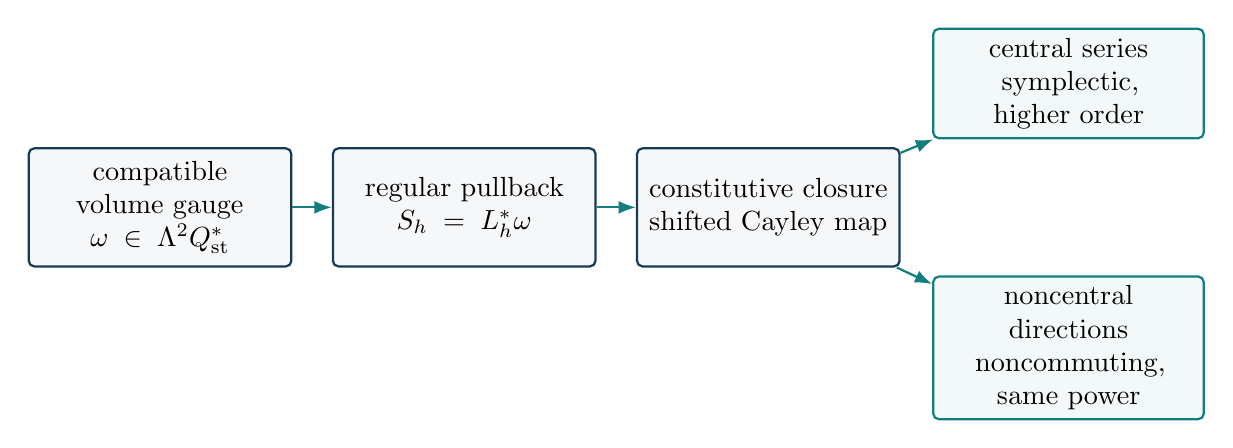
\begin{tikzpicture}[
  node distance=5mm,
  box/.style={draw=axblue,rounded corners=2pt,thick,align=center,
              minimum height=15mm,text width=31mm,fill=axblue!4},
  branch/.style={draw=axteal,rounded corners=2pt,thick,align=center,
                 minimum height=13mm,text width=32mm,fill=axteal!5},
  arr/.style={-{Latex[length=2.2mm]},thick,draw=axteal}
]
\node[box] (volume) {compatible volume gauge\\\(\omega\in\Lambda^2Q_{\rm st}^*\)};
\node[box,right=of volume] (cap) {regular pullback\\\(S_h=L_h^*\omega\)};
\node[box,right=of cap] (cayley) {constitutive closure\\shifted Cayley map};
\node[branch,above right=1mm and 4mm of cayley] (central)
 {central series\\symplectic, higher order};
\node[branch,below right=1mm and 4mm of cayley] (noncentral)
 {noncentral directions\\noncommuting, same power};
\draw[arr] (volume) -- (cap);
\draw[arr] (cap) -- (cayley);
\draw[arr] (cayley) -- (central);
\draw[arr] (cayley) -- (noncentral);
\end{tikzpicture}
\caption{Architecture of the construction.  Compatibility is classified
in the volume, transported to the caps, and closed through a Cayley chart.
Only after the constitutive generator \(A_N=\mathcal J_NQ_N\) is fixed
does the cap space split operationally into a central accuracy hierarchy
and noncentral design directions; both retain the same contracted power
identity.}
\label{fig:paper-architecture}
\end{figure}

\paragraph{Order convention.}
Every order statement below concerns matrix/operator convergence to
\(e^{hA_N}\) as \(h\to0\) for a \emph{fixed finite-dimensional linear
semidiscrete generator} \(A_N\), with constants allowed to depend on
\(N\).  It is neither a universal Runge--Kutta order statement for
nonlinear vector fields nor a simultaneous space--time convergence
theorem.  The nonlinear section establishes the chain rule and energy
identity, not the linear hierarchy's order.

\begin{definition}[Local matrix defect and global operator order]
\label{def:matrix-order}
For fixed \(A_N\), a one-step family \(M_h\) has \emph{local matrix defect
of order \(p+1\)} if
\begin{equation}\label{eq:local-matrix-order}
 \norm{M_h-e^{hA_N}}=O(h^{p+1})\qquad(h\to0)
\end{equation}
in any matrix norm.  It has \emph{global operator order \(p\)} on bounded
time intervals if, for each fixed \(T>0\) and \(n=T/h\in\mathbb N\),
\begin{equation}\label{eq:global-operator-order}
 \norm{M_h^n-e^{TA_N}}=O(h^p).
\end{equation}
For a consistent finite-dimensional family satisfying
\cref{eq:local-matrix-order}, the telescoping identity
\[
 M_h^n-e^{TA_N}
 =\sum_{k=0}^{n-1}M_h^{n-1-k}
  (M_h-e^{hA_N})e^{khA_N}
\]
gives \cref{eq:global-operator-order}.  Thus the one-power shift used
below is an explicit fixed-\(A_N\) matrix estimate.
\end{definition}

\paragraph{Terminology for ``exact.''}
The adjective is always qualified by its object.  \emph{Exact power} or
\emph{exact energy} means an algebraic identity at the discrete level;
\emph{exact elimination} means equality of two finite-dimensional Schur
reductions; \emph{exact order} means that the displayed leading error
coefficient is nonzero; and \emph{exact-flow gauge} refers specifically to
the Cayley coordinate of \(e^{hA_N}\).  None of these phrases asserts a
simultaneous continuum limit unless such a limit is stated separately.

\paragraph{Notation.}
All spaces are finite-dimensional and real. A vector space \(V\) and its
dual \(V^*\) are distinguished until coordinates are chosen. In
coordinates, covectors are represented by columns and paired by transpose.
For an invertible skew matrix \(J\), we write \(\Omega=J^{-1}\).
The state dimension is \(n\); in symplectic statements \(n=2m\).

\section{The affine Stokes-pairing principle}

We first isolate the algebra that is shared by spatial integration by parts
and the temporal discrete chain rule.

\begin{definition}[Discrete Stokes data]
Let \(E,F\) be vector spaces, let \(D:E\to F\) be linear, and let
\(b:E\times E\to\R\) be a symmetric bilinear boundary form. A bilinear
map \(M:E\times F\to\R\) is \emph{Stokes compatible} if
\begin{equation}\label{eq:stokes-compatibility}
 M(z,Dw)+M(w,Dz)=b(z,w)
 \qquad (z,w\in E).
\end{equation}
\end{definition}

\begin{theorem}[Active affine Stokes family]\label{thm:affine-stokes}
Let \(K=\ker D\), \(I=\operatorname{im}D\), and
\(r=\operatorname{rank}D\). A compatible pairing exists if and only if
\begin{equation}\label{eq:kernel-obstruction}
 b(k,\ell)=0\qquad(k,\ell\in K).
\end{equation}
On the active flow space \(I\), if \(M_0\) is one compatible pairing,
all compatible restrictions are
\begin{equation}\label{eq:abstract-gauge}
 M_\omega(z,Dw)=M_0(z,Dw)+\omega([z],[w]),
 \qquad \omega\in\Lambda^2(E/K)^*.
\end{equation}
Consequently the active solution set is an affine space of dimension
\begin{equation}\label{eq:active-dimension}
 \frac{r(r-1)}2.
\end{equation}
If pairings are required on all of \(E\times F\), their values transverse
to \(I\) are unconstrained.  If \(\mathcal H\) denotes the full
homogeneous direction, it fits into the short exact sequence
\begin{equation}\label{eq:full-affine-direction}
 0\longrightarrow \operatorname{Bil}(E,F/I;\R)
 \longrightarrow\mathcal H
 \longrightarrow\Lambda^2(E/K)^*
 \longrightarrow0.
\end{equation}
Every choice of a complement of \(I\) in \(F\) splits this sequence, but
the splitting is not canonical.  The full direction has dimension
\(r(r-1)/2+\dim(E)(\dim(F)-r)\).
\end{theorem}

\begin{proof}
Necessity follows from \cref{eq:stokes-compatibility} with \(z,w\in K\).
Assume \cref{eq:kernel-obstruction}. Choose a section
\(R:I\to E\) of \(D:E\to I\), and write \(z=k_z+RDz\). Define, for
\(g\in I\),
\[
 M_0(z,g)=\tfrac12 b(RDz,Rg)+b(k_z,Rg).
\]
Substitution and \cref{eq:kernel-obstruction} verify compatibility on
\(I\).  Choosing a complement of \(I\) in \(F\) and extending arbitrarily
produces a pairing on all of \(E\times F\).

If \(M\) and \(M_0\) are compatible, their difference \(N=M-M_0\) obeys
\[
 N(z,Dw)+N(w,Dz)=0.
\]
Taking \(w\in K\) gives \(N(w,Dz)=0\) for every \(z\), hence \(N\) factors
through \(E/K\) in its first argument.  The induced bijection
\(\bar D:E/K\to I\) identifies the two active arguments, so the induced
bilinear form is alternating. Conversely,
every alternating form in \cref{eq:abstract-gauge} cancels from the
symmetric identity.  This proves the active classification.  Finally,
compatibility evaluates the second argument only on \(I\).  Restriction to
\(I\) maps \(\mathcal H\) onto \(\Lambda^2(E/K)^*\), and its kernel
consists precisely of bilinear forms vanishing on \(I\), equivalently
forms on \(E\times(F/I)\).  This proves the exact sequence and the
dimension formula.
\end{proof}

\begin{remark}
The Stokes-visible active gauge is intrinsically an alternating two-form on
the quotient \(E/\ker D\), not a skew matrix until a basis and an
identification with its dual are selected.  The kernel term in
\cref{eq:full-affine-direction} is invisible to Stokes compatibility and
should not be counted as an active gauge.  This distinction becomes
essential for a space--time differential, whose image is constrained by
integrability.
\end{remark}

\begin{corollary}[Recovery of the polynomial spatial freedom]
\label{cor:2012-dimension}
For \(E=\cP_N\), \(F=\cP_{N-1}\), and
\(D=\dd/\dd z\), the derivative is onto, \(\dim F=N\), and the active
compatible family has dimension
\[
 \frac{N(N-1)}2.
\]
Thus the freedom in the polynomial Stokes construction of
\cite{moulla2012} is the spatial instance of
\cref{thm:affine-stokes}, rather than only an analogy based on Gaussian
orthogonality.
\end{corollary}

\section{Stokes' theorem on the space--time cylinder}

Let \(\Omega\) be an oriented \(d\)-dimensional manifold with boundary
and let
\[
 Z=[0,T]\times\Omega
\]
carry the product orientation.  Its oriented boundary is
\begin{equation}\label{eq:cylinder-boundary}
 \partial Z=
 (\{T\}\times\Omega)-(\{0\}\times\Omega)
 \;\cup\;([0,T]\times\partial\Omega).
\end{equation}
The first two components will be called the temporal caps and the last one
the lateral mantle.

\begin{proposition}[One identity on the cylinder]
\label{prop:continuous-cylinder}
For \(\alpha\in\Omega^k(Z)\) and
\(\beta\in\Omega^{d-k}(Z)\),
\begin{equation}\label{eq:continuous-stokes-cylinder}
 \int_Z \dd\alpha\wedge\beta
 +(-1)^k\int_Z\alpha\wedge\dd\beta
 =\int_{\partial Z}\operatorname{tr}\alpha\wedge
                   \operatorname{tr}\beta.
\end{equation}
The right-hand side splits according to
\cref{eq:cylinder-boundary} into a final-minus-initial cap term and a
lateral boundary term.
\end{proposition}

\begin{proof}
The graded Leibniz rule gives
\(
 \dd(\alpha\wedge\beta)
 =\dd\alpha\wedge\beta+(-1)^k\alpha\wedge\dd\beta
\).
Apply Stokes' theorem and use the product orientation of
\cref{eq:cylinder-boundary}.
\end{proof}

\begin{corollary}[Port-Hamiltonian balance as a cylinder law]
\label{cor:continuous-ph-cylinder}
Suppose that a distributed port-Hamiltonian system satisfies
\[
 \partial_t x=(\mathcal J-\mathcal R)e,
 \qquad e=\frac{\delta H}{\delta x},
 \qquad \mathcal R\succeq0,
\]
and that the Green identity for \(\mathcal J\) is
\[
 \ip{e}{\mathcal J e}_{\Omega}
 =\ip{y}{u}_{\partial\Omega}.
\]
Then
\begin{equation}\label{eq:continuous-power-cylinder}
 H(x(T))-H(x(0))
 =\int_0^T\ip{y}{u}_{\partial\Omega}\,\dd t
  -\int_0^T\ip{e}{\mathcal R e}_{\Omega}\,\dd t.
\end{equation}
Thus stored energy on the temporal caps and supplied power through the
lateral mantle are components of one oriented boundary balance.
\end{corollary}

\begin{proof}
The variational chain rule and the evolution equation give
\[
 \frac{\dd}{\dd t}H(x(t))
 =\ip{e}{(\mathcal J-\mathcal R)e}_{\Omega}
 =\ip{e}{\mathcal J e}_{\Omega}
  -\ip{e}{\mathcal R e}_{\Omega}.
\]
Use the Green identity and integrate in time.  This is the
port-Hamiltonian specialization of the cap--mantle split in
\cref{prop:continuous-cylinder}.
\end{proof}

\section{Discrete cylinders and the full space--time gauge}

\subsection{The temporal--spatial total complex}

\begin{definition}[Finite graded Stokes complex]
\label{def:graded-stokes}
A finite cochain complex \((C^\bullet,d)\) of formal dimension \(m\) is
equipped with a graded Stokes pairing if it has bilinear maps
\[
 I_k:C^k\times C^{m-k}\to\R
\]
and boundary maps \(B_k\) such that, for
\(a\in C^k\) and \(b\in C^{m-k-1}\),
\begin{equation}\label{eq:graded-discrete-stokes}
 I_{k+1}(da,b)+(-1)^kI_k(a,db)=B_k(a,b).
\end{equation}
The boundary maps include the appropriate discrete traces.  This is the
cochain form of integration by parts; no metric or constitutive operator
is included in the definition.
\end{definition}

Let \((C_t^\bullet,d_t)\) and \((C_x^\bullet,d_x)\) be finite cochain
complexes.  Their total complex is
\begin{equation}\label{eq:total-complex}
 C_{\rm st}^q=\bigoplus_{r+s=q}C_t^r\otimes C_x^s,
\end{equation}
with, on a homogeneous temporal cochain \(a\in C_t^r\),
\begin{equation}\label{eq:total-differential}
 d_{\rm st}(a\otimes b)
 =d_ta\otimes b+(-1)^r a\otimes d_xb.
\end{equation}
In matrices this is
\begin{equation}\label{eq:total-differential-matrix}
 D_{\rm st}=D_t\otimes I+\Gamma_t\otimes D_x,
\end{equation}
where \(\Gamma_t\) acts by \((-1)^r\) on temporal degree \(r\).

\begin{proposition}[Complex property and signed product Stokes formula]
\label{prop:total-complex}
The total differential satisfies \(d_{\rm st}^2=0\).
Assume that the factor complexes have formal dimensions \(m_t,m_x\) and
carry the pairings of \cref{def:graded-stokes}.  For homogeneous simple
tensors of complementary bidegrees, define
\begin{equation}\label{eq:signed-tensor-pairing}
 I_{\rm st}(a_t\otimes a_x,c_t\otimes c_x)
 =(-1)^{|a_x||c_t|}
 I_t(a_t,c_t)I_x(a_x,c_x).
\end{equation}
Let \(|a_t|=r\), \(|a_x|=s\).  A homogeneous element of total degree
\(m_t+m_x-r-s-1\) has the two complementary components
\[
 b^{(t)}=c_t\otimes c_x,\qquad
 (|c_t|,|c_x|)=(m_t-r-1,m_x-s),
\]
and
\[
 b^{(x)}=e_t\otimes e_x,\qquad
 (|e_t|,|e_x|)=(m_t-r,m_x-s-1).
\]
Then the total boundary form is
\begin{align}
 B_{\rm st}(a,b)
 &=(-1)^{s(m_t-r-1)}
   B_t(a_t,c_t)I_x(a_x,c_x)\notag\\
 &\quad+(-1)^{m_t+s(m_t-r)}
   I_t(a_t,e_t)B_x(a_x,e_x).
 \label{eq:signed-product-boundary}
\end{align}
The first term is the temporal-cap contribution and the second is the
spatial-mantle contribution, including the product-orientation sign.
\end{proposition}

\begin{proof}
For a homogeneous simple tensor,
\begin{align*}
 d_{\rm st}^2(a\otimes b)
 &=d_t^2a\otimes b
   +(-1)^{r+1}d_ta\otimes d_xb
   +(-1)^r d_ta\otimes d_xb
   +a\otimes d_x^2b=0.
\end{align*}
For \(b^{(t)}\), only the two temporal derivatives can pair factorwise.
Using \cref{eq:signed-tensor-pairing}, their sum is
\[
 (-1)^{s(m_t-r-1)}
 \bigl[I_t(d_ta_t,c_t)+(-1)^rI_t(a_t,d_tc_t)\bigr]
 I_x(a_x,c_x),
\]
which is the first term of \cref{eq:signed-product-boundary}.  For
\(b^{(x)}\), the sign \((-1)^r\) in the spatial part of
\cref{eq:total-differential} combines with the interchange sign in
\cref{eq:signed-tensor-pairing}.  The result is
\[
 (-1)^{m_t+s(m_t-r)}I_t(a_t,e_t)
 \bigl[I_x(d_xa_x,e_x)+(-1)^sI_x(a_x,d_xe_x)\bigr],
\]
which gives the mantle term.  Linearity handles sums of bidegrees.  This
also displays explicitly why the two boundary pieces add while the mixed
interior derivatives cancel.
\end{proof}

The affine freedom of the genuine total complex can now be stated without
replacing it by a directional gradient.  Let \(m\) be its formal dimension
and fix \(q\in\{0,\ldots,m-1\}\).  Set
\begin{equation}\label{eq:graded-double-spaces}
 \mathbb E_q=C_{\rm st}^q\oplus C_{\rm st}^{m-q-1},\qquad
 \mathbb F_q=C_{\rm st}^{q+1}\oplus C_{\rm st}^{m-q},
\end{equation}
and define
\begin{equation}\label{eq:graded-double-differential}
 \mathbb D_q(a,b)=(d_{\rm st}a,d_{\rm st}b).
\end{equation}
For \(z=(a,b)\) and \(\widehat z=(\widehat a,\widehat b)\), introduce the
symmetric doubled boundary form
\begin{equation}\label{eq:graded-double-boundary}
 \mathbf b_q(z,\widehat z)
 =B_q(a,\widehat b)+B_q(\widehat a,b).
\end{equation}

\begin{theorem}[Affine classification for the genuine total complex]
\label{thm:graded-affine}
Put
\[
 U_q=C_{\rm st}^q/\ker d_{\rm st}^q,
 \qquad
 V_q=C_{\rm st}^{m-q-1}/\ker d_{\rm st}^{m-q-1}.
\]
The pairing
\begin{equation}\label{eq:graded-double-pairing}
 \mathbb M_q\bigl((a,b),(f,g)\bigr)
 =I_{q+1}(f,b)+(-1)^qI_q(a,g)
\end{equation}
is compatible with \(\mathbb D_q\) and \(\mathbf b_q\).  Without a degree
restriction, the active compatible family is affine over
\begin{equation}\label{eq:graded-unrestricted-gauge}
 \Lambda^2(U_q\oplus V_q)^*.
\end{equation}
If the pairing is required to preserve complementary degree---so that it
pairs \(C_{\rm st}^q\) only with \(dC_{\rm st}^{m-q-1}\), and
\(C_{\rm st}^{m-q-1}\) only with \(dC_{\rm st}^{q}\)---its homogeneous
freedom is instead exactly
\begin{equation}\label{eq:graded-active-gauge}
 \boxed{\quad \operatorname{Bil}(U_q,V_q;\mathbb R)
       \simeq U_q^*\otimes V_q^*.\quad}
\end{equation}
Thus cancellations between different bidegrees are incorporated through
the actual kernels of the total differential.
\end{theorem}

\begin{proof}
For \(z=(a,b)\) and \(\widehat z=(\widehat a,\widehat b)\), the left-hand
side of the symmetric compatibility identity is
\begin{align*}
 &\mathbb M_q(z,\mathbb D_q\widehat z)
  +\mathbb M_q(\widehat z,\mathbb D_qz)\\
 &=I_{q+1}(d\widehat a,b)+(-1)^qI_q(\widehat a,db)
  +I_{q+1}(da,\widehat b)+(-1)^qI_q(a,d\widehat b)\\
 &=B_q(\widehat a,b)+B_q(a,\widehat b),
\end{align*}
which is \cref{eq:graded-double-boundary}.  Since
\(\ker\mathbb D_q=\ker d_{\rm st}^q\oplus
\ker d_{\rm st}^{m-q-1}\), \cref{thm:affine-stokes} gives
\cref{eq:graded-unrestricted-gauge}.

For the degree-preserving subfamily, let a homogeneous correction have
off-diagonal components \(N_1(a,d\widehat b)\) and
\(N_2(b,d\widehat a)\).  After quotienting the two kernels, compatibility
with zero boundary requires
\[
 N_1(u,\widehat v)+N_2(v,\widehat u)
 +N_1(\widehat u,v)+N_2(\widehat v,u)=0.
\]
Taking \(\widehat u=0\) and \(v=0\) gives
\(N_2(\widehat v,u)=-N_1(u,\widehat v)\).  Hence one arbitrary bilinear
form \(\eta\in\operatorname{Bil}(U_q,V_q;\mathbb R)\) determines both
components through
\begin{equation}\label{eq:graded-homogeneous-correction}
 N_\eta\bigl((a,b),\mathbb D_q(\widehat a,\widehat b)\bigr)
 =\eta([a],[\widehat b])-\eta([\widehat a],[b]),
\end{equation}
and every degree-preserving correction is obtained in this way.
\end{proof}

\begin{remark}[The total and stacked kernels are different]
\label{rem:total-versus-stacked}
Take two copies of the complex
\(0\to\mathbb R\xrightarrow{1}\mathbb R\to0\).  At total degree one,
the total differential is, up to orientation,
\(d_{\rm st}(a,b)=b-a\); its kernel is the diagonal even though both
factor differentials have zero kernel.  Therefore the formula
\(\ker D_{\rm st}=K_t\otimes K_x\) below is not a formula for an arbitrary
total-complex differential.  It belongs to the stacked one-bidegree map,
where the two directional derivatives are retained as separate output
components.
\end{remark}

The preceding theorem treats the genuine graded total complex.  The
finite tensor cells used later employ a related but distinct stacked map.
Let
\((E_a,F_a,D_a,b_a,M_a)\), \(a\in\{t,x\}\), be compatible Stokes data,
and let \(G_a:E_a\times E_a\to\R\) be symmetric interior pairings.  Put
\begin{align}
 E_{\rm st}&=E_t\otimes E_x,\label{eq:Est}\\
 F_{\rm st}&=(F_t\otimes E_x)\oplus(E_t\otimes F_x),\label{eq:Fst}\\
 D_{\rm st}z&=((D_t\otimes I)z,(I\otimes D_x)z),\label{eq:Dst-gradient}
\end{align}
where the sign \(\Gamma_t\) is inserted in the second component when the
chosen bidegree requires it.  Unlike \cref{eq:total-differential}, the two
directional images in \cref{eq:Dst-gradient} are not added.

\begin{theorem}[Product representative and cylinder boundary]
\label{thm:product-representative}
There is a compatible product representative \(M_{\rm st}^0\) defined on
simple tensors by
\begin{align}
 &M_{\rm st}^0
 \bigl(z_t\otimes z_x,
       (f_t\otimes e_x,e_t\otimes f_x)\bigr)\notag\\
 &\qquad=
 M_t(z_t,f_t)G_x(z_x,e_x)
 +G_t(z_t,e_t)M_x(z_x,f_x),
 \label{eq:product-representative}
\end{align}
and extended bilinearly.  Its boundary form is
\begin{equation}\label{eq:product-boundary}
 b_{\rm st}=b_t\otimes G_x+G_t\otimes b_x.
\end{equation}
The first summand is supported on the temporal caps and the second on the
spatial mantle.
\end{theorem}

\begin{proof}
It suffices to test pure tensors \(z=z_t\otimes z_x\) and
\(w=w_t\otimes w_x\).  Substitution of \cref{eq:Dst-gradient} into
\cref{eq:product-representative} gives
\begin{align*}
 &\bigl[M_t(z_t,D_tw_t)+M_t(w_t,D_tz_t)\bigr]
   G_x(z_x,w_x)\\
 &\quad+G_t(z_t,w_t)
   \bigl[M_x(z_x,D_xw_x)+M_x(w_x,D_xz_x)\bigr].
\end{align*}
Factor compatibility turns this expression into
\(b_t(z_t,w_t)G_x(z_x,w_x)+G_t(z_t,w_t)b_x(z_x,w_x)\).
Pure tensors span \(E_{\rm st}\), proving the result.  In the graded
version the Koszul sign in \cref{eq:total-differential} produces the
oriented sign in the mantle term.
\end{proof}

\subsection{Classification and sector decomposition}

Write \(K_a=\ker D_a\), \(n_a=\dim E_a\), and
\(k_a=\dim K_a\) for \(a\in\{t,x\}\).

\begin{theorem}[Full active gauge of the stacked cylinder cell]
\label{thm:space-time-gauge}
For \cref{eq:Dst-gradient},
\begin{equation}\label{eq:space-time-kernel}
 K_{\rm st}:=\ker D_{\rm st}=K_t\otimes K_x.
\end{equation}
Consequently
\begin{equation}\label{eq:space-time-rank}
 r_{\rm st}:=\operatorname{rank}D_{\rm st}
 =n_tn_x-k_tk_x.
\end{equation}
Every active compatible space--time pairing is
\begin{equation}\label{eq:space-time-affine-family}
 M_{\rm st}^{\omega}(z,D_{\rm st}w)
 =M_{\rm st}^0(z,D_{\rm st}w)+\omega([z],[w]),
 \qquad
 \omega\in\mathcal G_{\rm st},
\end{equation}
where
\begin{equation}\label{eq:intrinsic-space-time-gauge}
 \boxed{\quad
 \mathcal G_{\rm st}
 =\Lambda^2(E_{\rm st}/K_{\rm st})^*.
 \quad}
\end{equation}
Its dimension is
\begin{equation}\label{eq:space-time-gauge-dimension}
 \dim\mathcal G_{\rm st}
 =\frac{r_{\rm st}(r_{\rm st}-1)}2.
\end{equation}
\end{theorem}

\begin{proof}
The kernel of \(D_t\otimes I\) is \(K_t\otimes E_x\), while the kernel
of \(I\otimes D_x\) is \(E_t\otimes K_x\).  Their intersection is
\(K_t\otimes K_x\), proving \cref{eq:space-time-kernel}; rank--nullity
gives \cref{eq:space-time-rank}.  The product representative in
\cref{thm:product-representative} proves existence, and
\cref{thm:affine-stokes} applied to \(D_{\rm st}\) gives
\cref{eq:space-time-affine-family}--\cref{eq:space-time-gauge-dimension}.
\end{proof}

\begin{proposition}[Canonical pure--mixed filtration]
\label{prop:canonical-sector-sequence}
Let
\[
 Q_{\rm st}=(E_t\otimes E_x)/(K_t\otimes K_x),\qquad
 \overline E_t=E_t/K_t,\quad \overline E_x=E_x/K_x.
\]
There is a canonical short exact sequence
\begin{equation}\label{eq:canonical-sector-sequence}
 0\longrightarrow
 (\overline E_t\otimes K_x)\oplus(K_t\otimes\overline E_x)
 \xrightarrow{\;\jmath\;}Q_{\rm st}
 \xrightarrow{\;\pi_{tx}\;}
 \overline E_t\otimes\overline E_x
 \longrightarrow0.
\end{equation}
The subspace on the left contains the pure temporal and pure spatial
directions.  The quotient on the right is the canonical mixed sector.
A choice of complements of \(K_t\) and \(K_x\) supplies a natural
factorized splitting of this filtration.  General linear sections of
\(\pi_{tx}\) need not arise from such a pair of complements.
\end{proposition}

\begin{proof}
The tensor product of the quotient maps
\(E_t\to\overline E_t\) and \(E_x\to\overline E_x\) vanishes on
\(K_t\otimes K_x\), hence induces \(\pi_{tx}\).  Its kernel is the image
of \(E_t\otimes K_x+K_t\otimes E_x\) modulo
\(K_t\otimes K_x\).  Quotienting the intersection
\((E_t\otimes K_x)\cap(K_t\otimes E_x)=K_t\otimes K_x\)
identifies this kernel with the direct sum on the left of
\cref{eq:canonical-sector-sequence}.  Surjectivity follows from that of
the two factor quotient maps.
\end{proof}

\begin{corollary}[Temporal, spatial, and mixed sectors]
\label{cor:gauge-sectors}
Choose complements \(E_t=K_t\oplus U_t\) and
\(E_x=K_x\oplus U_x\).  Then
\begin{equation}\label{eq:quotient-sector-split}
 E_{\rm st}/K_{\rm st}
 \simeq Q_t\oplus Q_x\oplus Q_{tx},
\end{equation}
where
\[
 Q_t=U_t\otimes K_x,
 \qquad Q_x=K_t\otimes U_x,
 \qquad Q_{tx}=U_t\otimes U_x
 \simeq\overline E_t\otimes\overline E_x.
\]
Accordingly,
\begin{equation}\label{eq:wedge-sector-split}
 \mathcal G_{\rm st}
 \simeq
 \bigoplus_{a\in\{t,x,tx\}}\Lambda^2Q_a^*
 \;\oplus\!
 \bigoplus_{a<b}Q_a^*\otimes Q_b^*.
\end{equation}
The summands contain pure temporal, pure spatial, mixed, and cross-sector
gauges.  The total space \(\mathcal G_{\rm st}\), the pure subspace, and
the mixed quotient in \cref{eq:canonical-sector-sequence} are intrinsic;
only the displayed direct-sum splitting depends on the chosen complements.
\end{corollary}

\begin{proof}
Expanding
\((K_t\oplus U_t)\otimes(K_x\oplus U_x)\) and quotienting by
\(K_t\otimes K_x\) gives \cref{eq:quotient-sector-split}.  For a direct
sum \(Q=Q_1\oplus Q_2\oplus Q_3\), the standard exterior-square identity
is
\(
 \Lambda^2Q^*=\bigoplus_i\Lambda^2Q_i^*
 \oplus\bigoplus_{i<j}Q_i^*\otimes Q_j^*
\), which proves \cref{eq:wedge-sector-split}.
\end{proof}

\begin{proposition}[Pure-axis embeddings and boundary reduction]
\label{prop:boundary-reductions}
For nonzero \(k_t\in K_t\) and \(k_x\in K_x\), the maps
\begin{align*}
 \iota_t:E_t/K_t&\longrightarrow E_{\rm st}/K_{\rm st},
 &[z_t]&\longmapsto[z_t\otimes k_x],\\
 \iota_x:E_x/K_x&\longrightarrow E_{\rm st}/K_{\rm st},
 &[z_x]&\longmapsto[k_t\otimes z_x]
\end{align*}
are injective.  Pullback by \(\iota_t\) and \(\iota_x\) sends a
space--time gauge to its pure temporal and pure spatial restrictions.  In
particular, the time-constant pullback contains the polynomial spatial
gauges of \cite{moulla2012}.  A cap-to-cap temporal method on the full
spatial state space is obtained only after eliminating the interior
spatial flows; it generally receives contributions from
\(Q_t\oplus Q_{tx}\).  The next sections classify that reduced boundary
gauge.  A gauge supported entirely on \(Q_{tx}\) can be nonzero while both
pure-axis restrictions vanish.
\end{proposition}

\begin{proof}
If \(z_t\otimes k_x\in K_t\otimes K_x\) and \(k_x\ne0\), then
\(z_t\in K_t\); hence \(\iota_t\) is injective.  The spatial statement is
identical.  Alternating forms pull back functorially.  Finally a form
supported on \(Q_{tx}\) vanishes on the images of both pure embeddings.
\end{proof}

\subsection{Regular volume-to-cap reduction}

The pullbacks in \cref{prop:boundary-reductions} restrict a gauge along
pure axes.  A numerical time step requires a different operation: the
interior equations must first be solved and the resulting active volume
field restricted to its cap data.  This operation depends on the Dirac
relation, the constitutive closure, the boundary causality, and the step
size; it is not determined by the Stokes pairing alone.

Let
\[
 Q_{\rm st}=E_{\rm st}/K_{\rm st}
\]
be the active volume space and let \(Q_\partial\) be the chosen active cap
space.  After fixing the four ingredients above, call the reduction
\emph{regular} if the interior equations determine a linear reconstruction
\begin{equation}\label{eq:regular-lifting}
 L_h:Q_\partial\longrightarrow Q_{\rm st}.
\end{equation}
The notation permits \(L_h\) to depend on the selected constitutive law
and on \(h\), but it is held fixed while the following affine gauge
reduction is classified.

\begin{theorem}[Exact visibility sequence for volume-to-cap gauges]
\label{thm:volume-cap-reduction}
For a regular reconstruction \(L_h\), the homogeneous volume-to-cap reduction is
the pullback map
\begin{equation}\label{eq:volume-cap-pullback}
 \mathcal R_{L_h}:\Lambda^2Q_{\rm st}^*
 \longrightarrow\Lambda^2Q_\partial^*,
 \qquad
 \mathcal R_{L_h}(\omega)=L_h^*\omega,
\end{equation}
where
\[
 (L_h^*\omega)(\xi,\zeta)
 =\omega(L_h\xi,L_h\zeta).
\]
Put
\[
 W_h=\operatorname{im}L_h,\qquad
 K_{\partial,h}=\ker L_h,\qquad r_h=\operatorname{rank}L_h.
\]
Then
\begin{equation}\label{eq:volume-cap-image}
 \operatorname{im}\mathcal R_{L_h}
 =
 \left\{\eta\in\Lambda^2Q_\partial^*:
 \iota_k\eta=0\ \text{for every }k\in K_{\partial,h}\right\}
 \simeq\Lambda^2(Q_\partial/K_{\partial,h})^*,
\end{equation}
and
\begin{equation}\label{eq:volume-cap-kernel}
 \ker\mathcal R_{L_h}
 =
 \left\{\omega\in\Lambda^2Q_{\rm st}^*:
 \omega|_{W_h\times W_h}=0\right\}.
\end{equation}
Equivalently, restriction to \(W_h\) gives the short exact sequence
\begin{equation}\label{eq:volume-cap-exact-sequence}
 0\longrightarrow\ker\mathcal R_{L_h}
 \longrightarrow\Lambda^2Q_{\rm st}^*
 \xrightarrow{\;\mathcal R_{L_h}\;}
 \Lambda^2(Q_\partial/K_{\partial,h})^*
 \longrightarrow0.
\end{equation}
Consequently,
\begin{align}
 \dim\operatorname{im}\mathcal R_{L_h}
 &=\frac{r_h(r_h-1)}2,\label{eq:volume-cap-image-dimension}\\
 \dim\ker\mathcal R_{L_h}
 &=\binom{\dim Q_{\rm st}}2-\binom{r_h}2.
 \label{eq:volume-cap-kernel-dimension}
\end{align}
If \(L_h\) is injective, every cap gauge has a volume extension.  If
\(L_h\) is surjective, no nonzero volume gauge is invisible on all cap
data.  In particular, an isomorphism \(L_h\) induces an isomorphism of
gauge spaces.
\end{theorem}

\begin{proof}
If \(k\in K_{\partial,h}\), then
\((L_h^*\omega)(k,\xi)=\omega(0,L_h\xi)=0\), proving the inclusion from
left to right in \cref{eq:volume-cap-image}.  Conversely, every
\(\eta\) satisfying the annihilation condition descends uniquely to an
alternating form on \(Q_\partial/K_{\partial,h}\).  The induced map
\[
 \overline L_h:Q_\partial/K_{\partial,h}\longrightarrow W_h
\]
is an isomorphism.  Transport \(\eta\) to \(W_h\) by this isomorphism and
extend the resulting alternating form from \(W_h\) to \(Q_{\rm st}\)
using any linear complement of \(W_h\).  Its pullback is \(\eta\), so
\cref{eq:volume-cap-image} and surjectivity in
\cref{eq:volume-cap-exact-sequence} follow.

The pullback vanishes exactly when \(\omega\) vanishes on every pair of
vectors in \(W_h\), which is \cref{eq:volume-cap-kernel}.  Since
\(\dim W_h=r_h\), the two dimension formulas follow.  Injectivity of
\(L_h\) means \(K_{\partial,h}=0\), while surjectivity means
\(W_h=Q_{\rm st}\); the final claims are immediate.
\end{proof}

\begin{corollary}[Affine reduction and gauge-invariant power]
\label{cor:affine-volume-cap}
Assume that a reference compatible volume pairing reduces, under the same
fixed reconstruction, to a cap pairing \(m_{\partial,0}\).  Then the full reduced
family is
\begin{equation}\label{eq:reduced-affine-family}
 m_{\partial,\omega}
 =m_{\partial,0}+L_h^*\omega.
\end{equation}
For every cap increment \(\xi\),
\[
 (L_h^*\omega)(\xi,\xi)=0.
\]
Thus the visible gauge changes the cap method but not its contracted power
identity.
\end{corollary}

\begin{corollary}[Intrinsic reduction of the mixed quotient]
\label{cor:mixed-visibility}
Let
\(Q_{tx}=\overline E_t\otimes\overline E_x\) and let
\(\pi_{tx}:Q_{\rm st}\to Q_{tx}\) be the canonical quotient map in
\cref{eq:canonical-sector-sequence}.  Pullback embeds the canonical mixed
gauges as \(\pi_{tx}^*\Lambda^2Q_{tx}^*\subset\Lambda^2Q_{\rm st}^*\), and
\begin{equation}\label{eq:intrinsic-mixed-pullback}
 \boxed{\quad
 \mathcal R_{L_h}\circ\pi_{tx}^*
 =(\pi_{tx}L_h)^*.
 \quad}
\end{equation}
If \(r_{tx,h}=\operatorname{rank}(\pi_{tx}L_h)\), then the visible
canonical mixed family has dimension
\begin{equation}\label{eq:mixed-visibility-dimension}
 \dim\operatorname{im}(\mathcal R_{L_h}\circ\pi_{tx}^*)
 =\binom{r_{tx,h}}2.
\end{equation}
Its kernel consists exactly of the forms on \(Q_{tx}\) that vanish on
\(\operatorname{im}(\pi_{tx}L_h)\times
\operatorname{im}(\pi_{tx}L_h)\), and has dimension
\[
 \binom{\dim Q_{tx}}2-\binom{r_{tx,h}}2.
\]
In particular, there exists a nonzero canonical mixed gauge whose cap
pullback is nonzero if and only if
\begin{equation}\label{eq:mixed-visibility-rank}
 \operatorname{rank}(\pi_{tx}L_h)\ge2.
\end{equation}
A prescribed nonzero mixed form may nevertheless belong to the kernel.
\end{corollary}

\begin{proof}
Functoriality gives
\(L_h^*\pi_{tx}^*=(\pi_{tx}L_h)^*\).  Apply
\cref{thm:volume-cap-reduction} to the single map \(\pi_{tx}L_h\).  The
image, kernel, and dimension statements follow verbatim and require no
choice of tensor complements.
\end{proof}

\begin{proposition}[Schur realization of the reconstruction]
\label{prop:schur-lifting}
Suppose a linear Dirac--constitutive cell has been partitioned into
interior variables \(z_i\) and cap variables \(\xi\), and its interior
equations are
\begin{equation}\label{eq:interior-block-system}
 K_{ii}(h)z_i+K_{i\partial}(h)\xi=0.
\end{equation}
If \(K_{ii}(h)\) is invertible, the regular reconstruction is
\begin{equation}\label{eq:schur-lifting}
 L_h\xi=
 \begin{bmatrix}
  -K_{ii}(h)^{-1}K_{i\partial}(h)\xi\\[1mm]\xi
 \end{bmatrix}.
\end{equation}
In coordinates, a volume gauge matrix \(\Omega_{\rm st}^\top
=-\Omega_{\rm st}\) reduces to
\begin{equation}\label{eq:schur-gauge}
 \Omega_\partial=L_h^\top\Omega_{\rm st}L_h.
\end{equation}
\end{proposition}

\begin{proof}
Equation \cref{eq:schur-lifting} is the unique solution of
\cref{eq:interior-block-system}; \cref{eq:schur-gauge} is the coordinate
form of \cref{eq:volume-cap-pullback}.
\end{proof}

\begin{theorem}[Trace-generated cell and exact raw realization]
\label{thm:trace-generated-condensation}
Let \(X\) be the active cap state space and \(Z_h\) a raw cell space.  Let
\(T_h:Z_h\to X\) be onto, let \(Q:X\to X^*\) be symmetric, and let
\(J:X^*\to X\) be skew.  For an alternating cap map
\(S_h:X\to X^*\), put
\begin{equation}\label{eq:trace-generated-volume-form}
 \Omega_h=T_h^*S_hT_h:Z_h\longrightarrow Z_h^*.
\end{equation}
It descends to \(\overline\Omega_h\) on
\(\overline Z_h=Z_h/\ker T_h\).  Given \(x_0\), consider the weak cell
equations for \(([z],e,x_1)\in\overline Z_h\times X^*\times X\):
\begin{align}
 \overline T_h[z]&=x_1-x_0,\label{eq:raw-cell-trace}\\
 x_1-x_0&=hJe,\label{eq:raw-cell-dirac}\\
 \overline T_h^*\bigl(e-Q\overline x\bigr)
 +\overline\Omega_h[z]&=0,
 \qquad \overline x=\tfrac12(x_0+x_1).
 \label{eq:raw-cell-constitutive}
\end{align}
Then the cap closure encoded by \(\Omega_h\) is recovered exactly by
elimination:
\begin{equation}\label{eq:condensed-cap-closure}
 e=Q\overline x-S_h(x_1-x_0)
\end{equation}
and its exact Schur complement is
\begin{equation}\label{eq:trace-generated-cap-map}
 \boxed{\quad
 \bigl(I+hJS_h-\tfrac h2JQ\bigr)x_1
 =\bigl(I+hJS_h+\tfrac h2JQ\bigr)x_0.
 \quad}
\end{equation}
Equation \cref{eq:trace-generated-cap-map} is always a linear relation.
If
\begin{equation}\label{eq:trace-generated-invertibility}
 I+hJS_h-\tfrac h2JQ
 \quad\text{is invertible},
\end{equation}
it defines a unique map from \(x_0\) to \(x_1\).  The physical variables
\((e,x_1)\) are independent of the representative
of \([z]\) and of the right inverse used to coordinatize the quotient.

In Euclidean coordinates, let the columns of \(N_h\) form an orthonormal
basis of \(\ker T_h\).  A square raw assembly, with a multiplier fixing
the null component, is
\begin{equation}\label{eq:raw-cell-block-system}
 \begin{bmatrix}
 T_h&0&-I&0\\
 0&-hJ&I&0\\
 \Omega_h&T_h^*&-\tfrac12T_h^*Q&N_h\\
 N_h^*&0&0&0
 \end{bmatrix}
 \begin{bmatrix}z\\e\\x_1\\\lambda\end{bmatrix}
 =
 \begin{bmatrix}-I\\I\\\tfrac12T_h^*Q\\0\end{bmatrix}x_0.
\end{equation}
Under \cref{eq:trace-generated-invertibility}, this square system is
invertible and its Schur map from \(x_0\) to \(x_1\) is exactly
\cref{eq:trace-generated-cap-map}.  Thus the prescribed cap gauge is not
attached as an additional reduced equation: it is encoded by the
trace-generated volume form and recovered exactly from the raw cell.
\end{theorem}

\begin{proof}
Because \(T_h\) is onto, the induced map
\(\overline T_h:\overline Z_h\to X\) is an isomorphism and
\(\overline T_h^*\) is injective.  Using
\cref{eq:trace-generated-volume-form,eq:raw-cell-trace}, the third cell
equation becomes
\[
 \overline T_h^*
 \bigl(e-Q\overline x+S_h(x_1-x_0)\bigr)=0.
\]
Injectivity gives \cref{eq:condensed-cap-closure}.  Substitution into
\cref{eq:raw-cell-dirac} gives
\[
 x_1-x_0=hJ\bigl(Q\overline x-S_h(x_1-x_0)\bigr),
\]
which rearranges to \cref{eq:trace-generated-cap-map}.  If
\(R_h:X\to Z_h\) is any right inverse, then
\[
 R_h^*\Omega_hR_h
 =(T_hR_h)^*S_h(T_hR_h)=S_h.
\]
Two right inverses differ by a map into \(\ker T_h\), on which
\(\Omega_h\) vanishes.  Finally, the last row of
\cref{eq:raw-cell-block-system} selects the orthogonal representative;
the third row is the unquotiented weak equation.  Eliminating
\((z,e,\lambda)\) reproduces the preceding calculation.  Under
\cref{eq:trace-generated-invertibility}, a homogeneous right-hand side
first gives \(x_1=e=0\) from the condensed equations, then \(z=0\) from
\(T_hz=0\) and \(N_h^*z=0\), and finally \(\lambda=0\).  The square raw
system is therefore invertible.
\end{proof}

\begin{figure}[t]
\centering
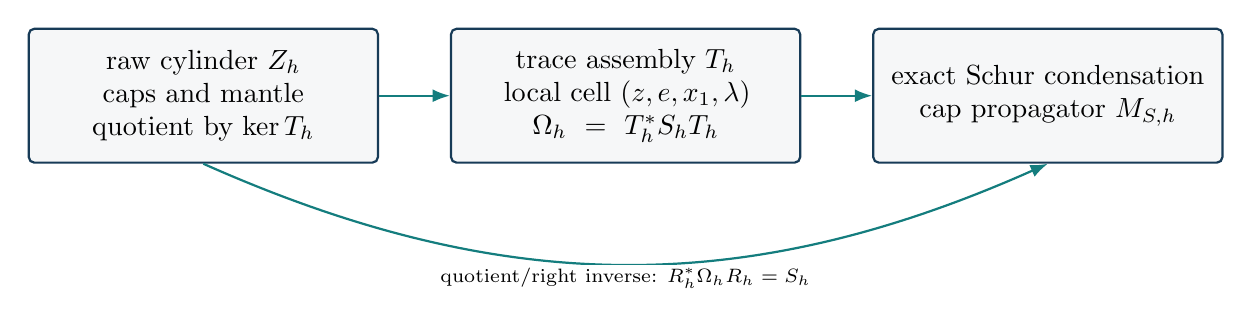
\begin{tikzpicture}[
  node distance=9mm,
  box/.style={draw=axblue,rounded corners=2pt,thick,align=center,
              minimum height=17mm,text width=42mm,fill=axblue!4},
  arr/.style={-{Latex[length=2.2mm]},thick,draw=axteal},
  lab/.style={font=\scriptsize,align=center,fill=white,inner sep=1pt}
]
\node[box] (raw) {raw cylinder \(Z_h\)\\caps and mantle\\quotient by \(\ker T_h\)};
\node[box,right=of raw] (cell) {trace assembly \(T_h\)\\local cell \((z,e,x_1,\lambda)\)\\\(\Omega_h=T_h^*S_hT_h\)};
\node[box,right=of cell] (cap) {exact Schur condensation\\cap propagator \(M_{S,h}\)};
\draw[arr] (raw) -- (cell);
\draw[arr] (cell) -- (cap);
\draw[arr] (raw.south) to[bend right=24]
 node[lab,below]{quotient/right inverse: \(R_h^*\Omega_hR_h=S_h\)} (cap.south);
\end{tikzpicture}
\caption{Exact raw-cell realization of a prescribed cap gauge.  The lower
identity is independent of the chosen section; the upper path shows that
the gauge encoded in \(\Omega_h=T_h^*S_hT_h\) is recovered exactly by
elimination.  No claim of selecting \(S_h\) from independent interior
dynamics is made here.}
\label{fig:dynamic-condensation}
\end{figure}

\begin{remark}[Singular interior problems]
If \(K_{ii}(h)\) is singular, the interior solution may be nonunique or
subject to compatibility constraints.  The reduction is then a linear
relation rather than a map \(L_h\), and composition of Dirac relations or
presymplectic reduction is required.  Likewise, if changing the volume
gauge changes the interior solve, one obtains \(L_h^\omega\) and the
global map \(\omega\mapsto(L_h^\omega)^*\omega\) need not be affine.
\Cref{thm:volume-cap-reduction} classifies the exact gauge freedom within
each fixed regular reduction chart; it does not hide these hypotheses.
\end{remark}

\begin{proposition}[Tangent reduction when the reconstruction depends on the gauge]
\label{prop:gauge-dependent-tangent}
Suppose \(\omega\mapsto L_h^\omega\) is differentiable and define
\[
 \mathcal F_h(\omega)=(L_h^\omega)^*\omega.
\]
For \(\xi,\zeta\in Q_\partial\),
\begin{align}
 D\mathcal F_h(\omega)[\delta\omega](\xi,\zeta)
 &=\delta\omega(L_h^\omega\xi,L_h^\omega\zeta)\notag\\
 &\quad+\omega(DL_h^\omega[\delta\omega]\xi,L_h^\omega\zeta)\notag\\
 &\quad+\omega(L_h^\omega\xi,DL_h^\omega[\delta\omega]\zeta).
 \label{eq:gauge-dependent-differential}
\end{align}
At the zero gauge,
\begin{equation}\label{eq:tangent-pullback}
 D\mathcal F_h(0)[\delta\omega]=L_h^{0*}\delta\omega.
\end{equation}
Thus the fixed-reconstruction pullback theorem is also the exact tangent
model of a gauge-dependent nonlinear reduction.  For the trace-generated
family in \cref{thm:trace-generated-condensation}, the stronger finite
identity holds because the quotient trace itself is gauge independent.
\end{proposition}

\begin{proof}
Differentiate
\(\omega(L_h^\omega\xi,L_h^\omega\zeta)\) by the product rule.  At
\(\omega=0\), the two terms containing the undifferentiated form vanish.
\end{proof}

\section{The complete two-point temporal gauge}

We now pass to the cap-to-cap problem obtained after eliminating interior
spatial flows, while keeping the spatial state space arbitrary.  In the
language of \cref{thm:volume-cap-reduction}, its gauge belongs to the image
of \(\mathcal R_{L_h}\) and can therefore contain the trace of mixed
space--time sectors precisely under \cref{eq:mixed-visibility-rank}.  This
is also the smallest setting in which the distinction between
gauge-invariant power and gauge-dependent symplecticity is visible.

\subsection{Temporal Stokes data}

Let \(V=\R^n\), let \(Q=Q^\top\), and define
\[
 H(x)=\tfrac12x^\top Qx,\qquad
 z=(x_0,x_1)\in E_t=V\oplus V,\qquad
 D_tz=x_1-x_0=:\Delta x.
\]
The polarized temporal boundary form is
\begin{equation}\label{eq:temporal-boundary}
 b_Q(z,w)=x_1^\top Qy_1-x_0^\top Qy_0,
 \qquad w=(y_0,y_1).
\end{equation}
Its restriction to \(K_t=\ker D_t=\{(x,x):x\in V\}\) vanishes. Hence
\cref{thm:affine-stokes} applies.

A linear two-point effort is a linear map
\(\bar e:E_t\to V^*\). It defines
\[
 M_{\bar e}(z,v)=\bar e(z)[v].
\]
Taking \(w=z\) in \cref{eq:stokes-compatibility} shows that compatibility is
exactly the polarized form of
\begin{equation}\label{eq:discrete-chain-rule}
 \bar e(x_0,x_1)[\Delta x]=H(x_1)-H(x_0).
\end{equation}

\begin{theorem}[Complete linear temporal gauge]\label{thm:two-point-gauge}
The linear efforts satisfying \cref{eq:discrete-chain-rule} for all
\(x_0,x_1\) are precisely
\begin{equation}\label{eq:effort-intrinsic}
 \bar e_{\mathsf S}(x_0,x_1)
 =Q\bar x+\iota_{\Delta x}\mathsf S,
 \qquad
 \bar x=\tfrac12(x_0+x_1),\quad
 \mathsf S\in\Lambda^2V^*.
\end{equation}
In coordinates, if \(S^\top=-S\) represents \(\mathsf S\), then
\begin{equation}\label{eq:effort-matrix}
 \boxed{\ \bar e_S=Q\bar x-S\Delta x\ }.
\end{equation}
The affine family has dimension \(n(n-1)/2\).
\end{theorem}

\begin{proof}
The midpoint effort \(Q\bar x\) is compatible because
\[
 (Q\bar x)^\top\Delta x
 =\tfrac12(x_1+x_0)^\top Q(x_1-x_0)
 =H(x_1)-H(x_0).
\]
Moreover, \(E_t/K_t\simeq V\) through \(D_t\). Applying
\cref{thm:affine-stokes}, the difference from the midpoint pairing is an
arbitrary \(\mathsf S\in\Lambda^2V^*\) evaluated on
\((\Delta x,v)\). Since
\(\mathsf S(\Delta x,v)=(-S\Delta x)^\top v\), this is
\cref{eq:effort-matrix}. Alternation makes its contraction with
\(\Delta x\) vanish.
\end{proof}

\subsection{Gauge-invariant power balance}

Consider the port-Hamiltonian step
\begin{equation}\label{eq:ph-step}
 \frac{\Delta x}{h}
 =\bigl(J-R\bigr)\bar e_S+G\bar u,
 \qquad
 \bar y=G^\top\bar e_S,
\end{equation}
where \(J^\top=-J\) and \(R^\top=R\succeq0\).

\begin{corollary}[Exact gauge-invariant power law]\label{cor:power}
Every \(S^\top=-S\) gives the exact identity
\begin{equation}\label{eq:power-law}
 H(x_1)-H(x_0)
 =h\,\bar y^\top\bar u-h\,\bar e_S^\top R\bar e_S.
\end{equation}
For \(R=0\), the discrete boundary supply is exact. For \(R\succeq0\), the
step is passive.
\end{corollary}

\begin{proof}
Pair \cref{eq:ph-step} with \(\bar e_S\), use
\cref{eq:discrete-chain-rule}, skewness of \(J\), and the definition of
\(\bar y\).
\end{proof}

\subsection{Constitutively shifted Cayley coordinates}

The classical Cayley transform gives rational coordinates between a Lie
algebra and an open cell of its matrix group
\cite{kostant2001,maslovskaya2024}.  The point here is not to rename that
transform, but to identify the \emph{constitutively shifted} variable
\(I+hJS\) selected by the discrete chain rule.  At fixed \(h\), the cap
gauges thereby parametrize the energy-orthogonal maps having no
eigenvalue \(+1\).  This convention differs from the common Cayley cell
that excludes \(-1\): the group identity is not in the present cell, and
the zero gauge represents the midpoint map rather than the identity.

\begin{theorem}[Gauge coordinate on the no-\(+1\) Cayley cell of \(O(Q)\)]
\label{thm:gauge-cayley-chart}
Assume that \(J^\top=-J\) and \(Q=Q^\top\) are nonsingular, put
\(A=JQ\), \(\Omega=J^{-1}\), and fix \(h\ne0\).  For an alternating
matrix \(S\), define
\begin{equation}\label{eq:cap-cayley-blocks}
 B_\pm(S)=I+hJS\mathbin{\pm}\frac h2A,
 \qquad M_S=B_-(S)^{-1}B_+(S),
\end{equation}
whenever \(B_-(S)\) is invertible.  Then
\begin{equation}\label{eq:gauge-cayley-bijection}
 \left\{S:S^\top=-S,\ B_-(S)\text{ invertible}\right\}
 \xrightarrow[\hspace{12mm}]{\ S\mapsto M_S\ }
 \left\{M:M^\top QM=Q,\ M-I\text{ invertible}\right\}
\end{equation}
is a bijection, denoted by \(\Phi_h\).  Its inverse is
\begin{align}
 R_M&=(M+I)(M-I)^{-1},\label{eq:energy-cayley-ratio}\\
 C_M&=\frac h2A R_M,\qquad
 S_M=\frac1h\Omega(C_M-I).\label{eq:inverse-gauge-cayley}
\end{align}
\end{theorem}

\begin{proof}
The step equations are
\(\Delta x=hJ(Q\bar x-S\Delta x)\), so the discrete chain rule gives
\(x_1^\top Qx_1=x_0^\top Qx_0\).  Hence every well-defined \(M_S\) is
\(Q\)-orthogonal.  Moreover,
\[
 M_S-I=B_-(S)^{-1}hA,
\]
which is invertible because \(A\) is.

Conversely, let \(M^\top QM=Q\) and suppose \(M-I\) is invertible.
The Cayley ratio in \cref{eq:energy-cayley-ratio} is \(Q\)-skew:
\begin{equation}\label{eq:q-skew-cayley-ratio}
 R_M^\top Q+QR_M=0.
\end{equation}
Indeed, multiplying the left-hand side by \((M-I)^\top\) and \(M-I\)
reduces it to \(2(M^\top QM-Q)\).  Since
\(A^\top\Omega=-Q\) and \(\Omega A=Q\),
\[
 C_M^\top\Omega=-\frac h2R_M^\top Q
 =\frac h2QR_M=\Omega C_M.
\]
It follows that
\(S_M^\top=-S_M\).  Finally,
\[
 C_M-\frac h2A=hA(M-I)^{-1},\qquad
 C_M+\frac h2A=hAM(M-I)^{-1},
\]
so \(B_-(S_M)\) is invertible and
\(B_-(S_M)^{-1}B_+(S_M)=M\).  Solving
\(B_-(S)M_S=B_+(S)\) for \(I+hJS\) gives
\(C_{M_S}\), proving that the two constructions are inverse.
\end{proof}

\begin{corollary}[The exact-flow gauge]
\label{cor:exact-flow-gauge}
Where \(e^{hA}-I\) is invertible, the exact Hamiltonian flow is represented
by
\begin{equation}\label{eq:exact-flow-gauge}
 S_h^{\rm exact}
 =\frac1h\Omega
 \left[
  \frac{hA}{2}\coth\!\left(\frac{hA}{2}\right)-I
 \right].
\end{equation}
The matrix function in brackets is regular at the origin and
\begin{equation}\label{eq:exact-flow-gauge-series}
 S_h^{\rm exact}
 =\frac h{12}\Omega A^2
  -\frac{h^3}{720}\Omega A^4+O(h^5).
\end{equation}
\end{corollary}

\begin{proof}
For \(M=e^{hA}\), functional calculus gives
\((M+I)(M-I)^{-1}=\coth(hA/2)\).  Apply
\cref{eq:inverse-gauge-cayley}; the series follows from the Bernoulli
expansion of \((z/2)\coth(z/2)\).
\end{proof}

\begin{remark}[Stable evaluation and chart conditioning]
\label{rem:cayley-conditioning}
The inverse formula \cref{eq:energy-cayley-ratio} is an exact algebraic
identity, but evaluating it from a rounded matrix \(M\) is ill-conditioned
as \(M\to I\): both the subtraction \(M-I\) and its inverse amplify
perturbations.  This is intrinsic to recovering a finite gauge from the
chosen group coordinate near the excluded identity.  It is not necessary
when the map is known analytically.  For the exact flow one evaluates
\((z/2)\coth(z/2)-1\) by its Bernoulli series or a cancellation-free
matrix-function algorithm.  For Gauss--\(s\), one evaluates
\cref{eq:stage-induced-gauss-gauge} directly from the even and odd Pad\'e
polynomials, without forming either \(R_s-I\) or the inverse Cayley ratio.
For the exact flow, the chart has a genuine resonance whenever
\(e^{hA}\) has eigenvalue \(+1\), equivalently when some spectral value
satisfies \(h\lambda\in2\pi i\mathbb Z\).  The local Bernoulli series has
radius \(2\pi\), set by the nearest nonzero poles of
\((z/2)\coth(z/2)\); away from the local disk one should use a
Schur--Parlett or rational matrix-function evaluation and test the
distance to these resonances.  Since \(S_h^{\rm exact}=O(h)\), a rounded
evaluation of \(M-I\) generically gives a \emph{relative} inverse-chart
error of size \(O(\epsilon_{\rm mach}/h^3)\).  The scaled values in
\cref{tab:cayley-conditioning} confirm this law.
The numerical tests in \cref{tab:cayley-conditioning} separate this
stable forward evaluation from the condition-sensitive inverse chart.
\end{remark}

\subsection{Canonical selectors}

\begin{proposition}[Symmetry, localization, and order]\label{prop:selectors}
Within \cref{eq:effort-matrix}:
\begin{enumerate}
  \item endpoint symmetry
  \(\bar e(x_1,x_0)=\bar e(x_0,x_1)\) holds if and only if \(S=0\);
  \item dependence on the midpoint alone holds if and only if \(S=0\);
  \item if \(Q\) is nonsingular, localization as
  \(\bar e=Q((1-\theta)x_0+\theta x_1)\), with a fixed
  \(\theta\), holds if and only if \(\theta=\tfrac12\) and \(S=0\);
  \item for the closed equation \(\dot x=JQx\), if both \(J\) and \(Q\)
  are nonsingular, the associated one-step map is second order if and only
  if \(S=0\). Every nonzero fixed \(S\) is first order.
\end{enumerate}
\end{proposition}

\begin{proof}
Interchanging the endpoints changes \(\Delta x\) to \(-\Delta x\), proving
the first two claims. Point localization would require
\(-S=(\theta-\tfrac12)Q\). Its left-hand side is skew and its right-hand
side symmetric, so both vanish.

For the order statement put \(A=JQ\). The closed method can be written
\[
 \Delta x=hF_S\bar x,\qquad
 F_S=(I+hJS)^{-1}A.
\]
Its map is the Cayley transform in
\cref{eq:cap-cayley-blocks}, equivalently
\(M_S=(I-hF_S/2)^{-1}(I+hF_S/2)\).
Expansion gives
\begin{equation}\label{eq:order-expansion}
 M_S=I+hA+h^2\left(\tfrac12A^2-JSA\right)+O(h^3).
\end{equation}
The exact flow has coefficient \(A^2/2\). Under the stated
invertibility assumptions, \(JSA=0\) implies \(S=0\).
\end{proof}

\begin{remark}[Necessary hypotheses]
If \(Q\) is singular, a nonzero \(S\) may satisfy \(SA=0\), so the
unqualified claim that every nonzero gauge is first order is false.
The hypotheses in \cref{prop:selectors} are therefore substantive.
\end{remark}

\section{The exact symplectic gauge locus}

Assume in this section that \(J\) is invertible, put
\(\Omega=J^{-1}\), and keep \(Q=Q^\top\). The continuous matrix
\(A=JQ\) is Hamiltonian:
\[
 A^\top\Omega+\Omega A=0.
\]

\begin{theorem}[Symplectic-locus criterion]\label{thm:symplectic-locus}
Assume that \(I+hJS\) and \(B_-(S)\) are invertible.  Then the map \(M_S\)
is \(\Omega\)-symplectic if and only if
\begin{equation}\label{eq:locus}
 \boxed{\ SJQ=QJS\ }
 \qquad\Longleftrightarrow\qquad
 A^\top S+SA=0.
\end{equation}
Thus the symplectic gauges form the linear space
\[
 \cL=\{S\in\Lambda^2V^*:A^\top S+SA=0\}
\]
of alternating two-forms invariant under the continuous flow.
\end{theorem}

\begin{proof}
A Cayley transform of \(F_S\) is \(\Omega\)-symplectic exactly when
\(F_S^\top\Omega+\Omega F_S=0\). Since
\[
 \Omega F_S=(I+hSJ)^{-1}Q,
\]
this condition is the symmetry of \((I+hSJ)^{-1}Q\). Equivalently,
\[
 (I+hSJ)^{-1}Q=Q(I+hJS)^{-1}.
\]
Multiplication on the left and right yields \(SJQ=QJS\). Finally,
\(A^\top=-QJ\), so this is equivalent to \(A^\top S+SA=0\).
\end{proof}

\begin{corollary}[The symplectic intersection of the Cayley chart]
\label{cor:cayley-symplectic-intersection}
Under the hypotheses of \cref{thm:gauge-cayley-chart}, the bijection
\cref{eq:gauge-cayley-bijection} restricts to
\[
 \cL\cap\operatorname{dom}\Phi_h
 \longleftrightarrow
 \left\{M\in O(Q)\cap Sp(\Omega):M-I\text{ invertible}\right\}.
\]
Thus the centralizer equation \(A^\top S+SA=0\) is precisely the
gauge-coordinate description of the intersection between energy
orthogonality and symplecticity.
\end{corollary}

\begin{theorem}[Exact symplectic defect]\label{thm:defect}
Assume \(I+hJS\) is invertible, put
\(F_S=(I+hJS)^{-1}A\), and let \(D_S=I-\tfrac h2F_S\). Then
\begin{align}
 D_S^\top(M_S^\top\Omega M_S-\Omega)D_S
 &=h(F_S^\top\Omega+\Omega F_S),\label{eq:defect-cayley}\\
 F_S^\top\Omega+\Omega F_S
 &=-h(I+hSJ)^{-1}(SJQ-QJS)(I+hJS)^{-1}.
 \label{eq:defect-commutator}
\end{align}
Hence an off-locus gauge has a one-step symplectic defect of order
\(h^2\), with leading coefficient controlled by \(SJQ-QJS\).
\end{theorem}

\begin{proof}
Writing \(N_S=I+\tfrac h2F_S\), commutativity of \(N_S\) and \(D_S\)
gives \(M_SD_S=N_S\). Therefore
\[
 D_S^\top(M_S^\top\Omega M_S-\Omega)D_S
 =N_S^\top\Omega N_S-D_S^\top\Omega D_S,
\]
which expands to \cref{eq:defect-cayley}. Direct calculation gives
\[
 F_S^\top\Omega+\Omega F_S
 =(I+hSJ)^{-1}Q-Q(I+hJS)^{-1}.
\]
Multiplying the middle difference by its two denominators proves
\cref{eq:defect-commutator}.
\end{proof}

\begin{theorem}[Centralizer representation and generic dimension]
\label{thm:generic-dimension}
Let \(n=2m\), \(C=JS\), and define the \(\Omega\)-adjoint by
\(C^\dagger=\Omega^{-1}C^\top\Omega\). Then
\begin{equation}\label{eq:centralizer}
 S\in\cL
 \quad\Longleftrightarrow\quad
 [C,A]=0,\qquad C^\dagger=C,\qquad S=\Omega C.
\end{equation}
If \(A\) is nonderogatory, i.e. its minimal polynomial has degree \(2m\),
then
\begin{equation}\label{eq:generic-basis}
 \cL=\Span\{\Omega,\Omega A^2,\ldots,\Omega A^{2m-2}\},
 \qquad \dim\cL=m.
\end{equation}
\end{theorem}

\begin{proof}
Substituting \(S=\Omega C\) in \cref{eq:locus}, and using
\(Q=\Omega A\) and \(J\Omega=I\), gives \(CA=AC\). Moreover,
\((\Omega C)^\top=-\Omega C\) is equivalent to
\(C^\top\Omega=\Omega C\), namely \(C^\dagger=C\).

If \(A\) is nonderogatory, its centralizer consists of
\(p(A)\), \(\deg p<2m\). Since \(A^\dagger=-A\),
\[
 p(A)^\dagger=p(-A).
\]
The self-adjoint condition implies \(p(-A)=p(A)\). The polynomial
\(p(-z)-p(z)\) has degree below the minimal-polynomial degree and
annihilates \(A\), hence it is zero. Thus \(p\) is even. The \(m\) even
powers in \cref{eq:generic-basis} are independent by the same
minimal-polynomial argument.
\end{proof}

\begin{corollary}[Two dimensions and time reparametrization]
\label{cor:two-dimensional}
The form \(\Omega\) always belongs to \(\cL\). If \(S=\sigma\Omega\),
then the method is the midpoint rule with effective step
\[
 h_{\mathrm{eff}}=\frac{h}{1+h\sigma}.
\]
For \(n=2\), every skew \(S\) is a multiple of \(\Omega\); consequently
the full gauge family is symplectic, although only \(S=0\) is second order
for a fixed nondegenerate system.
\end{corollary}

\begin{proof}
For \(S=\sigma\Omega\), \(JS=\sigma I\), and the step equation becomes
\((1+h\sigma)\Delta x=hA\bar x\). In two dimensions
\(\Lambda^2V^*\) is one-dimensional.
\end{proof}

\begin{example}[Two uncoupled modes]\label{ex:two-modes}
Let \(J=\diag(J_2,J_2)\),
\(J_2=\left[\begin{smallmatrix}0&1\\-1&0\end{smallmatrix}\right]\), and
\(Q=\diag(\omega_1I_2,\omega_2I_2)\), with
\(\omega_1\ne\omega_2>0\). Then
\[
 \cL=\left\{\diag(\sigma_1J_2,\sigma_2J_2):
 \sigma_1,\sigma_2\in\R\right\}.
\]
Every cross-mode skew block lies outside \(\cL\) unless it satisfies a
frequency-dependent degeneracy. This four-dimensional example is the
smallest setting in which exact energy and symplecticity are genuinely
separated by the gauge.
\end{example}

\begin{corollary}[Semidiscrete wave equation]\label{cor:wave-locus}
Let a wave semidiscretization with \(N\) configuration degrees of freedom
have
\[
 J=\begin{bmatrix}0&I_N\\-I_N&0\end{bmatrix},
 \qquad
 Q=\begin{bmatrix}K&0\\0&I_N\end{bmatrix},
 \qquad K=K^\top\succ0.
\]
If \(K\) has \(N\) distinct eigenvalues, then the state dimension is
\(2N\) and
\[
 \dim\cL=N,\qquad
 \cL=\Span\{\Omega,\Omega A^2,\ldots,\Omega A^{2N-2}\}.
\]
If eigenvalues are repeated, the locus can be larger and its dimension is
not determined by \(N\) alone.
\end{corollary}

\begin{proof}
The Hamiltonian matrix
\(A=\left[\begin{smallmatrix}0&I_N\\-K&0\end{smallmatrix}\right]\)
has eigenvalues \(\pm i\sqrt{\lambda_j(K)}\). Under the simple-spectrum
hypothesis they are all distinct, so \(A\) is nonderogatory.
\Cref{thm:generic-dimension} applies with \(m=N\). Repeated eigenvalues
enlarge the centralizer in general.
\end{proof}

\section{Nonlinear Hamiltonians and the universal segment rule}

Let \(H\in C^1(V,\R)\). A two-point map
\(\bar\nabla H:V\times V\to V^*\) is a discrete gradient if
\begin{equation}\label{eq:dg}
 \bar\nabla H(x_0,x_1)[x_1-x_0]=H(x_1)-H(x_0),
\end{equation}
with the consistency condition
\(\bar\nabla H(x,x)=\dd H(x)\).

\begin{proposition}[Pointwise nonlinear gauge]\label{prop:nonlinear-gauge}
For a fixed pair \(x_0\ne x_1\), if \(g_0\) is one compatible covector,
then every compatible covector is
\[
 g_0+r,\qquad r\in\operatorname{Ann}(\Delta x)
 =\{r\in V^*:r[\Delta x]=0\}.
\]
The affine direction has dimension \(n-1\). Moreover every such \(r\)
can be written \(r=\iota_{\Delta x}\mathsf S\) for some
\(\mathsf S\in\Lambda^2V^*\), although this representation is nonunique
for \(n>2\).
\end{proposition}

\begin{proof}
The first assertion is immediate from subtracting two copies of
\cref{eq:dg}. Choose \(\alpha\in V^*\) with
\(\alpha[\Delta x]=1\). Since \(r[\Delta x]=0\),
\[
 \iota_{\Delta x}(\alpha\wedge r)=r.
\]
\end{proof}

The average vector field (AVF) discrete gradient is
\begin{equation}\label{eq:avf}
 \bar\nabla_{\AVF}H(x_0,x_1)
 =\int_0^1\dd H(x_0+\tau\Delta x)\,\dd\tau.
\end{equation}

\begin{theorem}[Uniqueness of the universal segment measure]
\label{thm:avf-unique}
Let \(\mu\) be a finite signed Borel measure on \([0,1]\), independent of
\(H,x_0,x_1\), and set
\[
 \bar\nabla_\mu H(x_0,x_1)
 =\int_0^1\dd H(x_0+\tau\Delta x)\,\dd\mu(\tau).
\]
This formula satisfies the discrete chain rule for every \(C^1\)
Hamiltonian and every segment if and only if \(\mu\) is Lebesgue measure.
Thus AVF is the unique universal discrete gradient in this
segment-measure class.
\end{theorem}

\begin{proof}
Sufficiency is the fundamental theorem of calculus. For necessity,
restrict to a one-dimensional affine line and write
\(g(\tau)=H(x_0+\tau\Delta x)\). Compatibility says
\[
 \int_0^1 g'(\tau)\,\dd\mu(\tau)=g(1)-g(0)
 =\int_0^1g'(\tau)\,\dd\tau
\]
for every \(g\in C^1[0,1]\). Every continuous function is the derivative
of such a \(g\); hence the two measures have equal integrals against all
continuous functions. The uniqueness part of the Riesz representation
theorem gives \(\mu=\dd\tau\).
\end{proof}

\begin{corollary}
For quadratic \(H\), AVF equals \(Q\bar x\), the zero-gauge effort of
\cref{thm:two-point-gauge}.
\end{corollary}

\begin{remark}[What is and is not selected]
Symmetry alone does not select AVF: the Gonzalez discrete gradient is also
symmetric \cite{gonzalez1996}. AVF is affine-covariant because it
integrates a covector field along an affine segment; the standard Gonzalez
formula uses a chosen inner product through
\(\norm{\Delta x}^{-2}\). The uniqueness in
\cref{thm:avf-unique} is therefore precise but deliberately restricted to
universal segment-measure formulas. It is consistent with the established
order theory and structural characterization of AVF
\cite{quispel2008,eidnes2022}.
\end{remark}

\begin{remark}[Symplecticity versus nonlinear energy preservation]
No universal claim that the nonlinear symplectic gauge locus is empty is
made here. Classical no-go results require hypotheses concerning
symplecticity, exact energy preservation, consistency, and the absence of
additional first integrals. They imply, roughly, that a method satisfying
both properties for a generic nonintegrable Hamiltonian must coincide with
an exact-flow reparametrization \cite{ge1988,hairer2006}. This is a
restriction on method classes, not a proof that every particular nonlinear
problem has an empty locus.
\end{remark}

\section{Multiple stages: classification for invertible stage matrices}

\subsection{Bilinear chain-rule pairings}

Let \(\mathcal A\in\R^{s\times s}\) be a Runge--Kutta matrix,
let \(b\in\R^s\), and let
\[
 X=\one\otimes x_0+h(\mathcal A\otimes I)F,
 \qquad
 x_1=x_0+h(b^\top\otimes I)F.
\]
For a quadratic Hamiltonian, let \(E=(I_s\otimes Q)X\). A matrix
\(P\in\R^{s\times s}\) defines the stage pairing
\[
 \langle\!\langle E,F\rangle\!\rangle_P
 =\sum_{i,j=1}^sP_{ij}e_i^\top f_j.
\]

\begin{proposition}[Stage chain-rule conditions]\label{prop:P-conditions}
The identity
\[
 H(x_1)-H(x_0)
 =h\langle\!\langle E,F\rangle\!\rangle_P
\]
holds for all \(x_0,F\) and all symmetric \(Q\) if and only if
\begin{equation}\label{eq:P-conditions}
 \boxed{\ \one^\top P=b^\top,\qquad
 \mathcal A^\top P+P^\top\mathcal A=bb^\top.\ }
\end{equation}
\end{proposition}

\begin{proof}
Substitution gives
\[
 h\langle\!\langle E,F\rangle\!\rangle_P
 =h\,x_0^\top Q(\one^\top P\otimes I)F
 +h^2F^\top(\mathcal A^\top P\otimes Q)F.
\]
Only the symmetric part of \(\mathcal A^\top P\) contributes. Comparing
this expression with
\[
 \tfrac12(x_0+h(b^\top\otimes I)F)^\top Q
 (x_0+h(b^\top\otimes I)F)-\tfrac12x_0^\top Qx_0
\]
for arbitrary data yields \cref{eq:P-conditions}.
\end{proof}

\begin{theorem}[All compatible stage pairings for invertible \(\mathcal A\)]
\label{thm:P-family}
Assume that \(\mathcal A\) is invertible.  Let
\[
 v=\mathcal A^{-1}\one,\qquad \beta=b^\top v.
\]
A compatible \(P\) exists if and only if
\begin{equation}\label{eq:beta}
 \beta\in\{0,2\}.
\end{equation}
When it exists, every solution is
\begin{equation}\label{eq:P-general}
 P=\mathcal A^{-\top}\left(\tfrac12bb^\top+K\right),
 \qquad K^\top=-K,
\end{equation}
where
\begin{equation}\label{eq:K-constraint}
 v^\top K=(1-\tfrac12\beta)b^\top.
\end{equation}
The solution set is affine of dimension
\begin{equation}\label{eq:P-dimension}
 \frac{(s-1)(s-2)}2.
\end{equation}
Equivalently, if \(R(z)=1+z\,b^\top(I-z\mathcal A)^{-1}\one\) is the
stability function, existence holds exactly when
\(|R(\infty)|=1\).
\end{theorem}

\begin{proof}
Put \(X=\mathcal A^\top P\). The second equation in
\cref{eq:P-conditions} says
\[
 X=\tfrac12bb^\top+K,\qquad K^\top=-K,
\]
which gives \cref{eq:P-general}. The first equation becomes
\cref{eq:K-constraint}. For every skew \(K\),
\(v^\top Kv=0\). Thus a necessary condition is
\[
 (1-\tfrac12\beta)b^\top v
 =(1-\tfrac12\beta)\beta=0,
\]
which is \cref{eq:beta}. It is sufficient: every row \(w^\top\) with
\(w^\top v=0\) can be represented as \(v^\top K=w^\top\), for example
\[
 K=\frac{vw^\top-wv^\top}{v^\top v}.
\]
The linear map \(K\mapsto v^\top K\) from skew matrices has image
\(v^\perp\), hence rank \(s-1\). Its kernel, and therefore the affine
solution family, has dimension
\[
 \frac{s(s-1)}2-(s-1)=\frac{(s-1)(s-2)}2.
\]
Finally \(R(\infty)=1-b^\top\mathcal A^{-1}\one=1-\beta\).
\end{proof}

\begin{remark}[Singular stage matrices]
\label{rem:singular-stage}
\Cref{prop:P-conditions} remains the complete solvability system when
\(\mathcal A\) is singular, but \cref{thm:P-family} does not classify that
case.  It is nonempty: for the trapezoidal rule
\[
 \mathcal A=
 \begin{bmatrix}0&0\\[1mm]\tfrac12&\tfrac12\end{bmatrix},
 \qquad b=\begin{bmatrix}\tfrac12\\[1mm]\tfrac12\end{bmatrix},
 \qquad
 P=\frac14\begin{bmatrix}1&1\\1&1\end{bmatrix}
\]
satisfies \cref{eq:P-conditions}.  A full singular classification is the
finite-dimensional range problem for
\[
 \Phi(P)=\bigl(P^\top\one,\,
 \mathcal A^\top P+P^\top\mathcal A\bigr);
\]
it is deliberately not claimed here.
\end{remark}

\begin{remark}[Nondegeneracy and power skewness]
Existence of \(P\) does not imply \(\det P\ne0\). Nor does the chain rule
alone make the pointwise stage operator \(I_s\otimes J\) skew for the
\(P\)-pairing. For pointwise Hamiltonian stages \(f_i=Je_i\), the
contraction vanishes automatically when \(P=P^\top\). These are separate
requirements. The local Gauss pairing below has
\(P=\diag(b)\succ0\), so both issues disappear.
\end{remark}

\subsection{Locality, the Cooper condition, and Gauss rigidity}

Take distinct real collocation nodes \(c_1,\ldots,c_s\), with Lagrange
polynomials \(\ell_j\), and set
\begin{equation}\label{eq:collocation}
 a_{ij}=\int_0^{c_i}\ell_j(\tau)\,\dd\tau,\qquad
 b_j=\int_0^1\ell_j(\tau)\,\dd\tau,\qquad
 B=\diag(b).
\end{equation}
Local diagonal stage pairing is \(P=B\). The compatibility equations then
reduce to
\begin{equation}\label{eq:cooper}
 B\mathcal A+\mathcal A^\top B=bb^\top,
\end{equation}
the Cooper condition.

\begin{theorem}[Symplectic collocation is exactly Gauss collocation]
\label{thm:gauss-rigidity}
For a collocation method with \(s\) distinct real nodes, the following
are equivalent:
\begin{enumerate}
  \item the local diagonal pairing \(P=B\) satisfies the chain rule;
  \item the Cooper condition \cref{eq:cooper} holds;
  \item the interpolatory quadrature is exact on \(\cP_{2s-1}\);
  \item the nodal polynomial
  \(\pi(\tau)=\prod_{i=1}^s(\tau-c_i)\) is orthogonal to
  \(\cP_{s-1}\) in \(L^2(0,1)\);
  \item the nodes and weights are the shifted Gauss--Legendre rule.
\end{enumerate}
\end{theorem}

\begin{proof}
The first two statements are the specialization of
\cref{prop:P-conditions}. Put
\[
 L_j(t)=\int_0^t\ell_j(\tau)\,\dd\tau.
\]
The quadrature functional \(\mathcal Q(p)=\sum_kb_kp(c_k)\) satisfies
\[
 \mathcal Q\bigl((L_iL_j)'\bigr)
 =b_i a_{ij}+b_j a_{ji}.
\]
Under the Cooper condition this equals
\(b_ib_j=L_i(1)L_j(1)=\int_0^1(L_iL_j)'\).
The \(L_i\) span
\[
 \{p\in\cP_s:p(0)=0\}=t\cP_{s-1}.
\]
Their pairwise products span \(t^2\cP_{2s-2}\), and their derivatives
span \(t\cP_{2s-2}\), i.e. all monomials
\(t,t^2,\ldots,t^{2s-1}\). Constants are already integrated exactly.
Thus Cooper implies exactness on \(\cP_{2s-1}\). The converse follows by
applying exactness to each \((L_iL_j)'\).

An \(s\)-node interpolatory rule is exact on \(\cP_{2s-1}\) exactly when,
for every \(q\in\cP_{s-1}\),
\[
 \int_0^1\pi(\tau)q(\tau)\,\dd\tau=0.
\]
The unique monic degree-\(s\) polynomial with this orthogonality property is
the shifted Legendre polynomial. Its roots are automatically distinct and
interior to \((0,1)\); they are the Gauss nodes, and the
interpolatory weights are then the Gauss weights.
\end{proof}

\begin{corollary}[Polynomial energy proof]\label{cor:polynomial-energy}
Let \(u\in\cP_s([0,1];V)\) be a collocation polynomial for
\(u'=hJQu\). Then Gauss nodes imply exact conservation of
\(\tfrac12u^\top Qu\).
\end{corollary}

\begin{proof}
The polynomial \(p(\tau)=(Qu(\tau))^\top u'(\tau)\) has degree at most
\(2s-1\) and vanishes at every collocation node. Hence
\(p=\pi q\), with \(q\in\cP_{s-1}\). Orthogonality in
\cref{thm:gauss-rigidity} gives
\[
 H(u(1))-H(u(0))=\int_0^1p(\tau)\,\dd\tau=0.
\]
\end{proof}

\begin{proposition}[From the local Stokes pairing to active stages]
\label{prop:local-stokes-to-stages}
Let the nodes \(c_i\) be distinct and real, let
\(Q=Q^\top\ne0\), and let
\(x_h\in\mathcal P_s([0,1];X)\).  Write its scaled flow as
\begin{equation}\label{eq:polynomial-flow-interpolation}
 h^{-1}x_h'(\tau)=k_h(\tau)
 =\sum_{j=1}^s\ell_j(\tau)k_j,
 \qquad X_i=x_h(c_i).
\end{equation}
Then polynomial integration gives, without invoking a Runge--Kutta
ansatz,
\begin{equation}\label{eq:stokes-generated-stages}
 X_i=x_0+h\sum_{j=1}^sa_{ij}k_j,\qquad
 x_1=x_0+h\sum_{j=1}^sb_jk_j.
\end{equation}
For the quadratic effort \(e_h=Qx_h\), the local diagonal pairing
\begin{equation}\label{eq:local-gauss-stokes-pairing}
 h\sum_{i=1}^sb_i(QX_i)^\top k_i
\end{equation}
is the exact cap difference
\(H(x_1)-H(x_0)\) for every \(x_h\in\mathcal P_s\) if and only if the
Cooper condition holds, equivalently if and only if the nodes and weights
are the shifted Gauss rule.  If additionally \(J^\top=-J\), closing the
active variables by \(k_i=JQX_i\) annihilates
\cref{eq:local-gauss-stokes-pairing} and turns
\cref{eq:stokes-generated-stages} into the Gauss stage equations.
\end{proposition}

\begin{proof}
Integrating \cref{eq:polynomial-flow-interpolation} from \(0\) to
\(c_i\) and to \(1\) gives \cref{eq:stokes-generated-stages}.  Moreover,
\[
 H(x_1)-H(x_0)
 =h\int_0^1(Qx_h)^\top k_h\,\dd\tau .
\]
The integrand has degree at most \(2s-1\), so Gauss exactness proves
sufficiency.  Conversely, suppose the pairing is exact for every
\(x_h\).  Since \(Q\) is real symmetric and nonzero, some \(v\in X\)
satisfies \(v^\top Qv\ne0\).  Taking \(x_h(\tau)=p(\tau)v\) proves
quadrature exactness for \(pp'=\tfrac12(p^2)'\), for every
\(p\in\mathcal P_s\).  Polarization with \(p+q\) then proves exactness
for
\[
 (pq)'=p'q+pq'\qquad(p,q\in\mathcal P_s).
\]
The products \(pq\) span \(\mathcal P_{2s}\), hence their derivatives
span \(\mathcal P_{2s-1}\).  Thus the quadrature is exact on the whole
space \(\mathcal P_{2s-1}\), and \cref{thm:gauss-rigidity} gives the
Cooper condition and the shifted Gauss rule.  Under the constitutive law
each summand is
\((QX_i)^\top J(QX_i)=0\).  Thus the active stage equations follow from
the local polynomial Stokes pairing plus constitutive closure, and their
later Schur reduction is not an arbitrary rewriting of a preselected
Runge--Kutta method.
\end{proof}

\begin{theorem}[Active Gauss cell and induced cap gauge]
\label{thm:active-gauss-cell}
Let \(X=\R^n\), let \(A=JQ\), and take the shifted \(s\)-point
Gauss--Legendre nodes, Lagrange polynomials, matrix \(\mathcal A_s\), and
weights \(b\) from \cref{eq:collocation}.  The polynomial temporal cell
\[
 \mathcal P_s([0,1];X)
 \xrightarrow{\ \partial_\tau\ }
 \mathcal P_{s-1}([0,1];X)
\]
is represented by active stage states \(X_i\) and stage flows \(k_i\):
\begin{align}
 X_i&=x_0+h\sum_{j=1}^s a_{ij}k_j,
 &k_i&=AX_i,\label{eq:active-gauss-stages}\\
 x_1&=x_0+h\sum_{j=1}^s b_jk_j.
 \label{eq:active-gauss-output}
\end{align}
Put
\begin{equation}\label{eq:active-stage-block}
 \mathcal K_s(h,A)=I_s\otimes I-h\mathcal A_s\otimes A.
\end{equation}
Whenever this block is invertible, elimination of the \(sn\) stage
variables gives
\begin{equation}\label{eq:active-stage-schur-map}
 M_s^{\rm cell}(hA)
 =I+h(b^\top\otimes A)\mathcal K_s(h,A)^{-1}(\one\otimes I)
 =R_s(hA),
\end{equation}
where
\begin{align}
 P_s(z)&=\sum_{k=0}^s
 \frac{(2s-k)!\,s!}{(2s)!\,k!\,(s-k)!}\,z^k,
 \label{eq:pade-polynomial}\\
 R_s(z)&=P_s(-z)^{-1}P_s(z).
 \label{eq:diagonal-pade-map}
\end{align}

Assume in addition that \(J,Q\), \(R_s(hA)-I\), and the displayed
matrix functions below are invertible.  Write
\[
 E_s(z)=\tfrac12\bigl(P_s(z)+P_s(-z)\bigr),\qquad
 O_s(z)=\tfrac12\bigl(P_s(z)-P_s(-z)\bigr)
       =z\widehat O_s(z).
\]
The cap gauge induced by this interior Schur reduction is
\begin{equation}\label{eq:stage-induced-gauss-gauge}
 \boxed{\quad
 S_{s,h}^{\rm cell}
 =\frac1h\Omega
 \left[
  \frac12E_s(hA)\widehat O_s(hA)^{-1}-I
 \right],
 \qquad \Omega=J^{-1}.
 \quad}
\end{equation}
It is alternating, and its two-point map is exactly the \(s\)-stage
Gauss method.
\end{theorem}

\begin{proof}
The polynomial reconstruction and the two stage relations follow from
\cref{prop:local-stokes-to-stages}; conversely they reconstruct a unique
\(x_h\in\mathcal P_s\).  Stacking the
stage equations gives
\[
 \mathcal K_s(h,A)X=(\one\otimes I)x_0,
\]
and substitution into the endpoint equation proves the first equality in
\cref{eq:active-stage-schur-map}.

The scalar stability function of Gauss collocation has numerator and
denominator of degree at most \(s\) and agrees with \(e^z\) through degree
\(2s\); it is therefore the diagonal Pad\'e approximant
\(P_s(-z)^{-1}P_s(z)\).  The same rational identity holds for matrices on
the common resolvent set, proving the second equality.

It remains to identify the cap two-form generated by the stages.  Since
all polynomials in \(A\) commute,
\[
 (R_s+I)(R_s-I)^{-1}
 =E_s(hA)O_s(hA)^{-1}
 =(hA)^{-1}E_s(hA)\widehat O_s(hA)^{-1}.
\]
Substitution into the inverse Cayley formula
\cref{eq:inverse-gauge-cayley} gives
\cref{eq:stage-induced-gauss-gauge}.  Alternation follows either from
\cref{thm:gauge-cayley-chart} and \(R_s^\top QR_s=Q\), or directly from
\(A^\top\Omega+\Omega A=0\).
\end{proof}

\begin{remark}[Representation versus interior generation]
\label{rem:representation-generation}
The trace-generated theorem \cref{thm:trace-generated-condensation}
starts from \(S_h\) and realizes it in a redundant raw cell.  By contrast,
\cref{thm:active-gauss-cell} starts from the standard local Gauss pairing
on \(\mathcal P_s\to\mathcal P_{s-1}\) and the constitutive stage law
\(k_i=AX_i\); the cap gauge is computed only after the active stage block
has been eliminated.  This is a genuine interior generation result.
\end{remark}

\begin{remark}
The same monic-polynomial orthogonality is the scalar core of the spatial
\(\cP_N/\cP_{N-1}\) Stokes-pairing construction
\cite{moulla2012}. The common mechanism is not merely that both methods
use Gauss nodes: in both variables, scalar locality turns compatibility
into maximal-degree quadrature exactness, and maximal-degree exactness is
equivalent to orthogonality of the nodal polynomial.
\end{remark}

\section{Space--time Stokes--Dirac closure and local rigidity}

\subsection{Maximality, constitutive closure, and glued faces}

Let active state flows and efforts lie in dual spaces of dimension \(d\),
and let a boundary port have dimension \(r\).  Coordinates may be chosen
after restricting to the active quotient in
\cref{eq:intrinsic-space-time-gauge}.  Consider
\begin{equation}\label{eq:open-dirac}
 \cD_h=\left\{(f,u;e,y):
 f=-\mathcal J_he-Bu,\quad y=B^\top e+Nu\right\},
 \qquad \mathcal J_h^\top=-\mathcal J_h,\quad N^\top=-N.
\end{equation}
The symmetric split-power pairing is
\begin{equation}\label{eq:plus-pairing}
 \left\langle\!\left\langle
 (f,u;e,y),(f',u';e',y')
 \right\rangle\!\right\rangle_+
 =e^\top f'+e'^\top f+y^\top u'+y'^\top u.
\end{equation}

\begin{proposition}[Finite-dimensional open Dirac structure with feedthrough]
\label{prop:dirac-maximal}
The subspace \(\cD_h\) in \cref{eq:open-dirac} is maximally isotropic for
\cref{eq:plus-pairing}.
\end{proposition}

\begin{proof}
For any element of \(\cD_h\),
\[
 e^\top f+y^\top u
 =-e^\top\mathcal J_he-e^\top Bu+e^\top Bu+u^\top Nu=0.
\]
Polarization proves isotropy. The free variables \((e,u)\) give
\(\dim\cD_h=d+r\), half the dimension of the ambient split space.
Therefore the isotropic subspace is maximal.
\end{proof}

\begin{theorem}[Rectangular Stokes-to-Dirac reduction]
\label{thm:rectangular-stokes-dirac}
Let \(E\) be a raw effort space, \(X\) an active state space, and \(U\)
a port-input space.  Consider linear maps
\[
 P:E\to X^*,\qquad K:E\to X,\qquad
 \Gamma:E\to U,\qquad Y:E\to U^*.
\]
Assume the rectangular Stokes identity
\begin{equation}\label{eq:abstract-rectangular-stokes}
 \ip{Pe}{Ke}=\ip{Ye}{\Gamma e}
 \qquad(e\in E)
\end{equation}
and suppose that
\begin{equation}\label{eq:effort-input-reconstruction}
 \mathcal R=\begin{bmatrix}P\\\Gamma\end{bmatrix}:
 E\longrightarrow X^*\oplus U
\end{equation}
is an isomorphism.  Define the square blocks by
\begin{equation}\label{eq:rectangular-square-blocks}
 \begin{bmatrix}\mathcal J&B\end{bmatrix}=K\mathcal R^{-1},
 \qquad
 \begin{bmatrix}C&N\end{bmatrix}=Y\mathcal R^{-1}.
\end{equation}
Then
\begin{equation}\label{eq:rectangular-dirac-identities}
 \mathcal J^*=-\mathcal J,\qquad C=B^*,\qquad N^*=-N.
\end{equation}
Consequently the raw equations reduce exactly to
\begin{equation}\label{eq:rectangular-open-reduction}
 f=\mathcal J\epsilon+Bu,\qquad
 y=B^*\epsilon+Nu,\qquad
 \epsilon=Pe,\quad u=\Gamma e,\quad f=Ke,\quad y=Ye,
\end{equation}
and the oriented tuple \((-f,u;\epsilon,y)\) belongs to the maximally
isotropic relation \cref{eq:open-dirac} with
\(\mathcal J_h=\mathcal J\).
\end{theorem}

\begin{proof}
For arbitrary \((\epsilon,u)\), write
\(e=\mathcal R^{-1}(\epsilon,u)\).  Then
\cref{eq:abstract-rectangular-stokes} becomes
\[
 \ip{\epsilon}{\mathcal J\epsilon+Bu}
 =\ip{C\epsilon+Nu}{u}.
\]
The pure quadratic terms imply \(\mathcal J^*=-\mathcal J\) and
\(N^*=-N\); polarization of the mixed term gives \(C=B^*\).
Equation \cref{eq:rectangular-open-reduction} follows from the definitions,
and \cref{prop:dirac-maximal} gives maximal isotropy.
\end{proof}

\begin{theorem}[Cap-to-mantle power balance]
\label{thm:space-time-step}
Let \(H_h\) be a discrete Hamiltonian on a temporal cap and let
\(\bar e(x_0,x_1)\) be any compatible temporal boundary reduction of a
space--time pairing, so that
\[
 \bar e^\top\Delta x=H_h(x_1)-H_h(x_0).
\]
Impose
\begin{equation}\label{eq:dirac-step}
 \left(-\frac{\Delta x}{h},\bar u;\bar e,\bar y\right)\in\cD_h.
\end{equation}
Then
\begin{equation}\label{eq:dirac-power}
 H_h(x_1)-H_h(x_0)=h\,\bar y^\top\bar u.
\end{equation}
The result holds for every active space--time gauge whose pullback gives
the chosen temporal effort.  The relation \(\cD_h\) supplies maximal
isotropy, whereas the compatible pairing supplies constitutive closure;
neither statement implies the other.
\end{theorem}

\begin{proof}
Self-isotropy of \cref{eq:dirac-step} gives
\(
 -\bar e^\top\Delta x/h+\bar y^\top\bar u=0
\).
The chain rule converts the cap term into the Hamiltonian increment.
Gauge independence follows because an alternating two-form vanishes when
evaluated twice on the same active increment.
\end{proof}

\begin{corollary}[Dissipation and gluing]
\label{cor:composition}
If a resistive relation adds \(R_h=R_h^\top\succeq0\), then
\begin{equation}\label{eq:dissipative-power}
 H_h(x_1)-H_h(x_0)
 =h\,\bar y^\top\bar u-h\,\bar e^\top R_h\bar e.
\end{equation}
If two space--time cells share a face and are interconnected with opposite
orientations,
\(\bar u_1=-\bar y_2\) and \(\bar u_2=\bar y_1\), their internal supplies
cancel.  Summing \cref{eq:dissipative-power} over a mesh leaves only the
external mantle and the resistive volume terms, exactly as internal faces
cancel in a cellular boundary.
\end{corollary}

\subsection{Local diagonal rigidity derived from the total equations}

Let \(c_i^t\), \(1\le i\le N_t\), and
\(c_j^x\), \(1\le j\le N_x\), be distinct nodes with Lagrange bases
\(\ell_i^t\) and \(\ell_j^x\).  A pointwise diagonal pairing on the tensor
grid is determined by a weight array \(W=(W_{ji})\) through
\begin{equation}\label{eq:local-tensor-pairing}
 \ip{p}{q}_W
 =\sum_{i=1}^{N_t}\sum_{j=1}^{N_x}
 W_{ji}\,p(c_i^t,c_j^x)q(c_i^t,c_j^x).
\end{equation}
Suppose the one-dimensional local compatible weight spaces are the lines
\(\Span\{w^t\}\) and \(\Span\{w^x\}\).  This conclusion follows from
\cref{thm:gauss-rigidity} for maximal polynomial collocation and from its
spatial Stokes analogue.

\begin{theorem}[Tensor rigidity from global Stokes compatibility]
\label{thm:tensor-rigidity}
Assume that the full tensor trial space contains all products
\(\ell_i^t p_x\) and \(p_t\ell_j^x\), and that the diagonal pairing
\cref{eq:local-tensor-pairing} satisfies the two components of the global
Stokes identity associated with \(D_{\rm st}\).  Then
\begin{equation}\label{eq:tensor-weight-scaled}
 W=\alpha\,w^x(w^t)^\top
\end{equation}
for a scalar \(\alpha\).  If the one-dimensional weights and \(W\) are
normalized, \(\alpha=1\).  If the factor rules are polynomial rules of
maximal degree, the unique normalized local pairing is
\begin{equation}\label{eq:tensor-weight}
 \boxed{\quad W=w^x(w^t)^\top
 =\mathrm{GL}_x\otimes\mathrm{GL}_t.\quad}
\end{equation}
\end{theorem}

\begin{proof}
Fix a temporal node \(c_i^t\) and test the spatial component of the global
identity with functions \(\ell_i^t p_x\) and \(\ell_i^t q_x\).  Since
\(\ell_i^t(c_k^t)=\delta_{ik}\), every temporal slice except \(i\)
vanishes in \cref{eq:local-tensor-pairing}.  The column \(W_{:i}\) must
therefore be a one-dimensional spatial compatible weight vector.  Hence
\[
 W_{:i}=\lambda_iw^x,
 \qquad W=w^x\lambda^\top.
\]
Now fix a spatial node and use \(p_t\ell_j^x\), \(q_t\ell_j^x\) in the
temporal component.  Every row of \(W\) belongs to
\(\Span\{(w^t)^\top\}\).  Choosing \(j\) with \(w_j^x\ne0\) gives
\(\lambda=\alpha w^t\), proving
\cref{eq:tensor-weight-scaled}.  Normalization fixes \(\alpha=1\), and
maximal polynomial exactness selects the Gauss factors by
the nodal-polynomial argument in \cref{thm:gauss-rigidity}, applied on
each axis.
\end{proof}

\begin{remark}[What locality removes]
The conclusion is not a uniqueness statement in the full affine family
\cref{eq:space-time-affine-family}.  The local diagonal ansatz removes the
nonlocal sectors in \cref{eq:wedge-sector-split}; the global Stokes
equations then force separability.  A nonzero mixed gauge is therefore a
precise algebraic obstruction to representing the pairing by pointwise
product weights, not a violation of Stokes compatibility.
\end{remark}

\subsection{A wave system with boundary ports}

Consider the first-order wave system on a spatial nodal grid.  Let
\(W_x=W_x^\top\succ0\) and \(D_x\) satisfy the summation-by-parts identity
\begin{equation}\label{eq:sbp-wave}
 W_xD_x+D_x^\top W_x=B_x,
 \qquad B_x=\diag(-1,0,\ldots,0,1).
\end{equation}
For \(x=(q,p)\), set
\begin{equation}\label{eq:wave-QJ}
 Q_h=\diag(W_x,W_x),\qquad
 \mathcal J_h=
 \begin{bmatrix}
 0&D_xW_x^{-1}\\ D_xW_x^{-1}&0
 \end{bmatrix},
 \qquad
 \mathcal R_h=\rho Q_h^{-1},\quad\rho\ge0.
\end{equation}
Here \(\mathcal J_h\) is the unclosed Stokes operator, not a skew matrix:
its symmetric defect is exactly the boundary term encoded by
\cref{eq:sbp-wave}.  Introducing the two endpoint ports converts this
defect into an open Dirac relation of the form \cref{eq:open-dirac}.
For any skew gauge \(S\), define
\begin{equation}\label{eq:wave-gauge-effort}
 g=Q_h\bar x-S\Delta x,
 \qquad v=Q_h^{-1}g=(v_q,v_p),
\end{equation}
and close the cell by
\begin{equation}\label{eq:wave-step}
 \frac{\Delta x}{h}=(\mathcal J_h-\mathcal R_h)g.
\end{equation}

\begin{proposition}[Gauge-independent wave power]
\label{prop:wave-power}
Every well-defined solution of \cref{eq:wave-step} satisfies
\begin{align}
 H_h(x_1)-H_h(x_0)
 &=h\bigl(v_{q,N}v_{p,N}-v_{q,0}v_{p,0}\bigr)\notag\\
 &\quad-h\rho
 \bigl(v_q^\top W_xv_q+v_p^\top W_xv_p\bigr),
 \label{eq:wave-power}
\end{align}
where \(H_h(x)=\tfrac12x^\top Q_hx\).  The first line is the right-face
power minus the left-face power.  On two adjacent cells, continuity of
the two boundary efforts makes the shared-face contributions cancel with
opposite orientations.
\end{proposition}

\begin{proof}
Skewness of \(S\) gives
\[
 H_h(x_1)-H_h(x_0)=g^\top\Delta x.
\]
Moreover, \cref{eq:sbp-wave} yields
\[
 g^\top\mathcal J_hg
 =v_q^\top W_xD_xv_p+v_p^\top W_xD_xv_q
 =v_q^\top B_xv_p,
\]
which is the oriented boundary term in \cref{eq:wave-power}; and
\(
 g^\top\mathcal R_hg
 =\rho(v_q^\top W_xv_q+v_p^\top W_xv_p)
\).
Substitute \cref{eq:wave-step}.  Shared faces occur twice with opposite
entries of \(B_x\), proving cancellation.
\end{proof}

\subsection{A direct rectangular transmission-line cylinder}

We now apply the cylinder gauge to the polynomial reduction of the ideal
transmission line in \cite{moulla2012}, rather than first selecting a
spatial state-space model and then applying an unrelated time integrator.
Let
\[
 E_N=\cP_N([0,\ell]),\qquad F_N=\cP_{N-1}([0,\ell]),
 \qquad D_N=\partial_z:E_N\longrightarrow F_N,
\]
and let the full-rank rectangular pairing \(M_N:E_N\times F_N\to\R\)
satisfy
\begin{equation}\label{eq:rectangular-stokes-line}
 M_ND_N+D_N^\top M_N^\top
 =r_\ell r_\ell^\top-r_0r_0^\top,
\end{equation}
where \(r_0,r_\ell\in E_N^*\) are endpoint evaluation.  This is the
coordinate form of the exact polynomial Stokes identity used in the 2012
construction.  No square same-grid differentiation matrix is assumed.
The temporal factor is the minimal exact complex
\(\cP_1([0,h])\xrightarrow{\partial_t}\cP_0([0,h])\): its traces are the
two caps and its single flow coordinate is the cap difference divided by
\(h\).  Consequently the following equations are the simultaneous
closure of one tensor cylinder cell, even though they may subsequently be
eliminated to a cap map.

On a temporal slab, take cap states \(x_a=(q_a,p_a)\in F_N\oplus F_N\),
\(a\in\{0,1\}\), and spatial effort polynomials
\(e_q,e_p\in E_N\).  Put
\begin{equation}\label{eq:active-line-efforts}
 \epsilon=
 \begin{bmatrix}M_N^\top e_q\\M_N^\top e_p\end{bmatrix},
 \qquad
 H_N(x)=\tfrac12x^\top Q_Nx,
 \qquad Q_N=Q_N^\top\succ0.
\end{equation}
For a skew cap gauge \(S_h^\top=-S_h\), impose simultaneously
\begin{align}
 \frac{q_1-q_0}{h}&=-D_Ne_p,
 &\frac{p_1-p_0}{h}&=-D_Ne_q,
 \label{eq:rectangular-line-flow}\\
 \epsilon&=Q_N\frac{x_0+x_1}{2}-S_h(x_1-x_0).
 \label{eq:rectangular-line-closure}
\end{align}
Choose the boundary causality
\begin{equation}\label{eq:line-port-causality}
 u=\begin{bmatrix}e_q(0)\\e_p(\ell)\end{bmatrix},
 \qquad
 y=\begin{bmatrix}e_p(0)\\-e_q(\ell)\end{bmatrix}.
\end{equation}
We denote these oriented components by
\(u=(u_L,u_R)^\top\) and \(y=(y_L,y_R)^\top\), so that the left supply is
\(y_Lu_L\) and the right supply is \(y_Ru_R\).  This convention is used
unchanged when neighboring cells are interconnected.
The homogeneous conditions \(u=0\) are the complementary endpoint
conditions used for the closed ideal line in \cite{moulla2012}.

\begin{proposition}[Direct cap--mantle balance for the rectangular line]
\label{prop:rectangular-line-power}
Every well-defined solution of
\cref{eq:rectangular-line-flow,eq:rectangular-line-closure} satisfies
\begin{equation}\label{eq:rectangular-line-power}
 H_N(x_1)-H_N(x_0)=h\,y^\top u.
\end{equation}
If two such cells are glued by
\(u_{1,R}=y_{2,L}\) and \(u_{2,L}=-y_{1,R}\), their interface
supplies cancel.  Adding a symmetric positive semidefinite active
resistance \(R_N\) to the flow relation changes the right-hand side to
\[
 h\,y^\top u-h\,\epsilon^\top R_N\epsilon.
\]
\end{proposition}

\begin{proof}
Skewness of \(S_h\) and \cref{eq:rectangular-line-closure} give
\begin{align*}
 H_N(x_1)-H_N(x_0)
 &=\epsilon_q^\top(q_1-q_0)+\epsilon_p^\top(p_1-p_0)\\
 &=-h\bigl(e_q^\top M_ND_Ne_p
            +e_p^\top M_ND_Ne_q\bigr)\\
 &=-h\,e_q^\top
   \bigl(M_ND_N+D_N^\top M_N^\top\bigr)e_p.
\end{align*}
Using \cref{eq:rectangular-stokes-line}, the last expression is
\[
 h\bigl(e_q(0)e_p(0)-e_q(\ell)e_p(\ell)\bigr)=h\,y^\top u.
\]
The interconnection contribution is
\(y_{1,R}y_{2,L}-y_{2,L}y_{1,R}=0\).  The resistive statement follows
by contracting the additional flow \(-R_N\epsilon\) with \(\epsilon\).
\end{proof}

The cap gauge in \cref{eq:rectangular-line-closure} can now be placed
inside the exact visibility sequence of
\cref{thm:volume-cap-reduction}.  Write
\(\mathcal D_x=I_2\otimes D_N\) and define the cap trace
\begin{equation}\label{eq:line-cap-trace}
 \mathcal T_N(z_0,z_1)=\mathcal D_x(z_1-z_0),
 \qquad
 \mathcal T_N:(E_N\oplus E_N)^2\to F_N\oplus F_N.
\end{equation}
For an alternating form
\(\Theta\in\Lambda^2(F_N\oplus F_N)^*\), define
\begin{equation}\label{eq:mixed-cylinder-lift}
 \omega_{tx}^{\Theta}
 =\mathcal T_N^*\Theta,\qquad
 \omega_{tx}^{\Theta}(z,w)
 =\Theta(\mathcal T_Nz,\mathcal T_Nw).
\end{equation}

\begin{proposition}[Surjective mixed realization of all cap gauges]
\label{prop:mixed-cylinder-lift}
The form \(\omega_{tx}^{\Theta}\) is well defined on the active
space--time quotient.  It vanishes on time-constant fields and on fields
whose spatial part lies in \(\ker\mathcal D_x\); hence it is supported on
the mixed sector \(Q_{tx}\) of \cref{eq:quotient-sector-split}.
Equivalently, after passage to the active quotient, there is a unique onto
map \(\widetilde{\mathcal T}_N\) such that
\begin{equation}\label{eq:line-trace-mixed-factorization}
 \boxed{\quad
 \mathcal T_N=\widetilde{\mathcal T}_N\pi_{tx}.
 \quad}
\end{equation}
Moreover, \(\mathcal T_N\) is onto.  If
\(\sigma_x:F_N\oplus F_N\to E_N\oplus E_N\) is any right inverse of
\(\mathcal D_x\), then
\begin{equation}\label{eq:line-geometric-lifting}
 \mathcal L_N\xi=(0,\sigma_x\xi)
\end{equation}
is an explicit geometric right inverse with
\(\mathcal T_N\mathcal L_N=I\).  More generally, every regular interior
reconstruction \(L_h\) consistent with the cap trace satisfies
\(\mathcal T_NL_h=I\), and
\begin{equation}\label{eq:mixed-cap-reduction}
 \boxed{\quad
 \mathcal R_{L_h}(\omega_{tx}^{\Theta})
 =L_h^*\mathcal T_N^*\Theta=\Theta.
 \quad}
\end{equation}
Consequently every alternating cap gauge on the active line state has an
explicit purely mixed cylinder realization.
\end{proposition}

\begin{proof}
Changing either cap potential by an element of
\(\ker\mathcal D_x\) leaves \cref{eq:mixed-cylinder-lift} unchanged.
If \(z_1=z_0\), the temporal increment vanishes; if both spatial
increments lie in the spatial kernel, their images under
\(\mathcal D_x\) vanish.  Alternation follows from
\(\Theta^\top=-\Theta\).  These are precisely the quotient and support
properties defining the \(Q_{tx}\) sector.  The universal property of the
quotient gives \cref{eq:line-trace-mixed-factorization}.  Since
\(D_N:\mathcal P_N\to\mathcal P_{N-1}\) is onto,
\(\mathcal D_x\) and \(\mathcal T_N\) are onto and a right inverse
\(\sigma_x\) exists.  Finally,
\[
 L_h^*\mathcal T_N^*\Theta
 =(\mathcal T_NL_h)^*\Theta=\Theta.
\]
This is the injective-reconstruction case of
\cref{thm:volume-cap-reduction}.
\end{proof}

\subsection{Interior Schur generation versus encoded realization}

The pullback in \cref{prop:mixed-cylinder-lift} places a prescribed
two-form in the cylinder.  A different question is whether eliminating
genuine auxiliary variables can produce the same cap form.  The following
finite-dimensional result gives a sharp algebraic answer.

\begin{theorem}[Minimal auxiliary Schur generation]
\label{thm:minimal-schur-gauge-generation}
Let \(V\) be an \(n\)-dimensional cap space and let
\(\Theta_0,\Theta_1\in\Lambda^2V^*\).  Put
\(\Delta=\Theta_1-\Theta_0\) and
\(\operatorname{rank}\Delta=2q\).  Then there exist an interior space
\(W\) of dimension \(2q\), a nondegenerate alternating matrix
\(K:W\to W^*\), and a coupling \(B:W\to V^*\) such that
\begin{equation}\label{eq:skew-interior-generator}
 \mathbb G=
 \begin{bmatrix}
  \Theta_0&B\\-B^\top&K
 \end{bmatrix},
 \qquad \mathbb G^\top=-\mathbb G,
\end{equation}
and elimination of the interior variable from
\begin{equation}\label{eq:skew-interior-elimination}
 p=\Theta_0x+B\eta,
 \qquad 0=-B^\top x+K\eta
\end{equation}
gives exactly
\begin{equation}\label{eq:schur-generated-cap-gauge}
 p=\Theta_1x.
\end{equation}
Moreover, \(2q\) is the smallest possible interior dimension among all
representations of the form \cref{eq:skew-interior-generator} with
invertible \(K\).
\end{theorem}

\begin{proof}
The real congruence normal form for an alternating matrix gives a full
column-rank matrix \(U\in\mathbb R^{n\times2q}\) such that
\[
 \Delta=U\mathbb J_qU^\top,
 \qquad
 \mathbb J_q=\operatorname{diag}\!\left(
 \begin{bmatrix}0&1\\-1&0\end{bmatrix},\ldots,
 \begin{bmatrix}0&1\\-1&0\end{bmatrix}\right).
\]
Take \(B=U\) and \(K=-\mathbb J_q\), so that
\(K^{-1}=\mathbb J_q\).  The second equation in
\cref{eq:skew-interior-elimination} gives
\(\eta=K^{-1}B^\top x\), and substitution in the first gives
\[
 p=(\Theta_0+BK^{-1}B^\top)x
   =(\Theta_0+\Delta)x=\Theta_1x.
\]
The displayed block matrix is alternating by construction.  Conversely,
every such elimination satisfies
\[
 \Delta=BK^{-1}B^\top,
 \qquad
 \operatorname{rank}\Delta\le\dim W.
\]
Thus no smaller interior space can generate a rank-\(2q\) change.
\end{proof}

\begin{remark}[What the theorem does not select]
\label{rem:auxiliary-generation-not-selection}
\Cref{thm:minimal-schur-gauge-generation} is stronger than a volume
pullback: the target gauge appears only after an interior variable is
eliminated, and the number of auxiliary modes is minimal.  It is still an
\emph{encoded auxiliary generation}, because \(B\) and \(K\) are built
from the desired \(\Delta\).  It does not prove that a spatial--temporal
field complex, specified independently of \(\Theta_1\), selects that gauge.
That field-selection problem remains the genuinely mixed open step.
The theorem's role is therefore to close the unrestricted algebraic
existence question and identify its sharp dimension.  Its block
factorization is an application of the standard real normal form for an
alternating matrix, not a claim of a new general realization theory.
\end{remark}

The rectangular maps entering \cref{thm:rectangular-stokes-dirac} are
\begin{equation}\label{eq:line-rectangular-maps}
 \mathcal M_N^*=\diag(M_N^\top,M_N^\top),\qquad
 \mathcal K_N=
 \begin{bmatrix}0&-D_N\\-D_N&0\end{bmatrix},
\end{equation}
while \(\mathcal C_Ne=u\) and \(\mathcal Y_Ne=y\) are the input and
output traces in \cref{eq:line-port-causality}.
\begin{lemma}[Polynomial endpoint reconstruction]
\label{lem:polynomial-endpoint-reconstruction}
For either \(a=0\) or \(a=\ell\), the single-field map
\begin{equation}\label{eq:single-field-endpoint-reconstruction}
 \begin{bmatrix}M_N^\top\\ r_a^\top\end{bmatrix}:
 E_N\longrightarrow F_N^*\oplus\mathbb R
\end{equation}
is an isomorphism.  Consequently, with the complementary causality in
\cref{eq:line-port-causality}, the two-field effort/input reconstruction
\(\mathcal R_N\) below is an isomorphism.
\end{lemma}

\begin{proof}
Suppose first that \(M_N^\top e=0\) and \(r_0^\top e=0\).  Contracting
\cref{eq:rectangular-stokes-line} on both sides with \(e\) gives
\((r_\ell^\top e)^2-(r_0^\top e)^2=0\), hence
\(r_\ell^\top e=0\).  Left multiplication of the same identity by
\(e^\top\) now gives
\[
 (D_Ne)^\top M_N^\top=0,
 \]
because both trace terms and \(e^\top M_N\) vanish.  Thus
\(M_ND_Ne=0\).  The pairing matrix \(M_N\) has full column rank, so
\(D_Ne=0\).  Therefore \(e\) is constant, and its zero endpoint trace
forces \(e=0\).  The proof with \(r_\ell^\top e=0\) is identical, with
the endpoints exchanged.  Each map in
\cref{eq:single-field-endpoint-reconstruction} is injective between
spaces of the same dimension \(N+1\), hence bijective.  Taking the block
sum of the \(r_0\) reconstruction for \(e_q\) and the \(r_\ell\)
reconstruction for \(e_p\) proves the last claim.
\end{proof}

The map
\begin{equation}\label{eq:line-effort-input-reconstruction}
 \mathcal R_N=
 \begin{bmatrix}\mathcal M_N^*\\\mathcal C_N\end{bmatrix}
\end{equation}
is therefore invertible: each full effort polynomial is determined by
its \(N\) active power coordinates and its prescribed complementary
endpoint trace.  The rectangular identity \cref{eq:rectangular-stokes-line} is
exactly \cref{eq:abstract-rectangular-stokes}.  Therefore
\cref{thm:rectangular-stokes-dirac} proves, rather than assumes, the
finite-dimensional representation
\begin{equation}\label{eq:reduced-open-line}
 f=\mathcal J_N\epsilon+B_Nu,
 \qquad
 y=C_N\epsilon+N_Nu,
 \qquad
 C_N=B_N^\top,\quad
 \mathcal J_N^\top=-\mathcal J_N,\quad N_N^\top=-N_N.
\end{equation}
The blocks are explicitly
\begin{equation}\label{eq:line-square-block-recovery}
 \begin{bmatrix}\mathcal J_N&B_N\end{bmatrix}
 =\mathcal K_N\mathcal R_N^{-1},\qquad
 \begin{bmatrix}B_N^\top&N_N\end{bmatrix}
 =\mathcal Y_N\mathcal R_N^{-1}.
\end{equation}
This square representation is a consequence of the rectangular Stokes
identity; it is not the starting point.  For the closed line put
\(A_N=\mathcal J_NQ_N\).  If \(f_{\rm phys}=\Delta x/h\), the correct
oriented Dirac statement is
\begin{equation}\label{eq:line-oriented-dirac-identification}
 (-f_{\rm phys},u;\epsilon,y)\in\mathcal D_h,
 \qquad \mathcal J_h=\mathcal J_N,\quad B=B_N,\quad N=N_N,
\end{equation}
in agreement with \cref{eq:dirac-step}.

\begin{theorem}[Mixed deformations of the stage-induced Gauss hierarchy]
\label{thm:mixed-gauss-deformation}
Assume that \(Q_N\) and \(\mathcal J_N\) are nonsingular.  Let
\(\Theta^\top=-\Theta\) be the cap reduction of
\cref{eq:mixed-cylinder-lift}.  For \(s\ge1\), let
\(P_s,E_s,\widehat O_s\), and \(R_s\) be those of
\cref{thm:active-gauss-cell}.  Where the displayed inverses exist, define
the stage-induced Gauss--\(s\) cap gauge by
\begin{equation}\label{eq:gauss-s-cap-gauge}
 S^{\rm G}_{s,h}
 =\frac1h\Omega_N
 \left[
  \frac12E_s(hA_N)\widehat O_s(hA_N)^{-1}-I
 \right],
 \qquad \Omega_N=\mathcal J_N^{-1}.
\end{equation}
Define its mixed deformation by
\begin{equation}\label{eq:mixed-gauss-gauge}
 \boxed{\quad
 S_{s,h}^{\Theta}=S^{\rm G}_{s,h}+h^{2s-1}\Theta.
 \quad}
\end{equation}
For \(u=0\), the step
\begin{equation}\label{eq:mixed-gauss-step}
 \Delta x
 =h\mathcal J_N
 \left(Q_N\bar x-S_{s,h}^{\Theta}\Delta x\right)
\end{equation}
has the following properties whenever its matrices are invertible.
\begin{enumerate}
 \item At \(\Theta=0\), \(S^{\rm G}_{s,h}\) is generated by elimination
 of the \(s\) active polynomial stages in
 \cref{thm:active-gauss-cell}.  The added mixed perturbation has the
 volume representative
 \(\mathcal T_N^*(h^{2s-1}\Theta)\mathcal T_N\), and exact raw-cell
 elimination recovers the sum \(S_{s,h}^{\Theta}\).
 \item It preserves \(H_N\) exactly, is self-adjoint, and has global order
 at least \(2s\).  At \(\Theta=0\), its
 propagator is the diagonal Pad\'e map \(R_s(hA_N)\), equivalently the
 \(s\)-stage Gauss method.
 \item It is symplectic if and only if
 \begin{equation}\label{eq:mixed-gauss-symplectic}
  [\mathcal J_N\Theta,A_N]=0.
 \end{equation}
 \item If \([\mathcal J_N\Theta,A_N]\ne0\), then for all sufficiently
 small nonzero \(h\) its propagator does not commute with \(A_N\).  It
 therefore lies outside the scalar functional calculus of \(A_N\).  In
 particular, it cannot be the result of applying any Runge--Kutta or
 collocation method with scalar coefficients to \(\dot x=A_Nx\).
\end{enumerate}
\end{theorem}

\begin{proof}
\Cref{thm:active-gauss-cell}, applied with
\(A=A_N\) and \(\Omega=\Omega_N\), proves that
\(S^{\rm G}_{s,h}\) is alternating and generated by the interior Gauss
cell, with cap map \(R_s(hA_N)\).  The mixed lift follows from
\cref{prop:mixed-cylinder-lift}; its exact raw realization is
\cref{thm:trace-generated-condensation}.

Put
\[
 B_{s,\pm}=I+h\mathcal J_NS^{\rm G}_{s,h}
             \mathbin{\pm}\frac h2A_N,
 \qquad E_{s,h}=h^{2s}\mathcal J_N\Theta.
\]
Eliminating the effort from \cref{eq:mixed-gauss-step} gives
\begin{equation}\label{eq:mixed-gauss-map-general}
 M_{s,\Theta,h}
 =(B_{s,-}+E_{s,h})^{-1}(B_{s,+}+E_{s,h}),
 \qquad B_{s,-}^{-1}B_{s,+}=R_s(hA_N).
\end{equation}
The discrete chain rule proves exact energy preservation.  Both
\(S^{\rm G}_{s,h}\) and \(h^{2s-1}\Theta\) are odd in \(h\), so reversing
\(h\) and exchanging the caps inverts the map; hence the method is
self-adjoint.

The exact resolvent identity
\[
 M_{s,\Theta,h}-R_s
 =(B_{s,-}+E_{s,h})^{-1}E_{s,h}(I-R_s)
\]
is \(O(h^{2s+1})\).  Since diagonal Pad\'e has local error
\(O(h^{2s+1})\), the deformation has local error
\(O(h^{2s+1})\) and therefore global order at least \(2s\).  The leading
coefficient and the unique exceptional value of \(\Theta\) are computed
exactly in \cref{thm:unique-order-raising-gauge} below.

The symplectic criterion \cref{eq:locus}, applied at each fixed \(h\),
is automatic for \(S^{\rm G}_{s,h}\), because its map is Gauss and
\(\mathcal J_NS^{\rm G}_{s,h}\) is a rational function of \(A_N\).
The remaining condition is
\(\Theta A_N=Q_N\mathcal J_N\Theta\); multiplication by
\(\mathcal J_N\) gives \cref{eq:mixed-gauss-symplectic}.  Finally,
\(E_{s,h}=h^{2s}\mathcal J_N\Theta\) and
\(I-R_s=-hA_N+O(h^2)\) yield
\begin{equation}\label{eq:mixed-map-commutator}
 [M_{s,\Theta,h},A_N]
 =-h^{2s+1}[\mathcal J_N\Theta,A_N]A_N
  +O(h^{2s+2}).
\end{equation}
Nonsingularity of \(A_N\) proves the noncommutation claim.  Every scalar
rational, polynomial, or analytic function of \(A_N\) commutes with it.
\end{proof}

\begin{theorem}[Exact one-term order dichotomy]
\label{thm:unique-order-raising-gauge}
Under the assumptions of \cref{thm:mixed-gauss-deformation}, set
\begin{equation}\label{eq:pade-leading-coefficient}
 c_s=(-1)^{s+1}\frac{(s!)^2}{(2s)!(2s+1)!}.
\end{equation}
Within the one-term ansatz \cref{eq:mixed-gauss-gauge}, let \(\Theta\)
be alternating, independent of \(h\), and fixed as \(h\to0\).  Then
\begin{equation}\label{eq:mixed-gauss-leading-error}
 M_{s,\Theta,h}-e^{hA_N}
 =h^{2s+1}\bigl(c_sA_N^{2s}-\mathcal J_N\Theta\bigr)A_N
  +O(h^{2s+2}).
\end{equation}
Consequently the unique \(h\)-independent leading coefficient in this
ansatz that cancels the leading error is
\begin{equation}\label{eq:unique-order-raising-gauge}
 \boxed{\quad
 \Theta_s^\star=c_s\Omega_NA_N^{2s}.
 \quad}
\end{equation}
It is alternating.  If \(\Theta\ne\Theta_s^\star\), the method has
exact global order \(2s\); for \(\Theta=\Theta_s^\star\), it has global
order exactly \(2s+2\).  More precisely,
\begin{equation}\label{eq:raised-branch-leading-error}
 M_{s,\Theta_s^\star,h}-e^{hA_N}
 =d_sh^{2s+3}A_N^{2s+3}+O(h^{2s+4}),
\end{equation}
where
\begin{equation}\label{eq:second-cayley-coefficient}
 d_1=-\frac1{720},\qquad
 d_s=-c_s\frac{(s+1)(2s-3)}{6(2s-1)(2s+3)}\quad(s\ge2).
\end{equation}
In particular, every noncommuting coefficient in the one-term ansatz has
exactly order \(2s\).  The cap coefficient
\(\Theta_s^\star\) depends on the constitutive generator, but by
\cref{prop:mixed-cylinder-lift} it possesses a pure-mixed cylinder
realization.  For \(s=1\), the order-raised method is identically the
two-stage Gauss method, not merely a fourth-order approximation to it.
\end{theorem}

\begin{proof}
Write \(P_s(z)=\sum_{k=0}^sa_kz^k\), with \(a_k\) given in
\cref{eq:pade-polynomial}.  For \(r\ge0\), coefficient extraction and
the beta integral give
\begin{align}
 g_{s,r}
 &:=[z^{2s+1+r}]\bigl(P_s(-z)e^z-P_s(z)\bigr)\notag\\
 &=\frac{s!}{(2s)!r!}
   \int_0^1(1-t)^r
   \sum_{k=0}^s\frac{(-1)^kt^{2s-k}}{k!(s-k)!}\,\dd t\notag\\
 &=(-1)^s\frac{s!(s+r)!}
 {(2s)!r!(2s+r+1)!}.
 \label{eq:pade-residual-coefficients}
\end{align}
Indeed,
\[
 \sum_{k=0}^s\frac{(-1)^kt^{2s-k}}{k!(s-k)!}
 =\frac{(-1)^s}{s!}t^s(1-t)^s,
\]
which proves \cref{eq:pade-residual-coefficients}.  Since
\[
 a_1=\frac12,\qquad
 a_2=\frac{s-1}{4(2s-1)},
\]
division by
\(P_s(-z)=1-a_1z+a_2z^2+O(z^3)\), using \(r=0,1,2\), yields
\begin{equation}\label{eq:pade-three-term-error}
 R_s(z)-e^z
 =c_sz^{2s+1}\bigl(1+z+\rho_sz^2+O(z^3)\bigr),
 \qquad
 \rho_s=\frac{8s^2+10s-5}{4(2s-1)(2s+3)}.
\end{equation}
In particular, its first term is
\begin{equation}\label{eq:pade-leading-error}
 R_s(z)-e^z=c_sz^{2s+1}+O(z^{2s+2}).
\end{equation}

For the mixed perturbation, the exact resolvent identity in the proof of
\cref{thm:mixed-gauss-deformation}, together with
\(E_{s,h}=h^{2s}\mathcal J_N\Theta\), gives
\[
 M_{s,\Theta,h}-R_s(hA_N)
 =-h^{2s+1}\mathcal J_N\Theta A_N+O(h^{2s+2}).
\]
Adding \cref{eq:pade-leading-error} proves
\cref{eq:mixed-gauss-leading-error}.  Since \(A_N\) and
\(\mathcal J_N\) are invertible, its coefficient vanishes if and only if
\(\Theta=c_s\Omega_NA_N^{2s}\).  Moreover,
\[
 (\Omega_NA_N^{2s})^\top=-\Omega_NA_N^{2s},
\]
so this unique coefficient is an admissible two-form.  Every other choice
has nonzero local error at degree \(2s+1\), hence exact global order
\(2s\).  Cancellation gives global order at least \(2s+1\); self-adjoint
one-step methods have even order, so the order is at least \(2s+2\).
If the gauge is noncommuting, it cannot equal
\(\Theta_s^\star\), because
\(\mathcal J_N\Theta_s^\star=c_sA_N^{2s}\) commutes with \(A_N\).
Finally, \(S^{\rm G}_{1,h}=0\), while
\(h\Theta_1^\star=(h/12)\Omega_NA_N^2=S^{\rm G}_{2,h}\); the two maps
are therefore identical.

It remains to determine the exact order on the raised branch.  Introduce
the even common blocks
\[
 C_s(z)=\tfrac12E_s(z)\widehat O_s(z)^{-1},\qquad
 C_{\rm ex}(z)=\frac z2\coth\!\left(\frac z2\right).
\]
The scalar identity
\begin{equation}\label{eq:cayley-common-block-difference}
 C_{\rm ex}(z)-C_s(z)
 =\frac{z\bigl(R_s(z)-e^z\bigr)}
 {(e^z-1)(R_s(z)-1)}
\end{equation}
transfers the Pad\'e residual to the gauge coordinate.  For \(s\ge2\),
\cref{eq:pade-three-term-error} and
\[
 \frac{z^2}{(e^z-1)(R_s(z)-1)}
 =\left(\frac z{e^z-1}\right)^2+O(z^{2s})
 =1-z+\frac5{12}z^2+O(z^3)
\]
give
\begin{equation}\label{eq:two-cayley-coefficients}
 C_{\rm ex}(z)-C_s(z)
 =c_sz^{2s}+d_sz^{2s+2}+O(z^{2s+4}),
\end{equation}
where
\[
 d_s=c_s\left(\rho_s-\frac7{12}\right)
 =-c_s\frac{(s+1)(2s-3)}{6(2s-1)(2s+3)}.
\]
For \(s=1\), \(C_1=1\), so the Bernoulli expansion of
\(C_{\rm ex}\) gives \(d_1=-1/720\) directly.  Thus the corrected common
block \(C_s+c_sz^{2s}\) differs from \(C_{\rm ex}\) by
\(-d_sz^{2s+2}+O(z^{2s+4})\).  The same resolvent identity used above,
now with \(z=hA_N\), proves
\cref{eq:raised-branch-leading-error}.  Every \(d_s\) is nonzero, and
\(A_N\) is invertible, so the local order is exactly \(2s+3\) and the
global order exactly \(2s+2\).
\end{proof}

\begin{corollary}[Order, centrality, and nonseparability at one term]
\label{cor:one-term-order-centrality}
Within \cref{eq:mixed-gauss-gauge}, the following are equivalent:
\begin{enumerate}
 \item the global order is greater than \(2s\);
 \item \(\Theta=\Theta_s^\star\);
 \item the global order is exactly \(2s+2\).
\end{enumerate}
This unique higher-order branch lies in the symplectic centralizer and is
a scalar rational function of \(A_N\).  Conversely, every coefficient
with \([\mathcal J_N\Theta,A_N]\ne0\) has exactly order \(2s\), is
nonsymplectic for small nonzero \(h\), and lies outside the scalar
functional calculus of \(A_N\).
\end{corollary}

\begin{proof}
The order equivalences follow from
\cref{thm:unique-order-raising-gauge}.  Moreover,
\(\mathcal J_N\Theta_s^\star=c_sA_N^{2s}\), so the exceptional
coefficient commutes with \(A_N\) and satisfies
\cref{eq:mixed-gauss-symplectic}.  The remaining statements follow from
\cref{eq:mixed-map-commutator} and
\cref{thm:mixed-gauss-deformation}.
\end{proof}

\begin{theorem}[Two-term high-order noncommuting family]
\label{thm:two-term-gauge-hierarchy}
Let \(\Xi^\top=-\Xi\) be independent of \(h\), and set
\begin{equation}\label{eq:two-term-gauge}
 S_{s,h}^{\star,\Xi}
 =S^{\rm G}_{s,h}
 +h^{2s-1}\Theta_s^\star+h^{2s+1}\Xi.
\end{equation}
The associated method is energy preserving, self-adjoint, and has global
order at least \(2s+2\).  Its leading error is
\begin{equation}\label{eq:two-term-leading-error}
 M_{s,\star,\Xi,h}-e^{hA_N}
 =h^{2s+3}\bigl(d_sA_N^{2s+2}-\mathcal J_N\Xi\bigr)A_N
 +O(h^{2s+4}).
\end{equation}
Hence it has exact order \(2s+2\) unless
\begin{equation}\label{eq:second-central-corrector}
 \Xi=\Xi_s^\star:=d_s\Omega_NA_N^{2s+2},
\end{equation}
in which case its order is at least \(2s+4\).  If
\([\mathcal J_N\Xi,A_N]\ne0\), the method has exact order \(2s+2\)
while being nonsymplectic and outside the scalar functional calculus of
\(A_N\) for all sufficiently small nonzero \(h\).
\end{theorem}

\begin{proof}
The first correction gives \cref{eq:raised-branch-leading-error}.  The
additional cap term changes the common block by
\(h^{2s+2}\mathcal J_N\Xi\).  The resolvent identity therefore contributes
\(-h^{2s+3}\mathcal J_N\Xi A_N+O(h^{2s+4})\), proving
\cref{eq:two-term-leading-error}.  Invertibility of \(A_N\) and
\(\mathcal J_N\) gives the unique second corrector.  Cancellation and
self-adjointness imply order at least \(2s+4\).  Finally,
\[
 [M_{s,\star,\Xi,h},A_N]
 =-h^{2s+3}[\mathcal J_N\Xi,A_N]A_N+O(h^{2s+4}),
\]
and the symplectic criterion reduces to the same commutator.
\end{proof}

\begin{corollary}[Recursive central correction hierarchy]
\label{cor:recursive-gauge-hierarchy}
Near the origin, define the even Taylor coefficients by
\begin{equation}\label{eq:recursive-cayley-coefficients}
 C_{\rm ex}(z)-C_s(z)
 =\sum_{j\ge0}\alpha_{s,j}z^{2s+2j},
 \qquad \alpha_{s,0}=c_s,\quad\alpha_{s,1}=d_s.
\end{equation}
For \(r\ge1\), the truncated cap gauge
\begin{equation}\label{eq:recursive-central-gauge}
 S_{s,h}^{[r]}
 =S^{\rm G}_{s,h}
 +\sum_{j=0}^{r-1}\alpha_{s,j}
 h^{2s-1+2j}\Omega_NA_N^{2s+2j}
\end{equation}
is energy preserving, self-adjoint, symplectic, and has global order at
least \(2s+2r\).  If \(\alpha_{s,r}\ne0\), that order is exact.  Within
the common disk of analyticity, the full convergent series is the
exact-flow gauge.  At level \(r\), an arbitrary alternating addition
\(h^{2s-1+2r}\Xi\) preserves order at least \(2s+2r\); it introduces
noncommutation whenever \([\mathcal J_N\Xi,A_N]\ne0\).
\end{corollary}

\begin{proof}
Multiplication by \(h\mathcal J_N\) turns the \(j\)-th cap correction in
\cref{eq:recursive-central-gauge} into
\[
 \alpha_{s,j}(hA_N)^{2s+2j}.
\]
Thus the common block agrees with
\(C_{\rm ex}(hA_N)\) through degree \(2s+2r-2\), and the Cayley map has
local error \(O(h^{2s+2r+1})\).  Every central correction is alternating
and commutes with \(A_N\), proving the structural claims.  The last
statement follows from the same one-order shift between a cap-gauge term
and its map perturbation used in the preceding theorem.
\end{proof}

\begin{center}
\fcolorbox{axblue}{axblue!4}{%
\begin{minipage}{0.94\linewidth}
\textbf{Map of the central notation.}
The construction passes from the diagonal Pad\'e polynomial to a Cayley
coordinate, adds the central Taylor correction, clears the coordinate
denominator, and only then forms the intrinsic propagator:
\[
 P_s
 \ \longrightarrow\ (E_s,\widehat O_s)
 \ \longrightarrow\ C_s=\frac{E_s}{2\widehat O_s}
 \ \xrightarrow{\ +\delta_{s,r}\ }\ C_{s,r}
 \ \longrightarrow\ \Pi_{s,r}
 \ \longrightarrow\
 R_{s,r}=\frac{\Pi_{s,r}(z)}{\Pi_{s,r}(-z)}.
\]
Here \(P_s(z)/P_s(-z)\) is the Gauss--\(s\) map,
\(\delta_{s,r}\) is the truncated central correction,
\(C_{s,r}\) is a chart coordinate and may diverge, whereas
\(\Pi_{s,r}\) is the denominator-cleared polynomial whose coprime quotient
determines the true poles of \(R_{s,r}\).
\end{minipage}}
\end{center}

\begin{theorem}[Central rational hierarchy]
\label{thm:central-rational-hierarchy}
Let the even functions \(C_s\), \(C_{\rm ex}\), and the coefficients
\(\alpha_{s,j}\) be defined by
\cref{eq:recursive-cayley-coefficients}.  For \(r\ge1\), set
\begin{equation}\label{eq:central-delta-pi}
 \delta_{s,r}(z)=\sum_{j=0}^{r-1}\alpha_{s,j}z^{2s+2j},
 \qquad
 \Pi_{s,r}(z)=P_s(z)+2\widehat O_s(z)\delta_{s,r}(z).
\end{equation}
Then the central propagator has the two equivalent representations
\begin{equation}\label{eq:central-rational-family}
 C_{s,r}(z)=C_s(z)+\delta_{s,r}(z),
 \qquad
 R_{s,r}(z)=
 \bigl(C_{s,r}(z)-z/2\bigr)^{-1}
 \bigl(C_{s,r}(z)+z/2\bigr)
 =\Pi_{s,r}(-z)^{-1}\Pi_{s,r}(z).
\end{equation}
The last expression is understood after cancellation of common scalar
polynomial factors.  It has the following properties.
\begin{enumerate}
 \item \(R_{s,r}(-z)=R_{s,r}(z)^{-1}\).  Hence the induced one-step
 map is self-adjoint.
 \item If \(A_N^\top Q_N+Q_NA_N=0\), then
 \(R_{s,r}(hA_N)^\top Q_NR_{s,r}(hA_N)=Q_N\).  Thus the map preserves
 the quadratic Hamiltonian exactly.
 \item For fixed \(A_N\),
 \begin{equation}\label{eq:central-rational-order}
  R_{s,r}(hA_N)-e^{hA_N}=O(h^{2s+2r+1}).
 \end{equation}
 In the terminology of \cref{def:matrix-order}, the local matrix defect
 is of order at least \(2s+2r+1\), so the global operator order is at
 least \(2s+2r\).  It is
 exactly \(2s+2r\) when \(\alpha_{s,r}\ne0\) and
 \(A_N^{2s+2r+1}\ne0\).
 \item Let \(N_{s,r}/D_{s,r}\) be the coprime scalar reduction of
 \(\Pi_{s,r}(z)/\Pi_{s,r}(-z)\).  The true finite-step poles of the
 matrix propagator are exactly the failures of invertibility of
 \(D_{s,r}(hA_N)\).  Zeros of \(\widehat O_s\) are singularities of the
 coordinate \(C_s\), not additional poles of \(R_{s,r}\): the polynomial
 representation extends the propagator through them, with \(R_{s,r}=1\).
 \item The reduced scalar propagator has no pole on the imaginary axis.
 For every real \(\xi\), its continuous rational extension satisfies
 \begin{equation}\label{eq:central-rational-imaginary-axis}
  |R_{s,r}(i\xi)|=1,
  \qquad
  \arg R_{s,r}(i\xi)
  =2\operatorname{atan2}\!\left(
    \Im\Pi_{s,r}(i\xi),\Re\Pi_{s,r}(i\xi)
   \right)\pmod{2\pi}.
 \end{equation}
 In a finite \(C_{s,r}\)-chart this becomes
 \begin{equation}\label{eq:central-rational-phase}
  \arg R_{s,r}(i\xi)
  =2\operatorname{atan2}\!\left(\xi,2C_{s,r}(i\xi)\right)
  \quad\pmod{2\pi}.
 \end{equation}
\end{enumerate}
The cap gauge generating \(R_{s,r}(hA_N)\) is exactly
\cref{eq:recursive-central-gauge}.
\end{theorem}

\begin{proof}
Since
\[
 C_{s,r}(z)\mathbin{\pm}\frac z2
 =\frac{P_s(\pm z)+2\widehat O_s(z)\delta_{s,r}(z)}
        {2\widehat O_s(z)},
\]
the coordinate denominator cancels and gives the polynomial quotient in
\cref{eq:central-rational-family}.  This proves in particular that poles
of \(C_s\) are not automatically poles of the propagator.  At a zero of
\(\widehat O_s\), the coprimality of the diagonal Pad\'e pair gives
\(P_s(z)=P_s(-z)=E_s(z)\ne0\); hence the continued value is \(1\).

The function \(C_{s,r}\) is even, which gives the reversibility identity.
From \(A_N^\top Q_N=-Q_NA_N\), every even rational function satisfies
\(C_{s,r}(hA_N)^\top Q_N=Q_NC_{s,r}(hA_N)\).  Expanding the two quadratic
products then gives
\[
 (C_{s,r}+hA_N/2)^\top Q_N(C_{s,r}+hA_N/2)
 =(C_{s,r}-hA_N/2)^\top Q_N(C_{s,r}-hA_N/2),
\]
which proves exact \(Q_N\)-orthogonality.  By construction,
\(C_{\rm ex}-C_{s,r}=O(z^{2s+2r})\).  The Cayley resolvent identity adds
one power of \(z\), proving \cref{eq:central-rational-order}; its first
coefficient is nonzero under the stated hypotheses.  Cancelling the
greatest common polynomial factor gives the asserted intrinsic pole
condition.

All coefficients of \(\Pi_{s,r}\) are real.  Therefore
\(\Pi_{s,r}(-i\xi)=\overline{\Pi_{s,r}(i\xi)}\).  If either factor
vanishes on the imaginary axis, so does the other, with the same
multiplicity; that factor disappears in the coprime reduction.  The
reduced denominator consequently has no imaginary-axis zero, and the
quotient has unit modulus.  Its argument is twice the argument of
\(\Pi_{s,r}(i\xi)\), proving
\cref{eq:central-rational-imaginary-axis}.  Where the \(C_{s,r}\)-chart
is finite, the same calculation applied to
\(C_{s,r}(i\xi)+i\xi/2\) gives
\cref{eq:central-rational-phase}.  Finally, multiplication of
\cref{eq:recursive-central-gauge} by \(h\mathcal J_N\) produces exactly
the added even powers in \(C_{s,r}(hA_N)\).
\end{proof}

\begin{remark}[The Gauss--1 coincidence is exceptional]
\label{rem:gauss-coincidence-exception}
For \(s=1,r=1\), \(C_{1,1}(z)=1+z^2/12=C_2(z)\), so the corrected
one-stage map is exactly Gauss--2.  There is no general identity
``corrected Gauss--\(s\) equals Gauss--\((s+1)\).''  Already
\[
 C_{2,1}(z)=1+\frac{z^2}{12}-\frac{z^4}{720},
 \qquad
 C_3(z)=\frac{1+z^2/10}{1+z^2/60},
\]
which agree only through the required Taylor degree and define distinct
rational maps.
\end{remark}

\begin{proposition}[Coordinate resonances and loss of \(A\)-stability]
\label{prop:rational-resonance-stability}
The distinction between the gauge chart and the reduced propagator is
already visible in the first nontrivial members.
\begin{enumerate}
 \item For \(s=3\),
 \[
  C_3(z)=6\frac{z^2+10}{z^2+60}.
 \]
 At \(z=\pm i\sqrt{60}\), the coordinate diverges, whereas for every
 \(r\ge1\),
 \(\Pi_{3,r}(z)=\Pi_{3,r}(-z)=-5\) and the continued propagator is
 \(R_{3,r}(z)=1\).
 \item For \(s=2,r=1\),
 \begin{equation}\label{eq:pi-21}
  \Pi_{2,1}(z)=1+\frac z2+\frac{z^2}{12}-\frac{z^4}{720}.
 \end{equation}
 It has a positive real zero
 \(\rho_\star=10.1275149065\ldots\).  Hence the reduced denominator
 \(\Pi_{2,1}(-z)\) has a genuine pole at
 \(z=-\rho_\star\) in the open left half-plane.  The sixth-order map
 \(R_{2,1}\) is therefore not \(A\)-stable.
\end{enumerate}
\end{proposition}

\begin{proof}
For \(s=3\),
\(\widehat O_3(z)=1/2+z^2/120\); at its two zeros the correction in
\cref{eq:central-delta-pi} vanishes and direct substitution in \(P_3\)
gives \(-5\) for both signs.  For \(s=2\),
\(2\widehat O_2=1\), \(\alpha_{2,0}=-1/720\), and
\cref{eq:pi-21} follows.  Direct polynomial root isolation gives
\(\Pi_{2,1}(10.1275)>0>\Pi_{2,1}(10.1276)\), and Newton refinement gives
\(\rho_\star\).  Since
\(\Pi_{2,1}(z)-\Pi_{2,1}(-z)=z\), the numerator is nonzero at
\(-\rho_\star\), so the pole does not cancel.
\end{proof}

\begin{remark}[Scope of the stability statement]
The absence of imaginary-axis poles in
\cref{thm:central-rational-hierarchy} is the property relevant to the
positive-energy Hamiltonian line.  It does not imply left-half-plane
stability for dissipative, parabolic, or split extensions.  Root
localization of \(\Pi_{s,r}\) is therefore a separate design constraint,
not a consequence of high order or exact quadratic conservation.
\end{remark}

\begin{remark}[Relation with the exact-flow gauge]
\label{rem:order-gauge-bernoulli}
Equivalently,
\[
 S_h^{\rm exact}-S^{\rm G}_{s,h}
 =h^{2s-1}\Theta_s^\star+O(h^{2s+1}).
\]
Thus \(c_s\) is the leading coefficient of the \emph{difference}
between the exact-flow gauge and the Gauss--\(s\) gauge.  It is not, in
general, the raw Bernoulli coefficient of
\((z/2)\coth(z/2)-1\).  For example, at \(s=3\) the exact \(z^6\)
coefficient is \(1/30240\), the Gauss--3 gauge already contributes
\(1/43200\), and their difference is
\(c_3=1/100800\).
\end{remark}

\begin{proposition}[Stieltjes representation and Pad\'e identification]
\label{prop:stieltjes-pade-coordinate}
With \(u=z^2\), define
\[
 F(u)=\frac{C_{\rm ex}(\sqrt u)-1}{u}.
\]
Then
\begin{equation}\label{eq:stieltjes-coth}
 F(u)=2\sum_{k\ge1}\frac1{u+4\pi^2k^2}
 =\int_{[0,1/(4\pi^2)]}\frac{\dd\nu(\lambda)}{1+u\lambda},
 \qquad
 \nu=\sum_{k\ge1}\frac{2}{4\pi^2k^2}
       \delta_{1/(4\pi^2k^2)}.
\end{equation}
Thus \(F\) is a Stieltjes function.  Moreover,
\(C_s(\sqrt u)\) is the Pad\'e approximant of type
\[
 \left[\left\lfloor\frac s2\right\rfloor
 \Big/\left\lfloor\frac{s-1}{2}\right\rfloor\right]
\]
to \(C_{\rm ex}(\sqrt u)\) at \(u=0\).  Equivalently,
\((C_s(\sqrt u)-1)/u\) is of type \([m-1/m-1]\) when \(s=2m\), and
of type \([m-1/m]\) when \(s=2m+1\).
\end{proposition}

\begin{proof}
The Mittag--Leffler expansion of \(\coth\) gives the first equality in
\cref{eq:stieltjes-coth}; rewriting each summand with
\(\lambda_k=(4\pi^2k^2)^{-1}\) gives the positive discrete measure.
The numerator and denominator degrees of
\(C_s=E_s/(2\widehat O_s)\), expressed in \(u\), are respectively
\(\lfloor s/2\rfloor\) and \(\lfloor(s-1)/2\rfloor\).  Finally,
\cref{eq:cayley-common-block-difference} gives
\(C_{\rm ex}(\sqrt u)-C_s(\sqrt u)=O(u^s)\), which is exactly the Pad\'e
matching condition for those degrees.  Division of the constant-free
difference by \(u\) gives the two stated types.  This places the coordinate
hierarchy within classical Stieltjes--Pad\'e theory
\cite{wynn1968}.
\end{proof}

\begin{theorem}[Positive interior generation of the Gauss coordinates]
\label{thm:stieltjes-interior-generation}
Let
\[
 F_s(u)=\frac{C_s(\sqrt u)-1}{u},
 \qquad q_s=\left\lfloor\frac{s-1}{2}\right\rfloor.
\]
There exist \(a_s\ge0\), positive numbers
\(w_{s,k},\lambda_{s,k}>0\), \(1\le k\le q_s\), and hence
\[
 L_s=\operatorname{diag}(\lambda_{s,1},\ldots,\lambda_{s,q_s})\succ0,
 \qquad
 b_s=(\sqrt{w_{s,1}},\ldots,\sqrt{w_{s,q_s}})^\top,
\]
such that
\begin{equation}\label{eq:finite-stieltjes-realization}
 F_s(u)=a_s+\sum_{k=1}^{q_s}
 \frac{w_{s,k}}{1+u\lambda_{s,k}}
 =a_s+b_s^\top(I+uL_s)^{-1}b_s.
\end{equation}
The sum is absent when \(q_s=0\).  Consequently \(C_s\) is generated by
the positive interior system
\begin{equation}\label{eq:positive-coordinate-interior-system}
 (I+uL_s)\eta=b_sx,
 \qquad
 p=a_sx+b_s^\top\eta,
 \qquad
 C_s(\sqrt u)x=x+up.
\end{equation}
After Lanczos tridiagonalization with starting vector \(b_s\), the same
realization has a positive Jacobi matrix and repeated scalar Schur
elimination gives a finite Stieltjes continued fraction.

Here \emph{positive Jacobi-chain realization} means precisely that
\(L_s\succ0\), the residues \(w_{s,k}\) are positive, the associated
rational Stieltjes function is nonnegative on \(u\ge0\), and the Jacobi
off-diagonal coefficients can be chosen positive.  It does not assert
that the complete augmented matrix is positive in the energy metric of
the original port-Hamiltonian system.

This positive mechanism does not generate the entire corrected hierarchy.
Already
\begin{equation}\label{eq:corrected-stieltjes-obstruction}
 \frac{C_{2,1}(\sqrt u)-1}{u}
 =\frac1{12}-\frac{u}{720}<0
 \qquad (u>60),
\end{equation}
so \(C_{2,1}\) admits no realization of the positive form
\cref{eq:finite-stieltjes-realization}.
\end{theorem}

\begin{proof}
By \cref{prop:stieltjes-pade-coordinate}, \(F_s\) is a diagonal or
subdiagonal Pad\'e approximant of the Stieltjes function \(F\).  The
classical Stieltjes--Pad\'e theorem gives real negative simple poles and
positive residues; a diagonal member may additionally have a nonnegative
constant term at infinity \cite{wynn1968}.  Rewriting every pole as
\(-1/\lambda_{s,k}\) gives \cref{eq:finite-stieltjes-realization}.
This is the finite positive-measure realization of a rational Stieltjes
function.

Eliminating \(\eta\) in
\cref{eq:positive-coordinate-interior-system} gives \(p=F_s(u)x\), hence
the last identity.  Orthogonal Lanczos reduction of \(L_s\) with starting
vector \(b_s\) preserves the scalar resolvent and produces a symmetric
tridiagonal Jacobi matrix; successive block elimination of its last
coordinate yields the Stieltjes continued fraction \cite{wall1948}.
The corresponding positive-network interpretation belongs to classical
network synthesis \cite{basubose1983}.  Finally, the right-hand side
of \cref{eq:finite-stieltjes-realization} is nonnegative for every
\(u\ge0\), whereas direct substitution of \(C_{2,1}\) gives
\cref{eq:corrected-stieltjes-obstruction}.  The claimed obstruction
follows.
\end{proof}

\begin{remark}[Two distinct notions of interior generation]
\label{rem:two-interior-generations}
\Cref{thm:minimal-schur-gauge-generation} uses a nondegenerate alternating
interior block and can generate every finite-rank cap two-form, but it may
be indefinite and is designed from the target gauge.  By contrast,
\cref{thm:stieltjes-interior-generation} uses a positive constitutive
interior solve and gives the canonical Jacobi chain behind Gauss--Pad\'e.
The failure in \cref{eq:corrected-stieltjes-obstruction} shows that the
Taylor-corrected central hierarchy cannot simply be reinterpreted as the
same passive chain with extra stages.  A field-generated realization of
those corrections must either use a different rational hierarchy or admit
indefinite/nonpassive internal structure.
\end{remark}

\begin{remark}[A coefficientwise sign conjecture]
\label{rem:alpha-sign-conjecture}
Exact arithmetic for \(1\le s\le12\) and \(0\le j\le12\) gives
\begin{equation}\label{eq:alpha-sign-conjecture}
 (-1)^{s+j+1}\alpha_{s,j}>0.
\end{equation}
If proved for all \(s,j\), this would remove the non-annulation hypothesis
from \cref{cor:recursive-gauge-hierarchy,thm:central-rational-hierarchy}.
The Stieltjes representation makes \cref{eq:alpha-sign-conjecture}
natural, but standard real-axis Pad\'e error inequalities do not by
themselves establish this coefficientwise statement.  We therefore retain
it as a conjecture, and every exact-order claim continues to state the
hypothesis \(\alpha_{s,r}\ne0\).
\end{remark}

\begin{corollary}[The Gauss--2 member]
\label{cor:mixed-gauss-two}
For \(s=2\),
\begin{equation}\label{eq:mixed-gauss-two-gauge}
 S_{2,h}^{\Theta}
 =\frac h{12}Q_N\mathcal J_NQ_N+h^3\Theta.
\end{equation}
Writing
\[
 D_2=I-\frac h2A_N+\frac{h^2}{12}A_N^2,
 \qquad
 N_2=I+\frac h2A_N+\frac{h^2}{12}A_N^2,
 \qquad E_h=h^4\mathcal J_N\Theta,
\]
the propagator is
\begin{equation}\label{eq:mixed-gauss-map}
 M_{2,\Theta,h}=(D_2+E_h)^{-1}(N_2+E_h).
\end{equation}
It is the fourth-order example used below.
\end{corollary}

\begin{proof}
For \(P_2(z)=I+z/2+z^2/12\),
\(E_2(z)=I+z^2/12\) and \(\widehat O_2(z)=I/2\).  Substitution in
\cref{eq:gauss-s-cap-gauge,eq:mixed-gauss-map-general} gives the stated
formulas.
\end{proof}

\begin{remark}[What is and is not new in the line example]
The case \(\Theta=0\) is only Gauss--\(s\) applied to the 2012 spatial
reduction and lies within the architecture of \cite{kotyczka2019}.
The difference is the lifted \(Q_{tx}\) term.  It preserves the proved
order and power but, under the commutator hypothesis, destroys both the
scalar-coefficient Runge--Kutta method-of-lines representation and
symplecticity.  Thus the construction does not relabel Gauss as
space--time; it contains the whole Gauss hierarchy as the separable
zero-mixed-gauge family, realizes every deformation through the raw
cylinder system, and gives a falsifiable algebraic criterion for leaving
the broader scalar functional-calculus subclass.  The one-term
classification also exposes a sharp tradeoff: its unique higher-order
coefficient is central.  The two-term family in
\cref{thm:two-term-gauge-hierarchy} removes that apparent obstruction by
retaining order \(2s+2\) with an arbitrary noncommuting next coefficient.
High-order
energy-preserving methods exist in other forms
\cite{miyatake2016,eidnes2022,kemmochi2023}; the specific contribution
here is the mixed cylinder realization and the nonseparability criterion.
Numerical advantage still requires a selector; below, modal dispersion
provides one such test.
\end{remark}

\paragraph{Energy currents and multisymplectic forms.}
Polarization of the quadratic energy law gives a symmetric bilinear
current.  A multisymplectic form formula is instead an alternating
two-form evaluated on two variational solutions
\cite{bridges2001,reich2000}.  Gauss collocation may preserve both because
the Cooper condition preserves quadratic invariants, but the two tensor
parities must not be identified.  In the present theory, symmetric power
balance holds throughout the compatible affine family, while the
alternating temporal symplectic law holds exactly on \(\mathcal L\).

\section{Consequences and discriminating computational validation}

\subsection{Classification tables}

\begin{table}[htbp]
\centering
\caption{Properties of a fixed, \(h\)-independent one-step linear gauge
for nonsingular \(J,Q\).  Step-dependent odd gauges such as
\cref{eq:mixed-gauss-gauge} are not covered by the order column.}
\label{tab:gauge}
\begin{tabular}{@{}lccc@{}}
\toprule
Gauge & Exact energy & Symplectic & Order \\ \midrule
\(S=0\) & yes & yes & two \\
\(S\in\cL\setminus\{0\}\) & yes & yes & one \\
\(S\notin\cL\) & yes & no & one \\ \bottomrule
\end{tabular}
\end{table}

\begin{table}[htbp]
\centering
\caption{Nonlinear two-point methods: generic structural properties.}
\label{tab:nonlinear}
\begin{tabularx}{\textwidth}{@{}lYYY@{}}
\toprule
Method & Exact prescribed energy & Symplectic generically
& Affine-covariant construction \\ \midrule
AVF discrete gradient & yes & no & yes \\
Gonzalez discrete gradient & yes & no & no, metric-dependent \\
Implicit midpoint & only for quadratic \(H\) & yes & yes \\ \bottomrule
\end{tabularx}
\end{table}

\subsection{Verification on a stacked space--time polynomial cell}

We first test the stacked, nonsurjective differential rather than the
genuine total-complex map or a time-stepping reduction.  Take
\[
 E_t=\cP_3,\qquad E_x=\cP_4,
\]
with monomial coefficients on \([0,1]^2\), exact \(L^2\) product
pairings, and
\[
 D_{\rm st}z=
 \bigl((\partial_t\otimes I)z,(I\otimes\partial_x)z\bigr).
\]
Then \(\dim E_{\rm st}=20\), \(\dim F_{\rm st}=31\), and the computed
rank is \(19\), exactly as predicted by
\cref{eq:space-time-rank}; hence
\(\dim\mathcal G_{\rm st}=19\cdot18/2=171\).

Starting from the exact product representative, we add unit-Frobenius
gauges supported respectively in the temporal, spatial, mixed, and
temporal--mixed cross sectors of \cref{eq:wedge-sector-split}.  The matrix
residual
\begin{equation}\label{eq:st-residual}
 \varepsilon_{\rm st}
 =\norm{M_{\rm st}D_{\rm st}
 +(M_{\rm st}D_{\rm st})^\top-B_{\rm st}}_F
\end{equation}
and the alternating self-contraction are reported in
\cref{tab:space-time-residuals}.

\begin{table}[htbp]
\centering
\caption{Compatibility residuals on the \(\cP_3\otimes\cP_4\)
space--time cell.}
\label{tab:space-time-residuals}
\begin{tabular}{@{}lcc@{}}
\toprule
Gauge sector & \(\varepsilon_{\rm st}\) & \(|\omega(z,z)|\) \\ \midrule
zero representative & \(5.93\times10^{-16}\) & \(0\) \\
temporal & \(6.71\times10^{-16}\) & \(5.55\times10^{-17}\) \\
spatial & \(6.71\times10^{-16}\) & \(0\) \\
mixed & \(6.71\times10^{-16}\) & \(3.99\times10^{-18}\) \\
temporal--mixed cross & \(5.93\times10^{-16}\) & \(0\) \\
\bottomrule
\end{tabular}
\end{table}

This check confirms two claims that cannot be seen in a method-of-lines
experiment: the active rank is smaller than \(\dim F_{\rm st}\), and a
genuinely mixed nonseparable gauge can satisfy the same global Stokes
identity as the product representative.

\subsection{The 2012 ideal line: reconstruction, active stages, and design}

We use the physical parameters and complementary boundary causality of the
ideal-line experiment in \cite{moulla2012}:
\[
 \ell=2,\qquad C=3,\qquad L=2,
\]
with \(N=8\).  In the shifted \(L^2(0,\ell)\)-orthonormal Legendre basis,
the exact rectangular power chart is particularly transparent:
\(M_N=[I_N;0]\), while \(D_N\) and both endpoint traces are evaluated
exactly.  The residual in \cref{eq:rectangular-stokes-line} is
\(3.97\times10^{-13}\).  Eliminating the degree-\(N\) radical under the
causality \cref{eq:line-port-causality} gives
\cref{eq:reduced-open-line}, with
\[
 \norm{\mathcal J_N+\mathcal J_N^\top}_F=3.08\times10^{-13},
 \quad
 \norm{C_N-B_N^\top}_F=7.66\times10^{-14},
 \quad
 \norm{N_N+N_N^\top}_F=0.
\]

The stronger blockwise test of
\cref{thm:rectangular-stokes-dirac,eq:line-square-block-recovery} is shown
in \cref{tab:rectangular-reconstruction}.  Every square open-system block
is reconstructed from \((M_N,D_N)\) and the four endpoint traces.

\begin{table}[H]
\centering
\caption{Rectangular-to-square reconstruction of the open line.}
\label{tab:rectangular-reconstruction}
\begin{tabular}{@{}lr@{}}
\toprule
Quantity & residual or condition number \\ \midrule
polarized rectangular Stokes block & \(5.61\times10^{-13}\)\\
recovery of \(\mathcal J_N\) & \(1.10\times10^{-14}\)\\
recovery of \(B_N\) & \(7.35\times10^{-16}\)\\
recovery of \(B_N^\top\) from the output trace & \(3.26\times10^{-15}\)\\
recovery of \(N_N\) & \(1.11\times10^{-16}\)\\
minimum singular value of each endpoint reconstruction
& \(4.54\times10^{-1}\)\\
\(\kappa_2(\mathcal R_N)\) & \(1.42\times10^{1}\)\\
\bottomrule
\end{tabular}
\end{table}

The transmission-line computation is organized as a falsifiable
validation of the rectangular Stokes theorem, the volume-to-cap pullback,
exact trace-generated realization, independence of the raw gauge fixing,
the Cayley bijection and its conditioning, active-stage Gauss
condensation, the open power law, the exact order dichotomy and its unique
order-raising coefficient, the scalar-functional-calculus obstruction,
dispersion-based gauge selection, and cancellation after solving two
coupled cells.  We choose a rank-six alternating \(\Theta\)
coupling distinct \(q\)- and \(p\)-Legendre modes.  Its scale is fixed in
energy-orthonormal coordinates:
\begin{equation}\label{eq:intrinsic-theta-normalization}
 \norm{Q_N^{-1/2}\Theta Q_N^{-1/2}}_F
 =\norm{Q_N^{-1/2}
 (Q_N\mathcal J_NQ_N/12)Q_N^{-1/2}}_F.
\end{equation}
Equivalently, this is the norm on covariant two-forms induced by \(Q_N\),
and is invariant under a change of state coordinates.
For the reduction test we use the following numerical section:
\[
 \sigma_x=\mathcal D_x^\top
 (\mathcal D_x\mathcal D_x^\top)^{-1}
 .
\]
It is inserted in \cref{eq:line-geometric-lifting} and is not used in the
time-step solve and therefore tests \cref{prop:mixed-cylinder-lift}
independently; in coordinates the lifted form is
\(\Omega_{\rm st}=\mathcal T_N^\top\Theta\mathcal T_N\).
The cap dimension is \(16\), so surjectivity predicts all
\(\binom{16}{2}=120\) cap gauges to be reachable.  The residuals are
reported in \cref{tab:line-pullback}.

\begin{table}[H]
\centering
\caption{Volume-to-cap pullback on the degree-eight transmission line.}
\label{tab:line-pullback}
\begin{tabular}{@{}lr@{}}
\toprule
Quantity & residual or rank \\ \midrule
\(\|\mathcal T_N\mathcal L_N-I\|_F\)
& \(1.29\times10^{-14}\)\\
\(\|\Omega_{\rm st}+\Omega_{\rm st}^\top\|_F\)
& \(4.77\times10^{-14}\)\\
\(\|\mathcal L_N^\top\Omega_{\rm st}\mathcal L_N-\Theta\|_F/
  \|\Theta\|_F\)
& \(5.73\times10^{-15}\)\\
\(\operatorname{rank}\mathcal T_N\) & \(16\)\\
reachable cap-gauge dimension & \(120\)\\
\bottomrule
\end{tabular}
\end{table}

The preceding pullback is followed by an exact raw-realization test.  At
\(h=0.1\), set \(S_h=S_{2,h}^{\Theta}\) and assemble the full raw system
\cref{eq:raw-cell-block-system} with
\(\Omega_h=\mathcal T_N^\top S_h\mathcal T_N\).  The raw potential has
dimension \(36\); the effort remains in the full rectangular space
\((\mathcal P_8)^2\) of dimension \(18\); and the two endpoint conditions
\(e_q(0)=e_p(\ell)=0\) are imposed explicitly.  Since
\(\ker\mathcal T_N\) has dimension \(20\), including the final cap and
the null-space multiplier gives a \(90\times90\) system.  Its blocks use
\(D_N\), \(M_N\), the endpoint traces, and \(\Omega_h\); neither
\(\mathcal J_N\) nor a cap propagator is inserted.  After solving the
system for the sixteen coordinate initial states, its \(x_1\)-block is
compared with \cref{eq:mixed-gauss-map}.

In coordinates, the input trace in
\cref{eq:line-effort-input-reconstruction} is
\[
 \mathcal C_N=
 \begin{bmatrix}r_0^\top&0\\0&r_\ell^\top\end{bmatrix}.
\]
If the columns of \(N_T\) span \(\ker\mathcal T_N\), the implemented
rectangular cell is
\begin{equation}\label{eq:raw-rectangular-line-system}
\begin{bmatrix}
 \mathcal T_N&0&-I&0\\
 0&-h\mathcal K_N&I&0\\
 \Omega_h&\mathcal T_N^\top\mathcal M_N^*&
   -\tfrac12\mathcal T_N^\top Q_N&N_T\\
 N_T^\top&0&0&0\\
 0&\mathcal C_N&0&0
\end{bmatrix}
\begin{bmatrix}z\\e\\x_1\\\lambda\end{bmatrix}
=
\begin{bmatrix}
 -I\\I\\\tfrac12\mathcal T_N^\top Q_N\\0\\0
\end{bmatrix}x_0.
\end{equation}
The square map \(\mathcal J_N\) is itself recovered only during
elimination:
\begin{equation}\label{eq:rectangular-generator-recovery}
 \mathcal J_N=
 \mathcal K_N
 \begin{bmatrix}\mathcal M_N^*\\\mathcal C_N\end{bmatrix}^{-1}
 \begin{bmatrix}I\\0\end{bmatrix}.
\end{equation}

\begin{table}[H]
\centering
\caption{Exact realization by the raw trace-generated line cell.}
\label{tab:dynamic-condensation}
\begin{tabular}{@{}lr@{}}
\toprule
Quantity & value \\ \midrule
raw block-system residual & \(6.80\times10^{-15}\)\\
relative error of the condensed cap map & \(1.92\times10^{-16}\)\\
relative change under a different right inverse & \(1.05\times10^{-14}\)\\
cap-map change under a different raw gauge fixing & \(1.17\times10^{-16}\)\\
alternative raw-system residual & \(6.73\times10^{-15}\)\\
null-space multiplier norm & \(7.75\times10^{-16}\)\\
recovery of \(\mathcal J_N\) from rectangular blocks & \(1.10\times10^{-14}\)\\
condition number of the raw system & \(1.53\times10^{2}\)\\
\bottomrule
\end{tabular}
\end{table}

This test has the precise scope of
\cref{thm:trace-generated-condensation}: the prescribed cap gauge is
encoded in the raw volume matrix and recovered by elimination.  It is not
presented as selection of that gauge by independent interior dynamics.
The additional gauge-fixing test solves the complete raw system with a
nonorthogonal complement of \(\ker\mathcal T_N\); the physical cap map is
unchanged to roundoff.

The genuinely interior test is instead the polynomial Gauss cell of
\cref{thm:active-gauss-cell}.  We assemble its \(sn\)-dimensional stage
block for \(s=1,\ldots,4\), eliminate the stages, and only then recover the
cap gauge by \cref{eq:inverse-gauge-cayley}.  The results are in
\cref{tab:active-stage-condensation}; the largest energy defect is
\(2.69\times10^{-15}\).

\begin{table}[H]
\centering
\small
\caption{Active temporal-stage elimination at \(h=0.1\), \(n=16\).}
\label{tab:active-stage-condensation}
\begin{tabular}{@{}rrrrrr@{}}
\toprule
\(s\) & \(sn\) & stage residual & map--Pad\'e & induced gauge & \(\kappa_2\)\\
\midrule
1 & 16 & \(4.73\times10^{-16}\) & \(1.77\times10^{-16}\)
  & \(1.88\times10^{-14}\) & 1.608\\
2 & 32 & \(9.87\times10^{-16}\) & \(2.59\times10^{-16}\)
  & \(2.90\times10^{-14}\) & 2.976\\
3 & 48 & \(1.49\times10^{-15}\) & \(2.45\times10^{-16}\)
  & \(2.31\times10^{-14}\) & 3.660\\
4 & 64 & \(2.00\times10^{-15}\) & \(1.35\times10^{-15}\)
  & \(4.75\times10^{-14}\) & 3.805\\
\bottomrule
\end{tabular}
\end{table}

The Cayley coordinate is first checked independently at the moderate step
\(h=0.1\).  A prescribed alternating gauge is mapped to \(O(Q_N)\),
inverted by \cref{eq:inverse-gauge-cayley}, and mapped forward again.  The
gauge and map round trips have relative errors \(6.07\times10^{-13}\)
and \(1.93\times10^{-16}\); the energy-orthogonality defect is
\(2.34\times10^{-15}\).  Applying the same algebraic inverse to
\(\exp(hA_N)\) and reconstructing the flow gives
\(2.99\times10^{-16}\) relative error.

That test does not conceal the singular conditioning of the inverse chart
near \(I\).  In \cref{tab:cayley-conditioning}, the reference exact-flow
gauge is evaluated directly by the Bernoulli series in
\cref{eq:exact-flow-gauge-series}.  The ``naive'' column instead forms
\(\exp(hA_N)-I\) and applies \cref{eq:inverse-gauge-cayley}.  Its rapidly
growing error is predicted by \cref{rem:cayley-conditioning}, while the
map reconstructed from the direct gauge remains at roundoff.

\begin{table}[htbp]
\centering
\caption{Stable exact-flow gauge evaluation near the excluded identity.}
\label{tab:cayley-conditioning}
\begin{tabular}{@{}crrr@{}}
\toprule
\(h\) & relative naive gauge error
& error\(\,h^3/\epsilon_{\rm mach}\) & stable map error \\ \midrule
\(10^{-2}\) & \(2.36\times10^{-10}\) & 1.062 & \(1.43\times10^{-16}\)\\
\(10^{-4}\) & \(2.60\times10^{-4}\) & 1.169 & \(1.47\times10^{-16}\)\\
\(10^{-6}\) & \(2.62\times10^{2}\) & 1.181 & \(1.55\times10^{-16}\)\\
\(10^{-8}\) & \(1.31\times10^{8}\) & 0.591 & \(1.11\times10^{-16}\)\\
\bottomrule
\end{tabular}
\end{table}

The same form is lifted to the cylinder by
\cref{eq:mixed-cylinder-lift}.  At \(h=0.04\), the open
balance is tested for midpoint, the second-order mixed deformation
\(S_h=h\Theta\), and the fourth-order deformation
\cref{eq:mixed-gauss-two-gauge}.

\begin{table}[htbp]
\centering
\caption{Direct rectangular transmission-line cap--mantle balance.}
\label{tab:rectangular-line-power}
\begin{tabular}{@{}lrrr@{}}
\toprule
Gauge & \(\Delta H_N\) & \(h\,y^\top u\) & residual \\ \midrule
midpoint
& \(2.67994318\times10^{-2}\)
& \(2.67994318\times10^{-2}\)
& \(5.13\times10^{-16}\) \\
mixed, order two
& \(2.67401314\times10^{-2}\)
& \(2.67401314\times10^{-2}\)
& \(6.31\times10^{-16}\) \\
Gauss--2 plus mixed, order four
& \(2.74765368\times10^{-2}\)
& \(2.74765368\times10^{-2}\)
& \(2.71\times10^{-16}\) \\
\bottomrule
\end{tabular}
\end{table}

For the homogeneous line, the zero-mixed member of
\cref{eq:mixed-gauss-two-gauge} is Gauss--2.  At \(h=0.05\), its relative
commutator with \(A_N\) is \(6.92\times10^{-17}\).  The mixed deformation
has energy defect \(1.51\times10^{-15}\), relative commutator
\(2.59\times10^{-6}\), and relative symplectic defect
\(1.20\times10^{-6}\).  Refinement gives \cref{tab:mixed-gauss-order};
the one-step error has the expected fifth-power scaling, while the
commutator remains decisively above roundoff.

\begin{table}[htbp]
\centering
\caption{Fourth-order mixed deformation of Gauss--2 on the closed line.}
\label{tab:mixed-gauss-order}
\begin{tabular}{@{}lrrr@{}}
\toprule
\(h\) & relative one-step error & one-step error slope
& relative \(\norm{[M_{\Theta,h},A_N]}_F\) \\ \midrule
0.1000 & \(8.9501\times10^{-3}\) & --- & \(7.3650\times10^{-5}\) \\
0.0500 & \(3.3624\times10^{-4}\) & 4.734 & \(2.5947\times10^{-6}\) \\
0.0250 & \(1.1167\times10^{-5}\) & 4.912 & \(8.3450\times10^{-8}\) \\
0.0125 & \(3.5483\times10^{-7}\) & 4.976 & \(2.6264\times10^{-9}\) \\
\bottomrule
\end{tabular}
\end{table}

To distinguish a one-step slope from convergence of the integrator, we
also fix the final time \(T=0.5\), compose the map, and compare it with
\(\exp(TA_N)\).  For each \(s\), the mixed coefficient \(\Theta\) is held
fixed and the perturbation is exactly \(h^{2s-1}\Theta\).  The final
refinement slopes in \cref{tab:gauss-hierarchy-global} approach the proved
global orders \(2,4,6\); the largest one-step energy defect over the table
is \(3.08\times10^{-15}\).

\begin{table}[H]
\centering
\caption{Global convergence of the stage-induced, mixed Gauss--\(s\) hierarchy
at \(T=0.5\).  The four error columns correspond to \(4,8,16,32\) steps.}
\label{tab:gauss-hierarchy-global}
\begin{tabular}{@{}crrrrrr@{}}
\toprule
\(s\) & expected order & \(n=4\) & \(n=8\) & \(n=16\) & \(n=32\)
& final slope \\ \midrule
1 & 2 & \(6.398\!\times10^{-1}\) & \(2.870\!\times10^{-1}\)
& \(8.393\!\times10^{-2}\) & \(2.179\!\times10^{-2}\) & 1.946\\
2 & 4 & \(9.816\!\times10^{-2}\) & \(8.058\!\times10^{-3}\)
& \(5.368\!\times10^{-4}\) & \(3.407\!\times10^{-5}\) & 3.978\\
3 & 6 & \(4.462\!\times10^{-3}\) & \(8.240\!\times10^{-5}\)
& \(1.340\!\times10^{-6}\) & \(2.115\!\times10^{-8}\) & 5.986\\
\bottomrule
\end{tabular}
\end{table}

The preceding coefficient is noncommuting and therefore cannot equal the
exceptional value in \cref{eq:unique-order-raising-gauge}.  The same
experiment is now repeated with \(\Theta=\Theta_s^\star\).  The observed
orders in \cref{tab:order-raising-gauge} are \(4,6,8\), and the largest
energy defect is \(3.27\times10^{-15}\).  For \(s=1\), the relative
difference between the raised map and Gauss--2 at \(h=0.1\) is
\(2.42\times10^{-16}\), confirming the exact identity in
\cref{thm:unique-order-raising-gauge}.

\begin{table}[H]
\centering
\scriptsize
\caption{Global convergence of the unique order-raising coefficient in
the fixed one-term ansatz at \(T=0.5\).  The error columns correspond to
\(n\) time steps.}
\label{tab:order-raising-gauge}
\begin{tabular}{@{}crrrrrrr@{}}
\toprule
\(s\) & predicted order & \(n=4\) & \(n=8\) & \(n=16\) & \(n=32\)
& \(n=64\) & final slope \\ \midrule
1 & 4 & \(9.950\!\times10^{-2}\) & \(8.184\!\times10^{-3}\)
& \(5.454\!\times10^{-4}\) & \(3.462\!\times10^{-5}\)
& \(2.172\!\times10^{-6}\) & 3.994\\
2 & 6 & \(1.335\!\times10^{-2}\) & \(2.689\!\times10^{-4}\)
& \(4.466\!\times10^{-6}\) & \(7.084\!\times10^{-8}\)
& \(1.111\!\times10^{-9}\) & 5.995\\
3 & 8 & \(1.027\!\times10^{-3}\) & \(4.985\!\times10^{-6}\)
& \(2.053\!\times10^{-8}\) & \(8.123\!\times10^{-11}\)
& \(3.189\!\times10^{-13}\) & 7.993\\
\bottomrule
\end{tabular}
\end{table}

The order statement is not inferred from these slopes.  To test the new
coefficient in \cref{eq:raised-branch-leading-error} directly, we use the
unit harmonic oscillator \(A=J_2\) and 90-digit arithmetic.  After
dividing the one-step matrix error by \(h^{2s+3}\), its component along
\(J_2\) must converge to \((-1)^{s+1}d_s\).  At \(h=0.025\) the recovered
values in \cref{tab:direct-ds-coefficient} already agree to about
\(3.5\times10^{-4}\) relatively.  The full normalized remainder decreases
linearly with \(h\), exactly as the \(O(h^{2s+4})\) term predicts.

\begin{table}[htbp]
\centering
\caption{Direct local asymptotic test of the exact coefficient \(d_s\).}
\label{tab:direct-ds-coefficient}
\begin{tabular}{@{}crrr@{}}
\toprule
\(s\) & \(d_s\) & predicted \(J_2\) coefficient
& recovered coefficient at \(h=0.025\) \\ \midrule
1 & \(-1/720\) & \(-1.388888889\times10^{-3}\)
& \(-1.388403230\times10^{-3}\)\\
2 & \(1/30240\) & \(-3.306878307\times10^{-5}\)
& \(-3.305724437\times10^{-5}\)\\
3 & \(-1/2268000\) & \(-4.409171076\times10^{-7}\)
& \(-4.407653975\times10^{-7}\)\\
\bottomrule
\end{tabular}
\end{table}

We next retain \(\Theta_s^\star\) and add the same fixed noncommuting line
two-form \(h^{2s+1}\Xi\) for \(s=1,2,3\).  The global orders remain
\(4,6,8\), but the commutators in
\cref{tab:two-term-noncommuting} are nonzero at resolved step sizes.  This
is the experimental distinction absent from the one-term exceptional
branch: high order and departure from scalar functional calculus now
coexist.  The largest one-step energy defect in the experiment is
\(3.11\times10^{-15}\).

\begin{table}[H]
\centering
\caption{Two-term high-order noncommuting hierarchy on the transmission
line.  Errors are global at \(T=0.5\); commutators are reported at
\(n=16\), before the higher-stage values reach roundoff.}
\label{tab:two-term-noncommuting}
\begin{tabular}{@{}crrrr@{}}
\toprule
\(s\) & exact order & error, \(n=32\) & final slope
& relative commutator, \(n=16\) \\ \midrule
1 & 4 & \(3.407\times10^{-5}\) & 3.994 & \(2.533\times10^{-7}\)\\
2 & 6 & \(7.071\times10^{-8}\) & 5.995 & \(2.474\times10^{-10}\)\\
3 & 8 & \(8.120\times10^{-11}\) & 7.993 & \(2.416\times10^{-13}\)\\
\bottomrule
\end{tabular}
\end{table}

For \(s=3\), binary64 eventually masks the noncommuting signal.  We
therefore repeat the one-step calculation in 90-digit decimal arithmetic
on the following fully specified four-dimensional Hamiltonian test:
\begin{equation}\label{eq:decimal-test-matrices}
 \mathcal J=
 \begin{bmatrix}
 0&1&0&0\\-1&0&0&0\\0&0&0&1\\0&0&-1&0
 \end{bmatrix},\qquad
 Q=\diag(1,2,3,5),\qquad
 A=\mathcal JQ,
 \qquad
 \Xi=
 \begin{bmatrix}
 0&0&1&0\\0&0&0&0\\-1&0&0&0\\0&0&0&0
 \end{bmatrix}.
\end{equation}
The common block is evaluated directly as
\[
 C_3(hA)+\frac{(hA)^6}{100800}+h^8\mathcal J\Xi,
 \qquad
 C_3(z)=\frac12\left(I+\frac{z^2}{10}\right)
                 \left(\frac I2+\frac{z^2}{120}\right)^{-1},
\]
using dense decimal Gaussian elimination with partial pivoting.  Thus the
experiment requires no hidden random matrix or fitted coefficient.
The theorem predicts
\[
 [M_h,A]=-h^9[\mathcal J\Xi,A]A+O(h^{10}).
\]
\Cref{tab:decimal-noncommutation} verifies both the exponent and the full
leading matrix after division by \(h^9\); this is independent of the
global-order slope above.

\begin{table}[H]
\centering
\caption{Multiprecision resolution of the \(s=3\) noncommutation law.}
\label{tab:decimal-noncommutation}
\begin{tabular}{@{}crrr@{}}
\toprule
\(h\) & \(\|[M_h,A]\|_F\) & observed exponent
& relative error in the leading matrix \\ \midrule
0.050000 & \(4.044\times10^{-11}\) & -- & \(8.436\times10^{-2}\)\\
0.025000 & \(7.901\times10^{-14}\) & 8.99967 & \(4.223\times10^{-2}\)\\
0.012500 & \(1.543\times10^{-16}\) & 8.99992 & \(2.112\times10^{-2}\)\\
0.006250 & \(3.014\times10^{-19}\) & 8.99998 & \(1.056\times10^{-2}\)\\
\bottomrule
\end{tabular}
\end{table}

The reduced-polynomial checks are independent of the small-step order
tests.  At the \(C_3\) chart resonance the computed
\(|\widehat O_3|\) is \(1.11\times10^{-16}\), while
\(|\Pi_{3,1}+5|=4.44\times10^{-16}\) and the continued map differs from
one by \(1.78\times10^{-16}\).  Root computation for
\cref{eq:pi-21} gives the genuine left-half-plane pole
\(-10.12751490652\), with denominator residual
\(1.78\times10^{-14}\) and numerator magnitude \(10.1275\).  On 4001
points \(\xi\in[-100,100]\), the largest defect in
\(|R_{2,1}(i\xi)|=1\) is \(4.44\times10^{-16}\).  These three tests
separate a removable coordinate resonance, a true propagator pole, and
the protected oscillatory axis.

Finally, exact \texttt{Fraction} arithmetic evaluates all 156 coefficients
\(\alpha_{s,j}\) with \(1\le s\le12\), \(0\le j\le12\).  No zero or sign
failure relative to \cref{eq:alpha-sign-conjecture} occurs.  This is
reported only as finite evidence for the conjecture, not as its proof.

The interior-generation assertions directly target the two new results.
For a rank-four random alternating cap change in dimension six, the
four-dimensional construction in
\cref{thm:minimal-schur-gauge-generation} has zero skew defect, Schur
error \(8.02\times10^{-16}\), and eliminated-response error
\(1.83\times10^{-15}\).  For Gauss--3, the one-mode data
\[
 a_3=0,\qquad w_{3,1}=\frac1{12},\qquad
 \lambda_{3,1}=\frac1{60}
\]
reproduce both \(F_3(u)=5/(u+60)\) and \(C_3\) to roundoff on
\(u\in[0,120]\).  At \(u=61\), the corrected value in
\cref{eq:corrected-stieltjes-obstruction} is exactly \(-1/720\), so the
positive-realization obstruction is not a floating-point inference.

Choosing the second central corrector
\(\Xi_s^\star=d_s\Omega_NA_N^{2s+2}\) gives observed global orders six
and eight for \(s=1,2\), respectively; see
\cref{tab:second-central-corrector}.  These are the first two nontrivial
levels of the recursive exact-gauge expansion in
\cref{cor:recursive-gauge-hierarchy}.

\begin{table}[htbp]
\centering
\caption{Second central correction on the transmission line.}
\label{tab:second-central-corrector}
\begin{tabular}{@{}crrr@{}}
\toprule
\(s\) & proved lower bound & error, \(n=32\) & final slope \\ \midrule
1 & 6 & \(7.084\times10^{-8}\) & 5.995\\
2 & 8 & \(1.522\times10^{-10}\) & 7.994\\
\bottomrule
\end{tabular}
\end{table}

The affine freedom can also be used as a design space.  We minimize the
relative root-mean-square error of the eight positive modal frequencies
within the one-dimensional family
\(S_{2,h}^{\alpha\Theta}=S^{\rm G}_{2,h}+\alpha h^3\Theta\), using only
the small reference step \(h_\star=1/80\).  This gives
\(\alpha_\star=57.3601\), which is then frozen.  The tests in
\cref{tab:dispersion-selector} use only unseen, coarser steps.

\begin{table}[H]
\centering
\caption{Dispersion selection in a fixed one-parameter mixed family.}
\label{tab:dispersion-selector}
\begin{tabular}{@{}crrrrr@{}}
\toprule
\(h\) & Gauss RMS phase error & selected error & reduction
& \(\kappa_2\) Gauss & \(\kappa_2\) selected \\ \midrule
0.05 & \(3.605\times10^{-4}\) & \(1.143\times10^{-4}\) & 68.28\% & 1.202 & 1.202\\
0.10 & \(4.864\times10^{-3}\) & \(1.875\times10^{-3}\) & 61.45\% & 1.448 & 1.443\\
0.15 & \(1.845\times10^{-2}\) & \(9.589\times10^{-3}\) & 48.03\% & 1.861 & 1.941\\
\bottomrule
\end{tabular}
\end{table}

The selected map remains exactly energy preserving; only its phase is
optimized.  The improvement persists away from the fitting step and the
linear-system condition number changes mildly.  Repeating the norm
calculation after a fixed nonorthogonal coordinate change gives a relative
difference below displayed precision, confirming the invariance of
\cref{eq:intrinsic-theta-normalization}.  This experiment does not claim
universal superiority of the selected gauge, but it does answer a sharper
question: the mixed degree of freedom can correct dispersion without
sacrificing the exact power identity or the proved temporal order.

Finally, two degree-eight cells are solved simultaneously with the
power-preserving interface constraints of
\cref{prop:rectangular-line-power}, the fourth-order mixed gauge, and
\(R_N=0.02I\).  The algebraic solve residual is
\(5.06\times10^{-16}\), the computed interface power is
\(3.33\times10^{-16}\), and
\[
 \Delta H_{N,1}+\Delta H_{N,2}
 =2.75921723\times10^{-2},
\]
while external supply minus dissipation is
\[
 3.29176951\times10^{-2}-5.32552281\times10^{-3}
 =2.75921723\times10^{-2},
\]
with residual \(1.78\times10^{-15}\).  These calculations test exactly
the structural chain asserted in this paper: the rectangular Stokes
identity produces the open Dirac chart; active temporal stages generate
the Gauss cap gauge; the mixed volume form realizes its prescribed
perturbation; contracted power is unchanged; the hierarchy attains orders
exactly \(2s\) away from the unique one-term coefficient
\(\Theta_s^\star\), which raises the order to exactly \(2s+2\); a second
noncommuting term retains that higher order and leaves the scalar
functional-calculus subclass; the central series raises the order further;
a fixed gauge can reduce
modal phase error; and internal supplies cancel in a solved, dissipative
two-cell system.  Additional assertions verify a rank-minimal skew Schur
generator, the positive one-mode realization of \(C_3\), and the sign
obstruction \((C_{2,1}(\sqrt u)-1)/u<0\) beyond \(u=60\).

All values are generated by the accompanying script
\texttt{verify\_transmission\_line\_v12.py}.  Its 28 assertion groups use
explicit tolerances and convergence thresholds; the program terminates
with an \texttt{AssertionError} if any reported structural claim fails.

\subsection{Numerical verification of the linear locus}

We verify the identities in double precision on the two-mode system of
\cref{ex:two-modes}, with
\[
 Q=\diag(I_2,2I_2),\qquad
 S_{\mathrm{in}}=\diag(0.3J_2,-0.2J_2),\qquad
 S_{\mathrm{out}}=
 \begin{bmatrix}0&I_2\\-I_2&0\end{bmatrix}.
\]
Here \(S_{\mathrm{in}}\in\cL\) and
\(S_{\mathrm{out}}\notin\cL\). At \(h=0.07\), the Frobenius residuals
\[
 \varepsilon_H=\norm{M_S^\top QM_S-Q}_F,\qquad
 \varepsilon_\Omega=\norm{M_S^\top\Omega M_S-\Omega}_F
\]
are shown in \cref{tab:residuals}. Energy is at roundoff for every gauge,
whereas the symplectic residual separates the locus.

\begin{table}[htbp]
\centering
\caption{One-step structural residuals at \(h=0.07\).}
\label{tab:residuals}
\begin{tabular}{@{}lcc@{}}
\toprule
Gauge & \(\varepsilon_H\) & \(\varepsilon_\Omega\) \\ \midrule
\(S=0\) & \(5.14\times10^{-16}\) & \(2.94\times10^{-16}\) \\
\(S_{\mathrm{in}}\) & \(2.90\times10^{-16}\) & \(1.58\times10^{-16}\) \\
\(S_{\mathrm{out}}\) & \(7.19\times10^{-16}\) & \(9.82\times10^{-3}\) \\
\bottomrule
\end{tabular}
\end{table}

For the off-locus gauge, decreasing \(h\) from \(0.1\) to \(0.0125\)
gives
\[
 \frac{\varepsilon_\Omega}{h^2}
 =2.0074,\ 2.0019,\ 2.0005,\ 2.0001,
\]
confirming \cref{thm:defect}. To test order, we integrate to \(T=1\) from
\(x_0=(0.7,-0.2,0.4,0.9)^\top\) and compare with
\(\exp(A)x_0\). The last two mesh refinements in
\cref{tab:order} show the predicted orders.

\begin{table}[htbp]
\centering
\caption{Global error and observed order at \(T=1\).}
\label{tab:order}
\begin{tabular}{@{}lccc@{}}
\toprule
Gauge & error, \(h=1/80\) & error, \(h=1/160\) & observed order \\ \midrule
\(S=0\) & \(1.0302\times10^{-4}\) & \(2.5757\times10^{-5}\) & \(1.9999\) \\
\(S_{\mathrm{in}}\) & \(5.7094\times10^{-3}\) & \(2.8350\times10^{-3}\) & \(1.0100\) \\
\(S_{\mathrm{out}}\) & \(2.5020\times10^{-2}\) & \(1.2547\times10^{-2}\) & \(0.9957\) \\
\bottomrule
\end{tabular}
\end{table}

These checks are algebraic rather than qualitative long-time plots: any
contrary result falsifies either the implementation or one of the stated
nondegeneracy assumptions.

\subsection{Summary of established results and hypotheses}

The conjectural statements motivating this work are resolved as follows.

\begin{enumerate}
  \item For an arbitrary linear map \(D:E\to F\), the unrestricted active
  gauge is exactly \(\Lambda^2(E/\ker D)^*\):
  \cref{thm:affine-stokes}.
  \item For the genuine total complex, symmetric doubling gives
  \(\Lambda^2(U_q\oplus V_q)^*\); imposing complementary degree reduces
  this to \(U_q^*\otimes V_q^*\):
  \cref{thm:graded-affine}.  The tensor pairing and both oriented boundary
  terms, including their Koszul signs, are explicit in
  \cref{eq:signed-tensor-pairing,eq:signed-product-boundary}.  This includes
  cancellations between bidegrees through the actual total-complex kernels.
  \item For the distinct stacked tensor-cylinder map,
  \(\ker D_{\rm st}=K_t\otimes K_x\), the rank is
  \(n_tn_x-k_tk_x\), and the gauge decomposes into temporal, spatial, and
  mixed sectors through a canonical filtration:
  \cref{thm:space-time-gauge,prop:canonical-sector-sequence,cor:gauge-sectors}.
  \item In every fixed regular reduction chart, the volume-to-cap map is
  \(L_h^*\), and its image, kernel, and dimensions are exactly
  \cref{eq:volume-cap-image}--\cref{eq:volume-cap-kernel-dimension}.  The
  canonical mixed part reduces through \((\pi_{tx}L_h)^*\), with no chosen
  splitting: \cref{cor:mixed-visibility}.
  \item For a surjective trace, the gauge-bearing weak cell
  \cref{eq:raw-cell-block-system} realizes exactly the prescribed cap
  gauge in \cref{eq:trace-generated-cap-map}, provided the stated map
  block is invertible.  This is an encoding-and-recovery result, not a
  claim of interior selection.  The fixed-reconstruction theorem is also
  the tangent map of a gauge-dependent reduction:
  \cref{prop:gauge-dependent-tangent}.
  \item The complete temporal linear gauge is
  \(\Lambda^2V^*\); which members arise from a selected volume model is
  determined by \(\operatorname{im}\mathcal R_{L_h}\):
  \cref{thm:volume-cap-reduction,thm:two-point-gauge}.
  \item For nonsingular \(J,Q\), the temporal family gives a bijective,
  constitutively shifted Cayley coordinate on
  \(\{M\in O(Q):M-I\text{ invertible}\}\).  Its inverse and the exact-flow
  gauge are \cref{eq:inverse-gauge-cayley,eq:exact-flow-gauge}; the
  inverse coordinate is condition-sensitive near \(I\), as stated in
  \cref{rem:cayley-conditioning}, and the
  symplectic subfamily maps to \(O(Q)\cap Sp(\Omega)\).
  \item The gauge-invariant power balance is exact, including ports and
  dissipation: \cref{cor:power,cor:composition}.
  \item The midpoint rule is uniquely selected by endpoint symmetry,
  midpoint localization, and---for nonsingular \(J,Q\)---order two:
  \cref{prop:selectors}.
  \item Symplecticity does not select the zero gauge. Its exact locus is
  \cref{eq:locus}; generically it has dimension \(m\), and in two
  dimensions it is the entire gauge:
  \cref{thm:generic-dimension,cor:two-dimensional}.
  \item AVF is uniquely selected only in the stated universal
  segment-measure class: \cref{thm:avf-unique}.
  \item For invertible stage matrices, the stage-pairing existence
  criterion, dimension, and relation to \(R(\infty)\) are given by
  \cref{thm:P-family}; the singular case remains the range problem stated
  in \cref{rem:singular-stage}.
  \item Among collocation methods, local compatible pairing is equivalent
  to Gauss--Legendre collocation: \cref{thm:gauss-rigidity}.
  \item Conversely, the active temporal cell
  \(\mathcal P_s\to\mathcal P_{s-1}\) generates the Gauss--\(s\) cap map
  by eliminating \(sn\) interior stage variables; the even--odd Pad\'e
  factorization gives its two-point gauge directly:
  \cref{prop:local-stokes-to-stages,thm:active-gauss-cell}.
  \item The global tensor Stokes equations force a local diagonal pairing
  to factor, and maximal polynomial exactness then gives the product Gauss
  rule; this is not a uniqueness statement among nonlocal gauges:
  \cref{thm:tensor-rigidity}.
  \item A genuine finite-dimensional Dirac claim requires isotropy and
  maximality. These are proved in \cref{prop:dirac-maximal}, including an
  antisymmetric feedthrough; the temporal effort is correctly identified
  as a constitutive closure.
  \item An invertible rectangular effort-and-input reconstruction turns
  the polarized Stokes identity into a square open Dirac representation,
  forcing skew interconnection, input/output duality, and skew
  feedthrough: \cref{thm:rectangular-stokes-dirac}.  For the polynomial
  line, the required reconstruction is proved invertible in
  \cref{lem:polynomial-endpoint-reconstruction}.
  \item A mixed gauge can preserve the full cylinder identity while having
  zero pure temporal and spatial pullbacks; the polynomial cell check in
  \cref{tab:space-time-residuals} exhibits this possibility directly.
  \item On the rectangular 2012 transmission-line complex, the cap trace
  is onto and every cap two-form has the explicit pure-mixed lift
  \cref{eq:mixed-cylinder-lift}.  The hierarchy
  \cref{eq:mixed-gauss-gauge} retains exact energy and reversibility.  It
  has exactly order \(2s\) for every
  \(\Theta\ne\Theta_s^\star\), whereas the unique fixed coefficient in
  the one-term ansatz \cref{eq:unique-order-raising-gauge} raises the order
  to exactly \(2s+2\).  The two-term family
  \cref{eq:two-term-gauge} retains that order with an arbitrary next
  coefficient, and the central choice \cref{eq:second-central-corrector}
  raises it by two more.  Moreover,
  \cref{eq:mixed-map-commutator} detects departure
  from the scalar functional calculus of the semidiscrete line.
  \item The central truncation has the intrinsic reduced form
  \(R_{s,r}=\Pi_{s,r}(-z)^{-1}\Pi_{s,r}(z)\):
  \cref{thm:central-rational-hierarchy}.  Coordinate poles of \(C_s\)
  are removable \(+1\) resonances, the reduced map has no pole on the
  imaginary axis, but it need not be \(A\)-stable; the explicit
  \((s,r)=(2,1)\) member has a left-half-plane pole:
  \cref{prop:rational-resonance-stability}.  The exact coordinate is a
  Stieltjes function in \(z^2\), and \(C_s\) is its stated Pad\'e
  approximant: \cref{prop:stieltjes-pade-coordinate}.  The strict sign
  law for every \(\alpha_{s,j}\) remains the explicitly labelled
  conjecture \cref{rem:alpha-sign-conjecture}.
  \item At the unrestricted algebraic level, every rank-\(2q\) change of
  cap gauge is generated by eliminating exactly \(2q\) auxiliary
  alternating modes, and no smaller generator of that block form is
  possible: \cref{thm:minimal-schur-gauge-generation}.  This sharp
  existence-and-dimension statement is distinct from a field-selection
  mechanism.  The stronger positive
  Jacobi-chain mechanism generates every Gauss coordinate, but not the
  corrected \((2,1)\) member:
  \cref{thm:stieltjes-interior-generation}.  Thus algebraic generation,
  passive generation, and selection by an independent field cell are
  three distinct statements.
  \Cref{tab:rectangular-reconstruction,tab:dynamic-condensation,%
tab:active-stage-condensation,tab:cayley-conditioning,%
tab:gauss-hierarchy-global,tab:order-raising-gauge,%
tab:direct-ds-coefficient,tab:two-term-noncommuting,%
tab:decimal-noncommutation,%
tab:second-central-corrector,tab:dispersion-selector}
  verify the three reductions, stable coordinate evaluation, the direct
  asymptotic coefficient, the one- and two-term order branches, the
  multiprecision noncommutation exponent, and a
  concrete dispersion gain; the solved two-cell test verifies interface
  power.
\end{enumerate}

\section{Discussion and limitations}

Four layers should remain distinct in future extensions.

\begin{enumerate}
  \item \emph{Stokes compatibility} is an affine constraint on a pairing.
  Its homogeneous direction is alternating on a quotient space.
  \item \emph{Dirac maximality} concerns a subspace of flows and efforts
  equipped with a symmetric split pairing. Isotropy alone is
  insufficient; the dimension or orthogonal-complement condition must also
  be checked.
  \item \emph{Constitutive closure} inserts the Hamiltonian through a
  continuous or discrete gradient. It supplies energy balance but is not
  itself a proof of maximal isotropy.
  \item \emph{Boundary reduction} composes the preceding layers and
  eliminates interior variables.  Only after a regular reconstruction \(L_h\)
  has been established is the reduced gauge \(L_h^*\omega\); singular
  interior blocks require a reduction of relations.
\end{enumerate}

Compatible gauges should also be distinguished by their origin.
\begin{enumerate}
  \item A \emph{geometric or premetric gauge} depends only on the
  differential, traces, orientation, and approximation spaces.  The local
  Gauss stage pairing is of this type.
  \item A \emph{constitutively adapted gauge} is obtained only after
  \(J,Q\), and \(h\) are supplied.  The induced Gauss cap gauge
  \cref{eq:stage-induced-gauss-gauge} and the exact-flow gauge
  \cref{eq:exact-flow-gauge} belong to this class.
  \item A \emph{design gauge} uses the remaining compatible freedom to
  optimize dispersion, conditioning, sparsity, or another numerical
  objective.  The one-parameter mixed experiment is an example, not a
  universal selector.
\end{enumerate}
All three classes satisfy the same affine Stokes constraint, but only the
first can be attributed to the discrete geometry alone.

The central rational hierarchy is tailored to Hamiltonian generators, not
to the whole left half-plane.  Its reduced polynomial form removes the
artificial poles of the \(C_s\)-coordinate and proves unit amplification
on the oscillatory axis, but \cref{prop:rational-resonance-stability}
shows that high order and exact quadratic conservation do not imply
\(A\)-stability.  Consequently dissipative extensions require an
independent root analysis of \(\Pi_{s,r}\).  Likewise, the Stieltjes--Pad\'e
identification is proved, whereas the coefficientwise sign and
non-annulation law \cref{eq:alpha-sign-conjecture} is not; all hierarchy
orders beyond the computed levels retain the stated conditional wording.

The cylinder and double-complex results are finite-dimensional discrete
statements.  They do not by themselves prove convergence to an
infinite-dimensional field theory.  Such a result requires approximation,
stability, trace, and compactness estimates for the selected trial spaces.
Recent space--time FEEC work combines fourth-order Gauss--Legendre time
integration with a spatial finite-element complex and proves a local
multisymplectic conservation law for nonlinear wave equations
\cite{cheng2026}.  That PDE convergence and local variational statement is
complementary to, and stronger in a different direction than, the exact
finite-dimensional quadratic cap-power law proved here.
Descriptor systems and state-dependent mass matrices require additional
constraint hypotheses; discrete-gradient pairs provide one relevant
extension \cite{schulze2023}.  Likewise, the compatible graded complex
constructed here supplies the Stokes and power layers of a discrete field
theory, but full multi-Dirac integrability is a further geometric property
\cite{vankerschaver2012}.  Finally, the product-Gauss uniqueness theorem is
deliberately local and diagonal.  The mixed sectors in
\cref{eq:wedge-sector-split} show explicitly why nonlocal space--time
Petrov--Galerkin pairings remain possible.

The visibility theorem is finite-dimensional and exact, but conditional
on a fixed regular reconstruction.  It classifies every volume two-form once the
Dirac relation, constitutive law, boundary causality, and interior solve
are fixed; it does not assert that these data are gauge independent.
\Cref{prop:gauge-dependent-tangent} identifies its precise first variation,
while \cref{thm:trace-generated-condensation} proves exact raw realization
for a gauge already encoded as \(T_h^*S_hT_h\).  The latter is not a
derivation of \(S_h\) from independent volume dynamics.  The missing
interior mechanism is supplied in one direction by
\cref{thm:active-gauss-cell}: the polynomial stage block is specified
before the cap gauge and its Schur elimination produces that gauge.  A
second direction is now exact at the algebraic level:
\cref{thm:minimal-schur-gauge-generation} proves that every rank-\(2q\)
cap deformation is the Schur reduction of exactly \(2q\) auxiliary
alternating modes.  Because that generator is constructed from the target
deformation, it is not yet a selector.  The positive Stieltjes realization
in \cref{thm:stieltjes-interior-generation} is more canonical and produces
the Gauss sequence, but \cref{eq:corrected-stieltjes-obstruction} proves
that it cannot generate the full Taylor-corrected hierarchy.  A fully
coupled spatial--temporal cell in which independently specified mixed
bubble modes select \(\Theta\), rather than encode it, therefore remains
open in this sharper form.
Extending \cref{eq:volume-cap-exact-sequence} to singular descriptor cells
requires composition of linear Dirac relations.  Extending it over a
mesh with nontrivial topology requires separating exact, closed, and
cohomological modes rather than labelling all transverse directions
inactive.

The mixed transmission-line deformation proves structural
nonseparability; \cref{tab:dispersion-selector} additionally demonstrates
a concrete, but problem-specific, numerical gain.  Its generic loss of
symplecticity is quantified by \cref{eq:mixed-gauss-symplectic}.  A general
selector balancing dispersion, causality, sparsity, and conditioning
remains open.  The global convergence table varies \(h\) at fixed spatial
degree; it is not a uniform-in-\(N\) field convergence theorem.  Nor is
the scalar cap power identity by itself a local multisymplectic form
formula on variations; deriving such a law requires an additional tangent
cell analysis.  Finally,
the commutator test excludes the scalar functional calculus only after the
stated spatial chart and boundary causality are fixed.  It does not exclude
matrix-valued coefficients, splittings with additional operators, or
augmented problem-dependent formulations.

\section{Conclusion}

The discrete fundamental theorem of calculus and spatial integration by
parts are boundary components of one affine Stokes problem on the
discrete cylinder.  The genuine total differential and the stacked
directional differential encode this statement in different linear maps.
For the former, a degree-respecting symmetric double has gauge
\(U_q^*\otimes V_q^*\); for the latter, the intrinsic active freedom is
\(\Lambda^2(E_{\rm st}/\ker D_{\rm st})^*\).  The canonical filtration
\cref{eq:canonical-sector-sequence} then identifies pure directions and
the mixed quotient without pretending that a chosen direct-sum splitting
is intrinsic.

A fixed regular interior solve transports this volume geometry to the
caps by the exact map \(\omega\mapsto L_h^*\omega\).
\Cref{eq:volume-cap-exact-sequence} determines all visible and invisible
volume gauges and proves when every temporal gauge possesses a volume
extension; \cref{eq:intrinsic-mixed-pullback} isolates its mixed part
canonically.  A trace-generated volume form can be inserted in the raw
weak cell, and \cref{thm:trace-generated-condensation} proves exact
recovery of the prescribed cap gauge.  This result is an exact
realization theorem, not a hidden selection principle.

Within the finite-dimensional, nonsingular, quadratic setting,
\cref{thm:gauge-cayley-chart} identifies alternating gauges bijectively
with the open subset of \(O(Q)\) having no eigenvalue \(+1\).  These are
constitutively shifted coordinates built from the classical Cayley
transform; the group identity is excluded and the zero gauge represents
midpoint.  The exact flow, Pad\'e maps, and mixed deformations are points
in this cell; the symplectic centralizer is exactly the preimage of
\(O(Q)\cap Sp(\Omega)\).  More importantly,
\cref{thm:active-gauss-cell} reverses the direction of construction:
starting from the geometric Gauss pairing on
\(\mathcal P_s\to\mathcal P_{s-1}\), it eliminates \(sn\) active stage
variables and derives both the diagonal Pad\'e map and its constitutively
adapted cap gauge.  Thus Gauss--\(s\) is no longer merely encoded in a
minimal two-point cell.

In space, \cref{thm:rectangular-stokes-dirac} proves that the raw
rectangular Stokes identity and an invertible effort/input reconstruction
force the complete square open Dirac representation, including
feedthrough.  Applied to the 2012 transmission line, it combines with the
active temporal cell and the canonical mixed lift
\(\mathcal T_N=\widetilde{\mathcal T}_N\pi_{tx}\).  Boundary power,
dissipation, and interface cancellation remain exact.  At the
unrestricted algebraic level, every desired rank-\(2q\) change of cap
gauge can be generated by
a minimal \(2q\)-dimensional alternating auxiliary block.  This proves
finite-dimensional interior generability, but the block still encodes the
target gauge and therefore does not constitute a field selector.  For every \(s\),
the perturbation \(h^{2s-1}\Theta\) is self-adjoint, energy preserving,
and has exactly order \(2s\) unless
\(\Theta=\Theta_s^\star=c_s\Omega_NA_N^{2s}\).  This unique fixed
coefficient within the one-term ansatz raises the order to exactly
\(2s+2\); at \(s=1\) it gives exactly Gauss--2.  It is central, but this
is not a high-order obstruction: a second arbitrary alternating term
retains order \(2s+2\) and, when noncommuting, separates the map from the
scalar functional calculus of the semidiscrete line.  The central choice
\(\Xi_s^\star=d_s\Omega_NA_N^{2s+2}\) raises the order by two more, and
successive Taylor coefficients generate the explicit rational hierarchy
\cref{thm:central-rational-hierarchy}, with global order at least
\(2s+2r\) and exactness conditional on \(\alpha_{s,r}\ne0\), converging
locally to the exact-flow gauge.  Its reduced form
\(\Pi_{s,r}(-z)^{-1}\Pi_{s,r}(z)\) separates removable \(+1\) chart
resonances from true propagator poles: there are no reduced poles on the
imaginary axis, but the family is not generally \(A\)-stable.  The
Stieltjes representation of the exact coordinate proves the Pad\'e status
of \(C_s\) and gives each Gauss coordinate the sequence
\cref{eq:gauss-stieltjes-jacobi-chain}, with positivity referring to the
measure, residues, resolvent, and Jacobi coefficients rather than to the
complete augmented port-Hamiltonian energy matrix.  The corrected
\((2,1)\) member is negative in the associated
Stieltjes variable for \(u>60\), proving that this passive mechanism does
not extend to the whole Taylor-corrected hierarchy.  Strict non-annulation of all remaining coefficients is left as
a precisely stated conjecture.  The computations independently verify
rectangular reconstruction, trace-generated realization, active-stage
generation, stable Cayley evaluation, the coefficient \(d_s\), the
one-term dichotomy, the noncommuting high-order branch---including its
\(s=3\) multiprecision asymptotics---the reduced-pole distinction, exact
coefficient-sign evidence through \(s,j\le12\), and dispersion design.
All numerical blocks are guarded by executable assertions.  The remaining
fundamental step is no longer algebraic existence of an interior generator;
it is a fully coupled field cell whose mixed deformation is selected by
spatial--temporal interior modes specified independently of the target
gauge, together with a uniform
space--time convergence and local multisymplectic analysis.

\section*{Acknowledgment}
The author thanks the port-Hamiltonian and geometric-integration communities
whose independent spatial, temporal, and field-theoretic constructions
motivate the unified algebraic viewpoint developed here.

\begin{thebibliography}{99}

\bibitem{basubose1983}
S. Basu and N. K. Bose,
\newblock Matrix Stieltjes series and network models,
\newblock \emph{SIAM Journal on Mathematical Analysis} 14 (1983),
209--222.
\newblock \href{https://doi.org/10.1137/0514018}
{doi:10.1137/0514018}.

\bibitem{bridges2001}
T. J. Bridges and S. Reich,
\newblock Multi-symplectic integrators: numerical schemes for Hamiltonian
PDEs that conserve symplecticity,
\newblock \emph{Physics Letters A} 284 (2001), 184--193.
\newblock \href{https://doi.org/10.1016/S0375-9601(01)00294-8}
{doi:10.1016/S0375-9601(01)00294-8}.

\bibitem{brugnano2010}
L. Brugnano, F. Iavernaro, and D. Trigiante,
\newblock Hamiltonian boundary value methods (energy preserving discrete
line integral methods),
\newblock \emph{Journal of Numerical Analysis, Industrial and Applied
Mathematics} 5 (2010), 17--37.
\newblock \url{https://arxiv.org/abs/0910.3621}.

\bibitem{brugnoli2022}
A. Brugnoli, R. Rashad, and S. Stramigioli,
\newblock Dual field structure-preserving discretization of
port-Hamiltonian systems using finite element exterior calculus,
\newblock \emph{Journal of Computational Physics} 471 (2022), 111601.
\newblock \href{https://doi.org/10.1016/j.jcp.2022.111601}
{doi:10.1016/j.jcp.2022.111601}.

\bibitem{celledoni2017}
E. Celledoni and E. H. H{\o}iseth,
\newblock Energy-preserving and passivity-consistent numerical
discretization of port-Hamiltonian systems,
\newblock arXiv:1706.08621, 2017.
\newblock \url{https://arxiv.org/abs/1706.08621}.

\bibitem{celledoni2021}
E. Celledoni and J. Jackaman,
\newblock Discrete conservation laws for finite element discretisations of
multisymplectic PDEs,
\newblock \emph{Journal of Computational Physics} 444 (2021), 110520.
\newblock \href{https://doi.org/10.1016/j.jcp.2021.110520}
{doi:10.1016/j.jcp.2021.110520}.

\bibitem{cheng2026}
P. Cheng,
\newblock A high-order multi-symplectic finite element method for nonlinear
wave equations,
\newblock \emph{Physica D: Nonlinear Phenomena} 496 (2026), 135329.
\newblock \href{https://doi.org/10.1016/j.physd.2026.135329}
{doi:10.1016/j.physd.2026.135329}.

\bibitem{cooper1987}
G. J. Cooper,
\newblock Stability of Runge--Kutta methods for trajectory problems,
\newblock \emph{IMA Journal of Numerical Analysis} 7 (1987), 1--13.
\newblock \href{https://doi.org/10.1093/imanum/7.1.1}
{doi:10.1093/imanum/7.1.1}.

\bibitem{cieslinski2013}
J. L. Cie{\'s}li{\'n}ski,
\newblock Locally exact modifications of discrete gradient schemes,
\newblock arXiv:1304.6533, 2013.
\newblock \url{https://arxiv.org/abs/1304.6533}.

\bibitem{eidnes2022}
S. Eidnes,
\newblock Order theory for discrete gradient methods,
\newblock \emph{BIT Numerical Mathematics} 62 (2022), 1207--1255.
\newblock \href{https://doi.org/10.1007/s10543-022-00909-z}
{doi:10.1007/s10543-022-00909-z}.

\bibitem{ge1988}
Z. Ge and J. E. Marsden,
\newblock Lie--Poisson Hamilton--Jacobi theory and Lie--Poisson integrators,
\newblock \emph{Physics Letters A} 133 (1988), 134--139.
\newblock \href{https://doi.org/10.1016/0375-9601(88)90773-6}
{doi:10.1016/0375-9601(88)90773-6}.

\bibitem{giesselmann2025}
J. Giesselmann, A. Karsai, and T. Tscherpel,
\newblock Energy-consistent Petrov--Galerkin time discretization of
port-Hamiltonian systems,
\newblock \emph{The SMAI Journal of Computational Mathematics}
11 (2025), 335--367.
\newblock \href{https://doi.org/10.5802/smai-jcm.127}
{doi:10.5802/smai-jcm.127}.

\bibitem{gonzalez1996}
O. Gonzalez,
\newblock Time integration and discrete Hamiltonian systems,
\newblock \emph{Journal of Nonlinear Science} 6 (1996), 449--467.
\newblock \href{https://doi.org/10.1007/BF02440162}
{doi:10.1007/BF02440162}.

\bibitem{hairer2006}
E. Hairer, C. Lubich, and G. Wanner,
\newblock \emph{Geometric Numerical Integration: Structure-Preserving
Algorithms for Ordinary Differential Equations}, 2nd ed.,
\newblock Springer, Berlin, 2006.
\newblock \href{https://doi.org/10.1007/3-540-30666-8}
{doi:10.1007/3-540-30666-8}.

\bibitem{hairer2010}
E. Hairer,
\newblock Energy-preserving variant of collocation methods,
\newblock \emph{Journal of Numerical Analysis, Industrial and Applied
Mathematics} 5 (2010), 73--84.
\newblock \url{https://www.unige.ch/~hairer/preprints/crete.html}.

\bibitem{kemmochi2023}
T. Kemmochi,
\newblock Higher order discrete gradient method by the discontinuous
Galerkin time-stepping method,
\newblock arXiv:2308.02334, 2023.
\newblock \url{https://arxiv.org/abs/2308.02334}.

\bibitem{kotyczka2018}
P. Kotyczka, B. Maschke, and L. Lef\`evre,
\newblock Weak form of Stokes--Dirac structures and geometric
discretization of port-Hamiltonian systems,
\newblock \emph{Journal of Computational Physics} 361 (2018), 442--476.
\newblock \href{https://doi.org/10.1016/j.jcp.2018.02.006}
{doi:10.1016/j.jcp.2018.02.006}.

\bibitem{kotyczka2019}
P. Kotyczka and L. Lef\`evre,
\newblock Discrete-time port-Hamiltonian systems: a definition based on
symplectic integration,
\newblock \emph{Systems \& Control Letters} 133 (2019), 104530.
\newblock \href{https://doi.org/10.1016/j.sysconle.2019.104530}
{doi:10.1016/j.sysconle.2019.104530}.

\bibitem{kostant2001}
B. Kostant and P. W. Michor,
\newblock The generalized Cayley map from an algebraic group to its Lie
algebra,
\newblock in \emph{The Orbit Method in Geometry and Physics}, Progress in
Mathematics 213, Birkh\"auser, 2003, 259--296.
\newblock \url{https://arxiv.org/abs/math/0109066}.

\bibitem{moulla2012}
R. Moulla, L. Lef\`evre, and B. Maschke,
\newblock Pseudo-spectral methods for the spatial symplectic reduction of
open systems of conservation laws,
\newblock \emph{Journal of Computational Physics} 231 (2012), 1272--1292.
\newblock \href{https://doi.org/10.1016/j.jcp.2011.10.008}
{doi:10.1016/j.jcp.2011.10.008}.

\bibitem{mclachlan1999}
R. I. McLachlan, G. R. W. Quispel, and N. Robidoux,
\newblock Geometric integration using discrete gradients,
\newblock \emph{Philosophical Transactions of the Royal Society A}
357 (1999), 1021--1045.
\newblock \href{https://doi.org/10.1098/rsta.1999.0363}
{doi:10.1098/rsta.1999.0363}.

\bibitem{mclachlan2020}
R. I. McLachlan and A. Stern,
\newblock Multisymplecticity of hybridizable discontinuous Galerkin
methods,
\newblock \emph{Foundations of Computational Mathematics} 20 (2020),
35--69.
\newblock \href{https://doi.org/10.1007/s10208-019-09415-1}
{doi:10.1007/s10208-019-09415-1}.

\bibitem{marsden1998}
J. E. Marsden, G. W. Patrick, and S. Shkoller,
\newblock Multisymplectic geometry, variational integrators, and nonlinear
PDEs,
\newblock \emph{Communications in Mathematical Physics} 199 (1998),
351--395.
\newblock \href{https://doi.org/10.1007/s002200050505}
{doi:10.1007/s002200050505}.

\bibitem{maslovskaya2024}
B. Wembe, C. Offen, S. Maslovskaya, S. Ober-Bl\"obaum, and P. Singh,
\newblock Commutator-free Cayley methods,
\newblock \emph{Journal of Computational and Applied Mathematics} 477
(2026), 117184.
\newblock \href{https://doi.org/10.1016/j.cam.2025.117184}
{doi:10.1016/j.cam.2025.117184}.

\bibitem{miyatake2016}
Y. Miyatake and J. C. Butcher,
\newblock A characterization of energy-preserving methods and the
construction of parallel integrators for Hamiltonian systems,
\newblock \emph{SIAM Journal on Numerical Analysis} 54 (2016), 1993--2013.
\newblock \href{https://doi.org/10.1137/15M1020861}
{doi:10.1137/15M1020861}.

\bibitem{quispel2008}
G. R. W. Quispel and D. I. McLaren,
\newblock A new class of energy-preserving numerical integration methods,
\newblock \emph{Journal of Physics A: Mathematical and Theoretical}
41 (2008), 045206.
\newblock \href{https://doi.org/10.1088/1751-8113/41/4/045206}
{doi:10.1088/1751-8113/41/4/045206}.

\bibitem{reich2000}
S. Reich,
\newblock Multi-symplectic Runge--Kutta collocation methods for Hamiltonian
wave equations,
\newblock \emph{Journal of Computational Physics} 157 (2000), 473--499.
\newblock \href{https://doi.org/10.1006/jcph.1999.6372}
{doi:10.1006/jcph.1999.6372}.

\bibitem{sanzserna1988}
J. M. Sanz-Serna,
\newblock Runge--Kutta schemes for Hamiltonian systems,
\newblock \emph{BIT Numerical Mathematics} 28 (1988), 877--883.
\newblock \href{https://doi.org/10.1007/BF01954907}
{doi:10.1007/BF01954907}.

\bibitem{seslija2012}
M. Seslija, A. J. van der Schaft, and J. M. A. Scherpen,
\newblock Discrete exterior geometry approach to structure-preserving
discretization of distributed-parameter port-Hamiltonian systems,
\newblock \emph{Journal of Geometry and Physics} 62 (2012), 1509--1531.
\newblock \href{https://doi.org/10.1016/j.geomphys.2012.02.006}
{doi:10.1016/j.geomphys.2012.02.006}.

\bibitem{schulze2023}
P. Schulze,
\newblock Structure-preserving time discretization of port-Hamiltonian
systems via discrete gradient pairs,
\newblock arXiv:2311.00403, 2023.
\newblock \url{https://arxiv.org/abs/2311.00403}.

\bibitem{stern2026}
A. Stern and E. Zampa,
\newblock Multisymplecticity in finite element exterior calculus,
\newblock \emph{Foundations of Computational Mathematics} 26 (2026),
1809--1858.
\newblock \href{https://doi.org/10.1007/s10208-025-09720-y}
{doi:10.1007/s10208-025-09720-y}.

\bibitem{sternzampa2026}
A. Stern and E. Zampa,
\newblock Finite element exterior calculus for time-dependent Hamiltonian
partial differential equations,
\newblock arXiv:2601.00103, 2026.
\newblock \url{https://arxiv.org/abs/2601.00103}.

\bibitem{vanderschaft2002}
A. J. van der Schaft and B. M. Maschke,
\newblock Hamiltonian formulation of distributed-parameter systems with
boundary energy flow,
\newblock \emph{Journal of Geometry and Physics} 42 (2002), 166--194.
\newblock \href{https://doi.org/10.1016/S0393-0440(01)00083-3}
{doi:10.1016/S0393-0440(01)00083-3}.

\bibitem{vankerschaver2012}
J. Vankerschaver, H. Yoshimura, and M. Leok,
\newblock The Hamilton--Pontryagin principle and multi-Dirac structures for
classical field theories,
\newblock \emph{Journal of Mathematical Physics} 53 (2012), 072903.
\newblock \href{https://doi.org/10.1063/1.4731481}
{doi:10.1063/1.4731481}.

\bibitem{wall1948}
H. S. Wall,
\newblock \emph{Analytic Theory of Continued Fractions},
\newblock Chelsea, New York, 1948.

\bibitem{wynn1968}
P. Wynn,
\newblock Upon the Pad\'e table derived from a Stieltjes series,
\newblock \emph{SIAM Journal on Numerical Analysis} 5 (1968), 805--834.
\newblock \href{https://doi.org/10.1137/0705060}
{doi:10.1137/0705060}.

\end{thebibliography}

\end{document}
